\documentclass[titlepage,letterpaper,final]{scrartcl}

\usepackage{scrindex}           % multiple index support using the "index" package

%% THE FOLLOWING SHOULD CHANGE FOR A STABLE RELEASE:
\newcommand{\PISMREV}{\textbf{trunk} revision \input{revision.tex}}
\newcommand{\PETSCREL}{2.3.3 or 3.0.? or 3.1.?}
\newcommand{\PISMDOWNLOADMSG}{Get development version of PISM source code: \quad\texttt{svn co http://svn.gna.org/svn/pism/trunk pism-dev} \quad}

%\addtolength\topmargin{-.1in}
\addtolength\textheight{0.4in}
\addtolength{\oddsidemargin}{-.4in}
\addtolength{\evensidemargin}{-.4in}
\addtolength{\textwidth}{0.9in}
\newcommand{\normalspacing}{\renewcommand{\baselinestretch}{1.1}\tiny\normalsize}
\newcommand{\tablespacing}{\renewcommand{\baselinestretch}{1.0}\tiny\normalsize}
\normalspacing

\usepackage[usenames]{xcolor}

\usepackage{bm,url,xspace,verbatim}
\usepackage{amssymb,amsmath}
\usepackage[pdftex]{graphicx}


\usepackage{booktabs}           % better rules in tables
\usepackage{xtab}               % long (multi-page) tables

%% uncomment to see locations of index entries
% \proofmodetrue

\usepackage{underscore}

% this lets us avoid the scrartcl/hyperref conflict...
\let\ifvtex\relax

% hyperref should be the last package we load
\usepackage[pdftex,
                colorlinks=true,
                plainpages=false, % only if colorlinks=true
                linkcolor=blue,   % only if colorlinks=true
                citecolor=blue,   % only if colorlinks=true
                urlcolor=blue     % only if colorlinks=true
]{hyperref}[2010/03/30 v6.80u Hypertext links for LaTeX]

\newcommand{\ddt}[1]{\ensuremath{\frac{\partial #1}{\partial t}}}
\newcommand{\ddx}[1]{\ensuremath{\frac{\partial #1}{\partial x}}}
\newcommand{\ddy}[1]{\ensuremath{\frac{\partial #1}{\partial y}}}
\renewcommand{\t}[1]{\texttt{#1}}
\newcommand{\Matlab}{\textsc{Matlab}\xspace}
\newcommand{\bq}{\mathbf{q}}
\newcommand{\bU}{\mathbf{U}}
\newcommand{\eps}{\epsilon}
\newcommand{\grad}{\nabla}
\newcommand{\Div}{\nabla\cdot}

%% macros having to do with documentation for options; note these appear in the index

\newindex{default}{idx}{ind}{General Index}
\newindex{options}{odx}{ond}{PISM Command-line options}

\def\optsection#1{%
  \def\optindex##1{\index[options]{#1!##1}}
  \def\optseealso##1{\index[options]{#1|see{##1}}}
}

\optsection{FIXME}

% Use this to index option definitions:
\newcommand{\intextoption}[1]{\texttt{-#1}\optindex{\texttt{-#1}}}

\newcommand{\txtopt}[2]{\texttt{-#1} #2\optindex{\texttt{-#1} #2}}

\newcommand{\listopt}[1]{\txtopt{#1}{\emph{comma-separated list}}}
\newcommand{\fileopt}[1]{\txtopt{#1}{\emph{filename}}}
\newcommand{\timeopt}[1]{\txtopt{#1}{\emph{range or list}}}

\newcommand{\rawopt}[1]{\vspace{1mm}\noindent \Large\texttt{-#1}\normalsize\optindex{\texttt{-#1}}}
\newcommand{\opt}[1]{\rawopt{#1}\,:\quad}
\newcommand{\optdef}[2]{\rawopt{#1}\,[\textsl{#2}]:\quad}
\newcommand{\optrestrict}[2]{\rawopt{#1}\,[\texttt{#2} \textsl{only}]:\quad}
\newcommand{\optdefrestrict}[3]{\rawopt{#1}\,[\textsl{#2}]\,[\texttt{#3} \textsl{only}]:\quad}


\pdfinfo{
/Title (PISM User's Manual)
/Author (Ed Bueler and Constantine Khroulev and Andy Aschwanden and Jed Brown and Nathan Shemonski)
/Subject (Using PISM, a Parallel Ice-Sheet Model)
/Keywords (PISM ice sheet modeling)
}

\begin{document}
\graphicspath{{figs/}}

\begin{titlepage}
  \begin{center}
    {\huge\usekomafont{title} \emph{PISM}, a Parallel Ice Sheet Model:\\\medskip User's Manual}
    \vspace{1cm}

    {\Large Ed Bueler \\ Constantine Khroulev \\ Andy Aschwanden \\ Jed Brown \\ Nathan Shemonski}
    \vspace{1cm}

    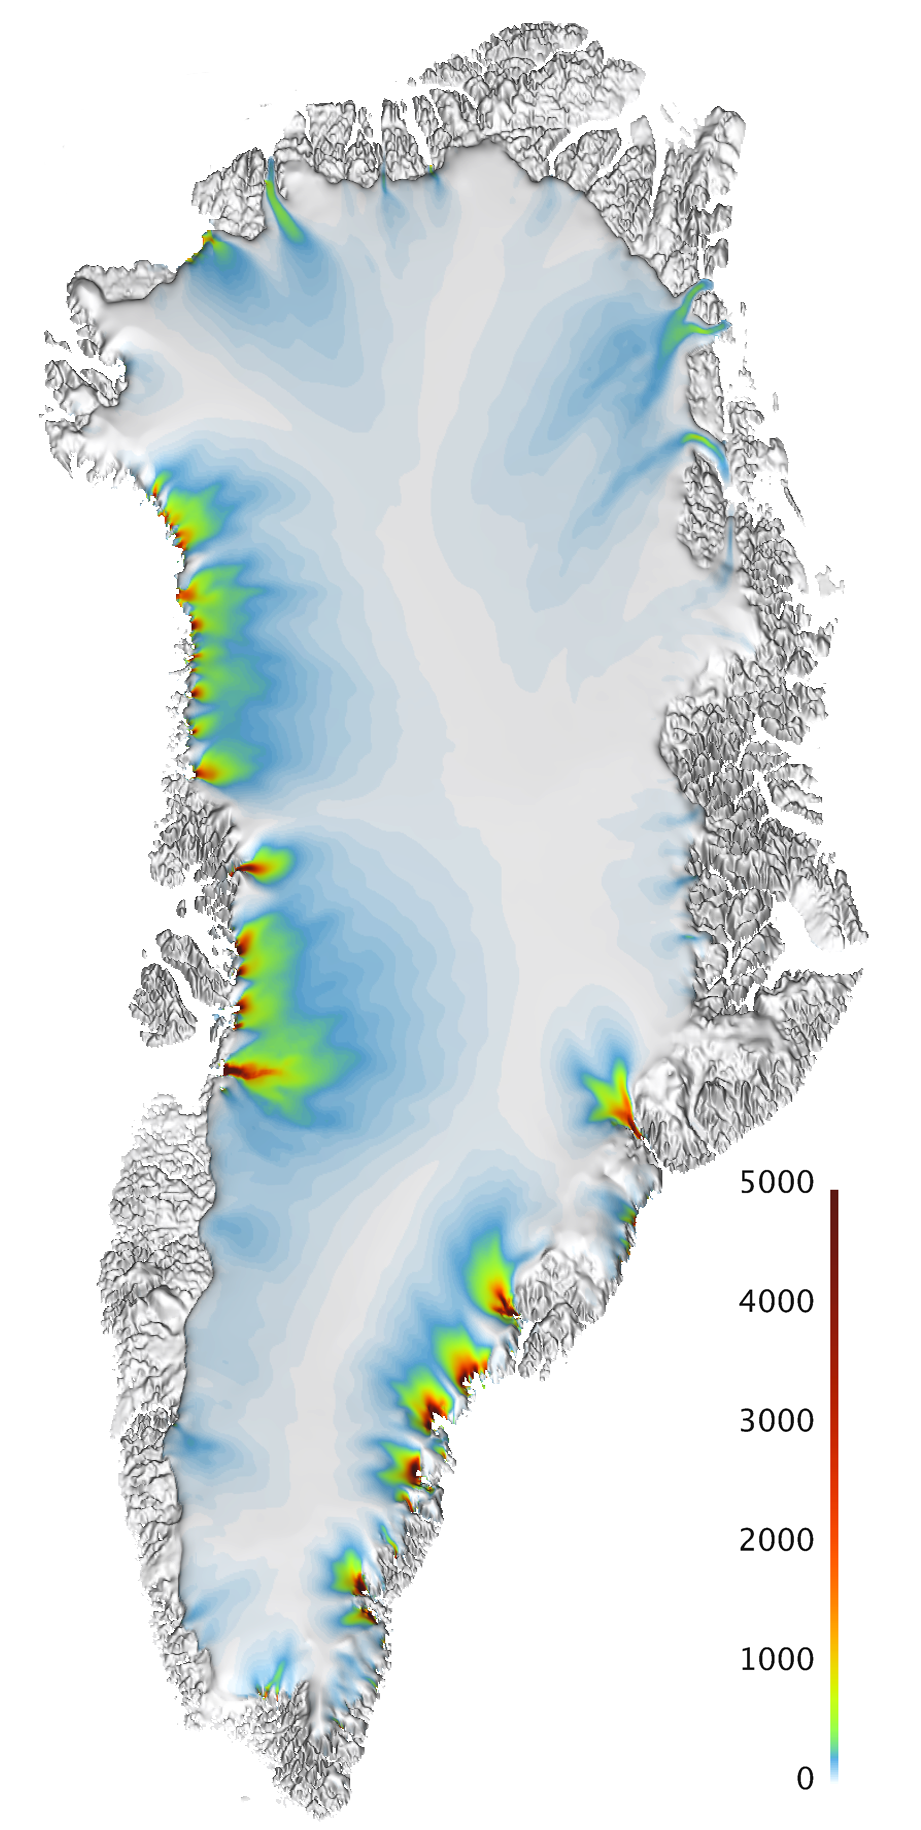
\includegraphics[width=3.in,keepaspectratio=true]{grn-grl-csurf}
    \vfill

    \small Support by email: \texttt{help\@@pism-docs.org}. 

    Manual date \today. Based on PISM \PISMREV.  Needs PETSC release \PETSCREL. \PISMDOWNLOADMSG
  \end{center}
\end{titlepage}

\phantom{bob}
\vspace{1.0in}
\begin{quote}
\textsl{Copyright (C) 2004--2010 Ed Bueler and Constantine Khroulev and Andy Aschwanden and Jed Brown and Nathan Shemonski}
\medskip

\noindent \textsl{This file is part of PISM.}
\medskip

\noindent \textsl{PISM is free software; you can redistribute it and/or modify it under the terms of the GNU General Public License as published by the Free Software Foundation; either version 2 of the License, or (at your option) any later version.  PISM is distributed in the hope that it will be useful, but WITHOUT ANY WARRANTY; without even the implied warranty of MERCHANTABILITY or FITNESS FOR A PARTICULAR PURPOSE.  See the GNU General Public License for more details.  You should have received a copy of the GNU General Public License\index{GPL (\emph{GNU Public License})} along with PISM; see \emph{\texttt{COPYING}}.  If not, write to the Free Software Foundation, Inc., 51 Franklin St, Fifth Floor, Boston, MA  02110-1301 USA}
\end{quote}
\vspace{0.6in}
\normalspacing


\centerline{\textsc{Acknowledgements}}
\bigskip

\small
The NASA Modeling, Analysis, and Prediction program\index{NASA!Modeling, Analysis, and Prediction Program} (grant \# NNX09AJ38G) supports the development of PISM from 2009 to 2013.  We thank them!  Development from 2002 to 2008 was supported by the NASA Cryospheric Sciences Program\index{NASA!Cryospheric Sciences Program}.

The Snow, Ice, and Permafrost (SIP) group\index{Geophysical Institute!Snow, Ice, and Permafrost group} at the Geophysical Institute at UAF is now the home for PISM developers.  Find us in Elvey 410D, in a corner office facing the wilds of Alaska.

The Arctic Region Supercomputing Center\index{Arctic Region Supercomputing Center (ARSC)} has provided significant computational resources and technical help in the development of PISM.

Our research into ice sheet modeling was strongly influenced and constantly motivated by Craig Lingle\index{Lingle, Craig}.  Dave Covey, Don Bahls, and Greg Newby have supported our computers, tools, and computations.  Martin Truffer, Regine Hock, Dani DellaGiustina and others in the SIP group provide the real-glaciology context for PISM at UAF.  Bob Bindshadler, Jesse Johnson, and others in the SeaRISE group have pushed and assisted PISM development in many ways.  Thanks to Tolly Adalgeirsdottir, Torsten Albrecht, Nick Golledge, Marianne Hasselhoff, Tore Hattermann, Anders Levermann, Art Mahoney, Maria Martin, Kent Overstreet, Ben Sperisen, Ward van Pelt, Ricarda Winkelmann, Ryan Woodard, Florian Ziemen and other PISM users/developers for helpful comments and questions on PISM and this \emph{Manual}.
\normalsize

\newpage
\setcounter{tocdepth}{3}
\small
\tableofcontents
\normalsize

\newpage


\section{Introduction}\label{sect:intro}

Welcome!  All information about PISM is online at
\begin{center}
  \href{http://www.pism-docs.org}{\t{www.pism-docs.org}}
\end{center}

This \emph{User's Manual} describes how to run PISM using certain publicly-available data for the Greenland ice sheet and the Ross ice shelf.  It illustrates how PISM's numerical approximations are verified.  It documents all the PISM options.  But it does not explain PISM internals, nor is it a guide for extending the functionality of PISM.

See the \emph{Installation Manual} for how to download\index{PISM!download source code} the PISM source code and install it\index{PISM!install}, along with needed libraries.  It is online at
   \begin{center}
     \href{http://www.pism-docs.org/dev/pdfs/installation-dev.pdf}{\t{www.pism-docs.org/dev/pdfs/installation-dev.pdf}}
   \end{center}

Users who want to understand how PISM works, extend PISM, and/or generally advance the science of ice sheets will need to go beyond what is described here.  For such users there is a \emph{C++ Class Browser}\index{PISM!\emph{C++ Class Browser (HTML)}}.  It gives a complete view of the class/object structure of the PISM source code.  It is the best tool for the job of modifying and supplementing PISM by writing derived classes.  It is online at
   \begin{center}
     \href{http://www.pism-docs.org/dev/doxy/html/index.html}{\t{www.pism-docs.org/dev/doxy/html/index.html}}
   \end{center}

\vspace{.5in}
  
\begin{center}
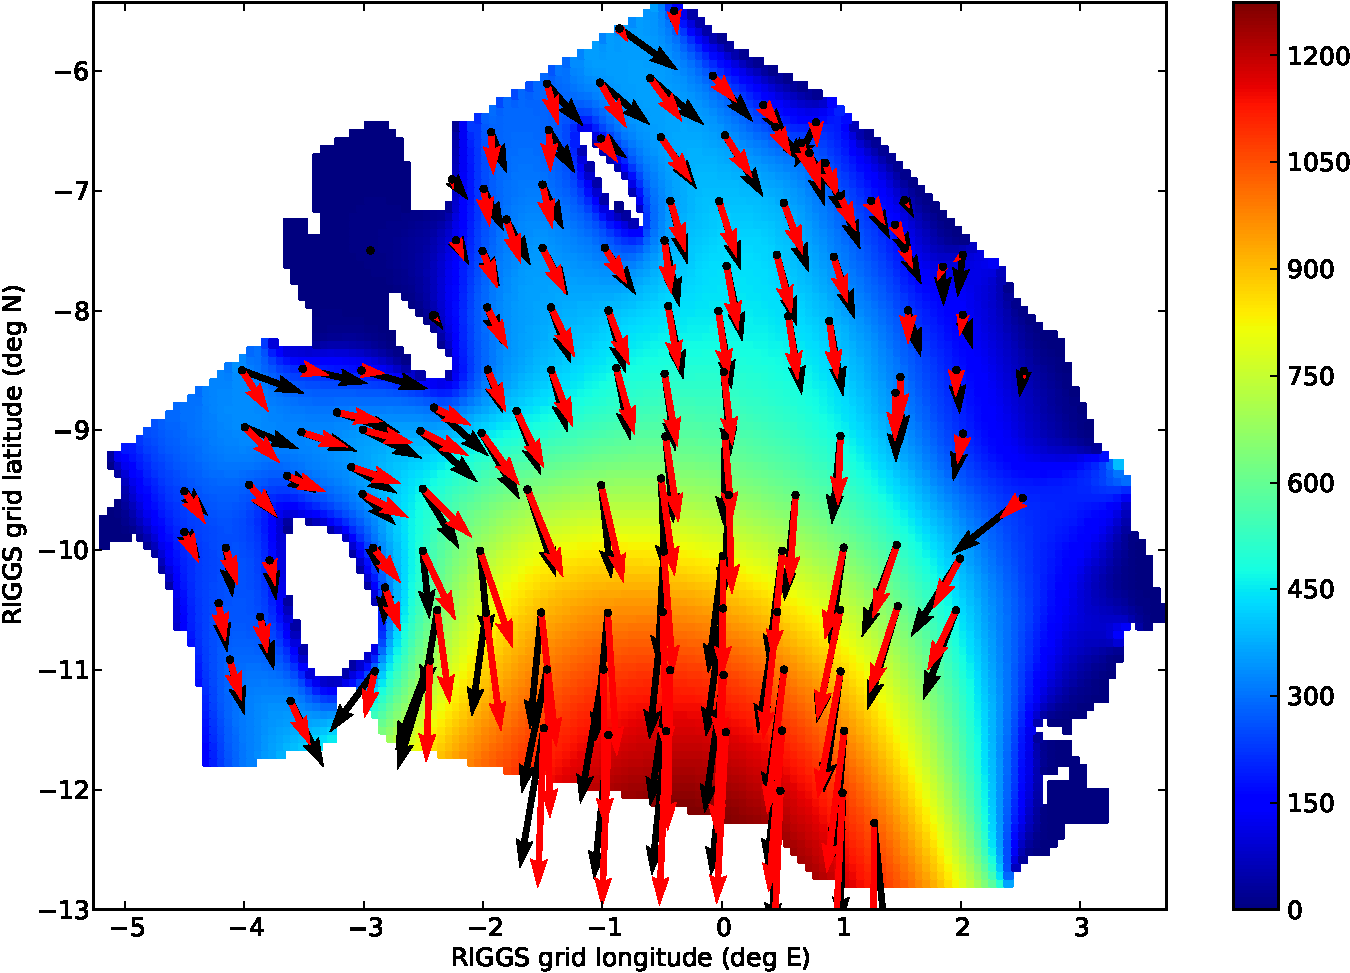
\includegraphics[width=3in,keepaspectratio=true]{rossquiver}
\end{center}

\vspace{.5in}
\large
\begin{center}
\framebox{\parbox{5.0in}{ \emph{WARNING}:\index{PISM!warning}  PISM is an ongoing project.  Ice sheet modeling is complicated and is generally not mature.  Please don't trust the results of PISM or any other ice sheet model without a fair amount of exploration.  Also, please don't expect all your questions to be answered here.  Write to us with questions at \href{mailto:help@pism-docs.org}{\texttt{help@pism-docs.org}}.} }
\normalsize
\end{center}
\normalsize


\clearpage\newpage

\section{Getting started}\label{sec:start}\index{PISM!getting started}

\subsection{On installing PISM}

To install PISM, see the \,\emph{Getting PISM}\, tab at \href{http://www.pism-docs.org}{\texttt{www.pism-docs.org}}.  Or use the PISM Installation Manual (PDF).\footnote{At \url{http://www.pism-docs.org/wiki/lib/exe/fetch.php?media=installation.pdf}.}

Once PISM is installed, the executable \texttt{pismr} should be available on your system's ``path''; confirm this with ``\texttt{which pismr}''.  The instructions below assume you are using a \texttt{bash} shell (or one that accepts \texttt{bash} syntax).  They also assume you have the PISM source code in the directory ``\texttt{pism/}''.

\subsection{A Greenland ice sheet example}

We get started with an extended example showing how to generate initial states for prognostic model experiments on the Greenland ice sheet.  Ice sheet and glacier model studies often involve modeling present and past states using actions like the ones demonstrated in this section.  The particular choices made here are motivated by the evaluation of initialization methods in \cite{AschwandenAdalgeirsdottirKhroulev}.

We use data assembled by the \href{http://websrv.cs.umt.edu/isis/index.php/SeaRISE_Assessment}{Sea-level Response to Ice Sheet Evolution (SeaRISE)} group \cite{Bindschadler2013SeaRISE}.  SeaRISE was a community-organized assessment process providing an upper bound on ice sheet contributions to sea level in the next 100--200 years, especially for the IPCC AR5 report in 2013.

This example is a hands-on first look at PISM.  It is not an in-depth tutorial, and some details of what is happening will only be explained later.  The remainder of this manual lists PISM options, discusses nontrivial modeling choices, and explains the ways users may need to preprocess input data.

Some of the PISM output figures in this section were produced using a supercomputer.  Though the basic run here, on a rather coarse $20\,\textrm{km}$ grid, can be done on a typical workstation or laptop, PISM is designed to make high resolution possible by exploiting large-scale parallel processing \cite[among many other examples]{AschwandenAdalgeirsdottirKhroulev,Golledgeetal2012,Golledgeetal2013}.


\subsection{Input data}

The NetCDF data used to initialize SeaRISE runs is freely-available online: 
\medskip

\centerline{\protect{\textbf{\url{http://websrv.cs.umt.edu/isis/index.php/Present_Day_Greenland}}}}
\medskip

\noindent The quickest way to get the file is to do
\begin{verbatim}
$ cd pism/examples/std-greenland
$ ./preprocess.sh
\end{verbatim}
\noindent The script \texttt{preprocess.sh} requires \texttt{wget} and also the NetCDF Operators (``NCO''; \url{http://nco.sourceforge.net/}).  It downloads the version 1.1 of the SeaRISE ``master'' present-day data set, which contains ice thickness and bedrock topography from BEDMAP \cite{BamberLayberryGogenini}, and modeled precipitation rates from RACMO \cite{Ettemaetal2009}, among other fields.

In particular, it creates three new NetCDF files which can be read by PISM.  The spatially-varying fields from the downloaded ``master'' file, with adjusted metadata, go in the PISM-readable file \texttt{pism_Greenland_5km_v1.1.nc}.  The other two new files contain famous time-dependent paleo-climate records from ice core and seabed core records; \texttt{pism_dT.nc} has GRIP \cite{JohnsenetalGRIP} while \texttt{pism_dSL.nc} has SPECMAP \cite{Imbrieetal1984}.

Any of these NetCDF files can be viewed with \texttt{ncview} or other NetCDF visualization tools; see Table \ref{tab:NetCDFview} below.  An application of IDV to the master data set produced Figure \ref{fig:sr-input}, for example.  Use \texttt{ncdump -h} to see the metadata and history of the files.

\begin{figure}[ht]
\centering
\mbox{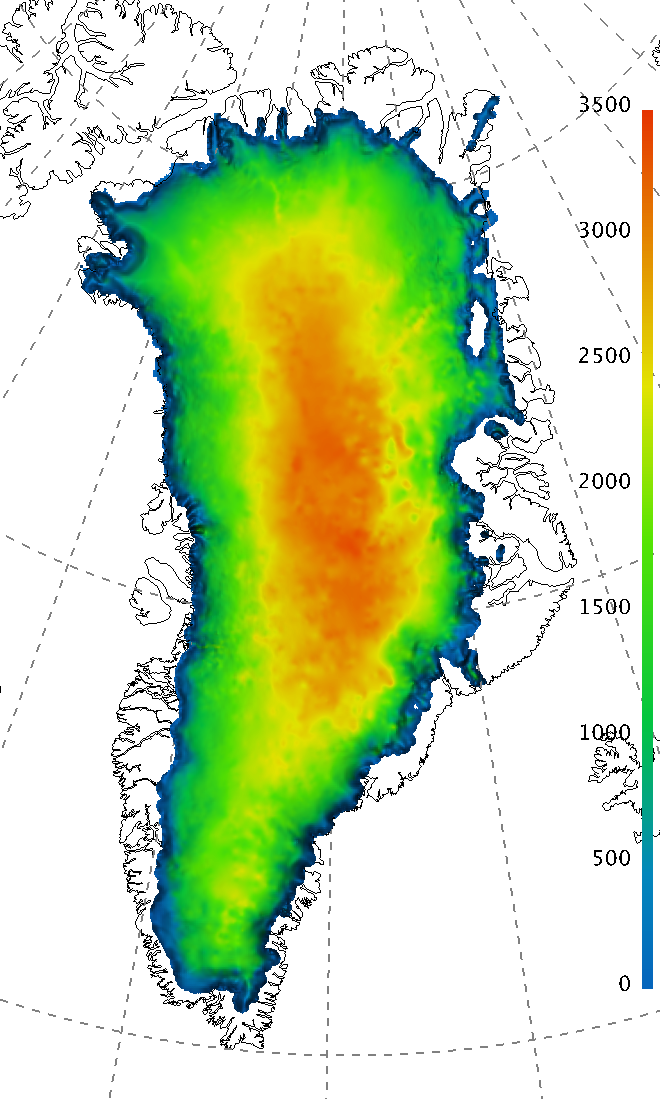
\includegraphics[width=2.0in,keepaspectratio=true]{sr-greenland-thk}
  \qquad
  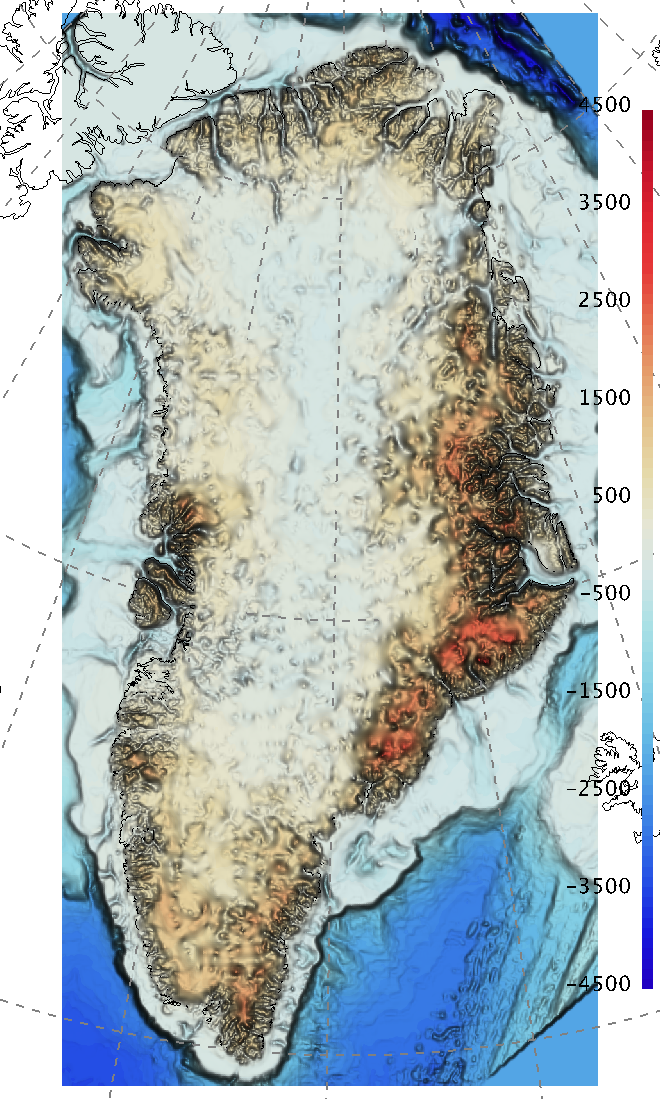
\includegraphics[width=2.0in,keepaspectratio=true]{sr-greenland-topg}
  \qquad
  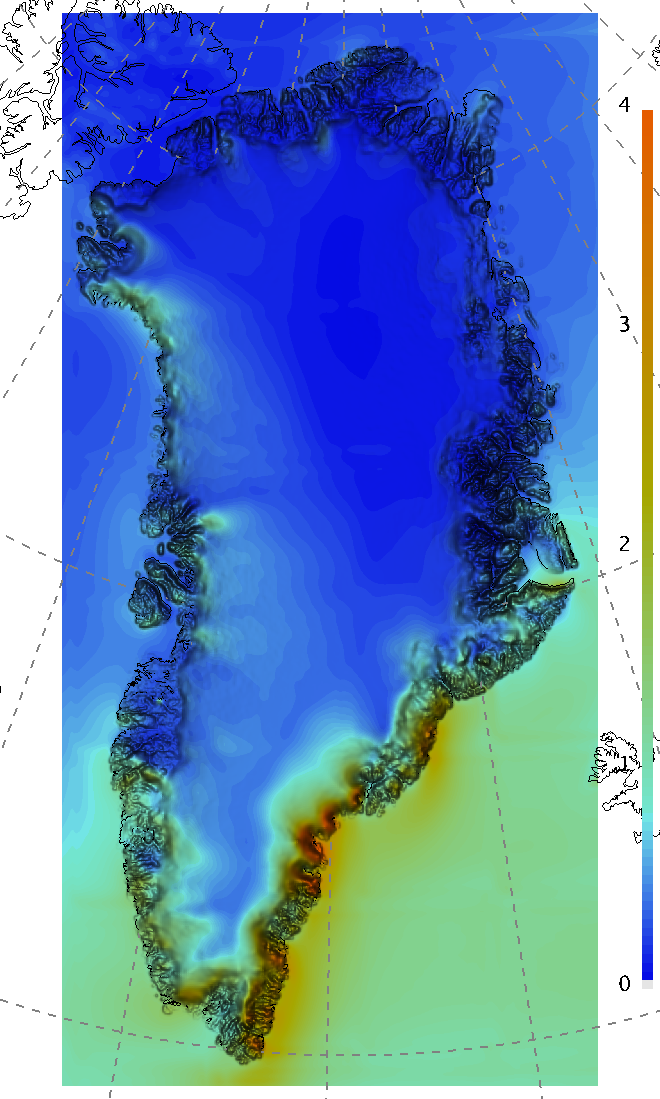
\includegraphics[width=2.0in,keepaspectratio=true]{sr-greenland-prcp}}
\caption{The input present-day ice thickness (left; m), bedrock elevation (center; m), and present-day precipitation (right; m $\text{a}^{-1}$ ice equivalent) for SeaRISE-Greenland.  These are fields \texttt{thk}, \texttt{topg}, and \texttt{precipitation}, respectively, in file \texttt{pism_Greenland_5km_v1.1.nc} produced by running \texttt{preprocess.sh}.}
\label{fig:sr-input}
\end{figure}


\subsection{First run}   \label{subsect:runscript}  Like many Unix programs, PISM allows many command-line options.  Because PISM handles a wide variety of ice sheet, shelf, and glacier sub-models and configurations, the list of possible command-line options is long; see sections \ref{sec:boot} through \ref{sec:practical-usage} of this manual.  Therefore, in practice, one often builds scripts to run PISM with the correct options.

Our script is called ``\texttt{spinup.sh}''.  Initializing ice sheets can be done by computing approximate steady states with constant boundary data, or, in some cases, by integrating paleo-climatic and long-time-scale information to build a model for the present state of the ice sheet.  Both of these possibilities are illustrated in the \texttt{spinup.sh} script.  The spin-up stage may even require the most processor-hours, compared to a follow-on ``experiment'' or ``forecast'' stages.

We are ready to run PISM.  To see what can be done with the script, read the usage message it produces:
\begin{verbatim}
$ ./spinup.sh
\end{verbatim}

The simplest spin-up approach is to use a ``constant-climate'' model.  We take this approach first.  To see a more detailed view of the run we will do first, try:
\begin{verbatim}
$ PISM_DO=echo ./spinup.sh 4 const 10000 20 sia g20km_10ka.nc
\end{verbatim}
Setting the environment variable \texttt{PISM_DO} in this way tells \texttt{spinup.sh} just to print out the commands it is about to run, not do them.  The ``proposed'' run looks like this:
\small
\begin{verbatim}
mpiexec -n 4 pismr -boot_file pism_Greenland_5km_v1.1.nc -Mx 76 -My 141 \
  -Mz 101 -Mbz 11 -z_spacing equal -Lz 4000 -Lbz 2000 -skip -skip_max 10 \
  -ys -10000 -ye 0 -surface given -surface_given_file pism_Greenland_5km_v1.1.nc \
  -ocean_kill pism_Greenland_5km_v1.1.nc -sia_e 3.0 \
  -ts_file ts_g20km_10ka.nc -ts_times -10000:yearly:0 \
  -extra_file ex_g20km_10ka.nc -extra_times -10000:100:0 \
  -extra_vars diffusivity,temppabase,tempicethk_basal,bmelt,tillwat,csurf,mask,thk,topg,usurf \
  -o g20km_10ka.nc
\end{verbatim}
\normalsize
Let's briefly deconstruct this run.

At the front is ``\texttt{mpiexec -n 4 pismr}''.  This means that the PISM executable \texttt{pismr} is run in parallel on four processes (e.g.~cores).  Though this example assumes you have a workstation or laptop with at least 4 cores, it will work with 1 to 100 processors, with reasonably good scaling in speed.  (Scaling can be good with far more processors if we run at higher spatial resolution.)  The executable name ``\texttt{pismr}'' stands for the standard ``run'' mode of PISM, in contrast to other, specialized modes described later (e.g.~in sections \ref{sec:verif} and \ref{sec:simp}).

Next, the proposed run uses option \texttt{-boot_file} to start the run by ``bootstrapping,'' a term describes the creation, by heuristics and highly-simplified models, of the complete initial conditions required for a deterministic, time-dependent ice dynamics model.  Then the options describe a $76\times 141$ point grid in the horizontal, which gives 20 km grid spacing in both directions.  Then there are choices about the vertical extent and resolution of the computational grid; more on those later.  After that we see a description of the time-axis, with a start and end time given: ``\texttt{-ys -10000 -ye 0}''.

Then we get the instructions that tell PISM to read the upper surface boundary conditions (i.e.~climate) from a file: ``\texttt{-surface given -surface_given_file pism_Greenland_5km_v1.1.nc}''.  For more on these choices, see subsection \ref{sec:climate-inputs}, and also the PDF PISM Climate Forcing Manual.

Following that there are longish options describing the fields we want as output, including scalar time series (``\texttt{-ts_file ts_g20km_10ka.nc -ts_times -10000:yearly:0}''; see section \ref{sec:practical-usage}), time- and space-dependent fields (``\texttt{-extra_file ...}''; again see section \ref{sec:practical-usage}), and finally the named output file (``\texttt{-o g20km_10ka.nc}'').

Now let's actually get the run going:
\begin{verbatim}
$ ./spinup.sh 4 const 10000 20 sia g20km_10ka.nc &> out.g20km_10ka &
\end{verbatim}
\noindent The terminating ``\verb|&|'' asks unix to run the command in the background, so we can keep working in the current shell.  Because we have re-directed the text output, PISM will show what it is doing in the text file \texttt{out.g20km_10ka}.  Using \texttt{less} is a good way to watch such a growing text-output file.


\subsection{Watching the first run}  \label{subsect:watchrun}  The next paragraphs describe what happens and what files are produced by the run which is underway.  The modeling choices represented here are reasonable, but they are not the only way to do it.  The user is encouraged to experiment; that is the point of a model!

As soon as the run starts it creates time-dependent NetCDF files \texttt{ts_g20km_10ka.nc} and \texttt{ex_g20km_10ka.nc}.  Actually the latter file spatially-dependent file is created after the first 100 years of model run, but that is a few seconds in this case.  In fact, the command \texttt{-extra_file ex_g20km_10ka.nc -extra_times -10000:100:0} will add a spatially-dependent ``frame'' at model times -9900, -9800, \dots, 0.  One way to get a snapshot of how many frames this file contains at any time is to do
\begin{verbatim}
$ ncdump -h ex_g20km_10ka.nc |grep "time ="
\end{verbatim}
but a more interactive way is to look at the output graphically with
\begin{verbatim}
$ ncview ex_g20km_10ka.nc
\end{verbatim}
In any case, we see that \texttt{ex_g20km_10ka.nc} contains ``movies'' of the fields chosen by the option \texttt{-extra_vars diffusivity,...,thk,topg,usurf}.  A frame of the ice thickness \texttt{thk} is shown in Figure \ref{fig:growing} (left).

The time-series file \texttt{ts_g20km_10ka.nc} is also growing.  It contains spatially-averaged ``scalar'' diagnostics like the total ice volume or the ice-sheet-wide maximum velocity (variable \texttt{ivol} and \texttt{max_hor_vel}, respectively).  It can be viewed
\begin{verbatim}
$ ncview ts_g20km_10ka.nc
\end{verbatim}
Generally PISM ``buffers'' its time series, so the file may only be updated when the buffer is full (see section \ref{sec:saving-time-series}), but, as the buffer is also cleared everytime a frame is written to an \texttt{-extra_file}, in this case the file \texttt{ts_g20km_10ka.nc} is updated frequently.  The growing time series for \texttt{ivol} is shown in Figure \ref{fig:growing} (right).  After such inspections of the diagnostic files \texttt{ex_g20km_10ka.nc} and \texttt{ts_g20km_10ka.nc}, the reader will agree that PISM can produce quite a bit of information about a run, but in a user-controllable manner.

\begin{figure}[ht]
\centering
\mbox{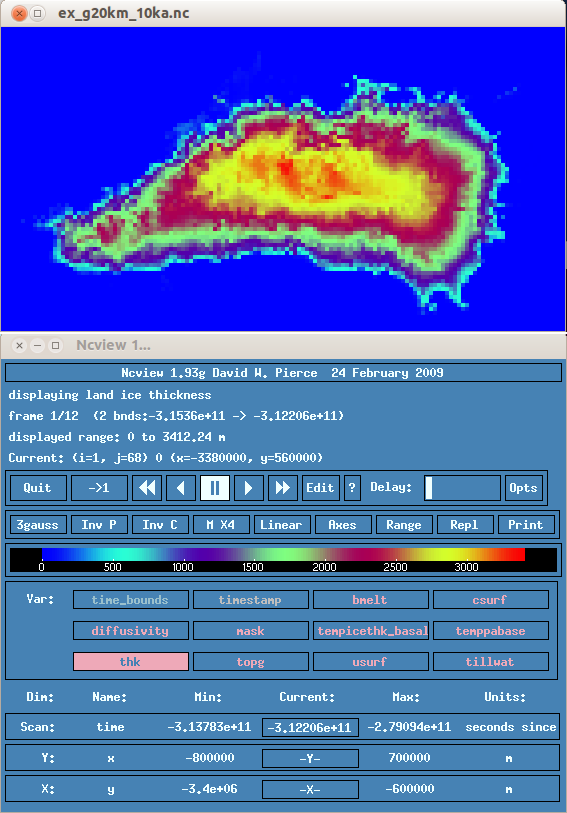
\includegraphics[height=5.0in,keepaspectratio=true]{ex-growing-thk-g20km}
  \qquad 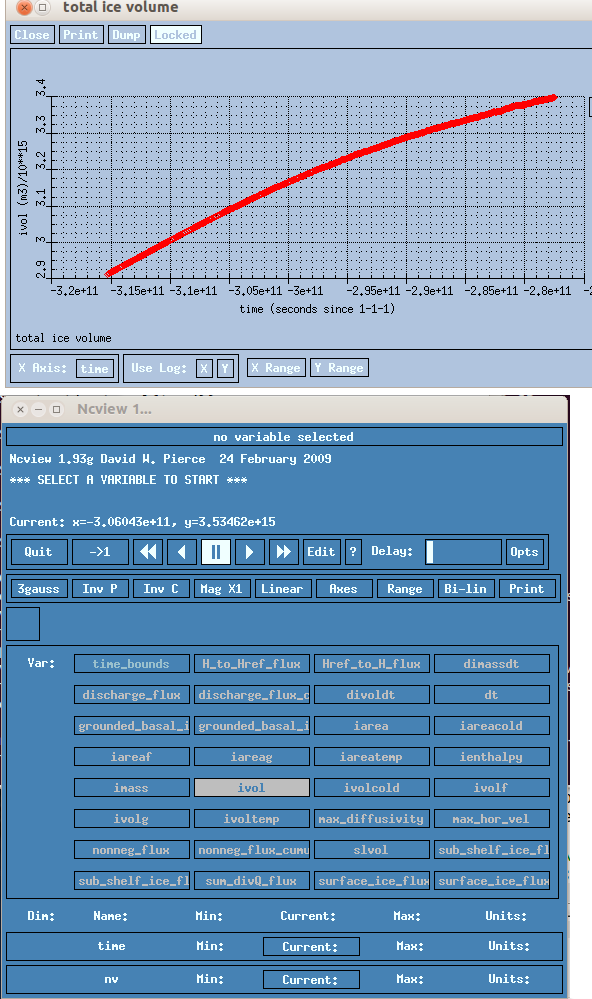
\includegraphics[height=5.0in,keepaspectratio=true]{ts-growing-ivol-g20km}}
\caption{Two views produced by \texttt{ncview} during a PISM model run for the Greenland ice sheet.  Left: Field \texttt{thk}, the ice sheet thickness, a space-dependent frame from file \texttt{ex_g20km_10ka.nc}.  Right: Time-series \texttt{ivol}, the total ice sheet volume, from file \texttt{ts_g20km_10ka.nc}. }
\label{fig:growing}
\end{figure}

At the end of the run the output file \texttt{g20km_10ka.nc} is generated.  To see a report on computational  performance, we do:
\begin{verbatim}
$ ncdump -h g20km_10ka.nc |grep history
    :history = "user@machine 2013-11-23 15:57:22 AKST: PISM done.  Performance stats:
0.3435 wall clock hours, 1.3738 proc.-hours, 7274.0065 model years per proc.-hour,
PETSc MFlops = 0.03.\n",
\end{verbatim}
The whole first run took about 21 minutes (0.3435 wall clock hours) on a 2012-era 4-core laptop.

The intention of this run was to generate a minimal model of the Greenland ice sheet in approximate steady-state with a steady (constant-in-time) climate.  Figure \ref{fig:firstoutput} shows some fields from \texttt{g20km_10ka.nc}.  In the next subsection  we will start discussing their ``quality'' as model results.

\begin{figure}[ht]
\centering
\mbox{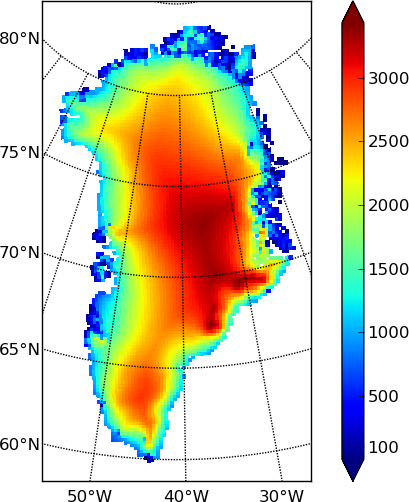
\includegraphics[height=2.75in,keepaspectratio=true]{g20km-10ka-usurf} 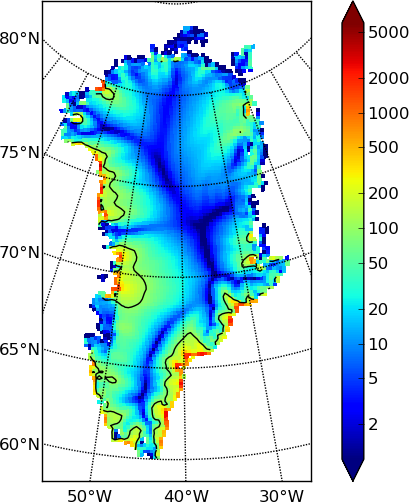
\includegraphics[height=2.75in,keepaspectratio=true]{g20km-10ka-csurf} 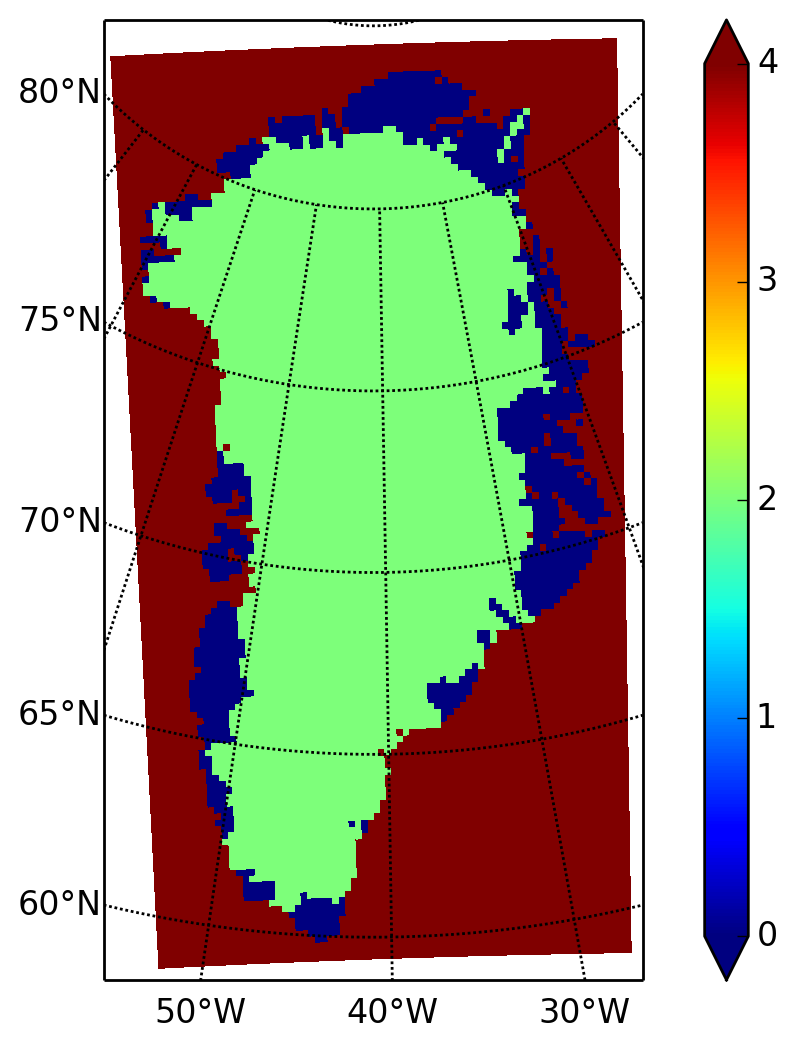
\includegraphics[height=2.75in,keepaspectratio=true]{g20km-10ka-mask}}
\caption{Fields from output file \texttt{g20km_10ka.nc}.  Left: \texttt{usurf}, the ice sheet surface elevation in meters.  Middle: \texttt{csurf}, the surface velocity in meters/year ($=$ m/a), including the 100 m/a contour (solid black).  Right: \texttt{mask}, with 0 = ice-free land, 2 = ice, 4 = ice-free ocean.}
\label{fig:firstoutput}
\end{figure}


\subsection{Second run: a better ice-dynamics model}  \label{subsect:ssarun}  

It is widely-understood that ice sheets slide on their bases, especially when liquid water is present at the base (see \cite{Joughinetal2001,MacAyeal}, among many others).  An important aspect of modeling such sliding is the inclusion of membrane or ``longitudinal'' stresses into the stress balance \cite{BBssasliding}.  The basic stress balance in PISM which uses membrane stresses is the Shallow Shelf Approximation (SSA) \cite{WeisGreveHutter}.  The stress balance used in the previous section was, by contrast, the (thermomechanically-coupled) non-sliding, non-membrane-stress Shallow Ice Approximation (SIA) \cite{BBL,EISMINT00}.  The preferred ice dynamics model within PISM, that allows both sliding balanced by membrane stresses and shear flow as described by the SIA, is the SIA+SSA ``hybrid'' model \cite{BBssasliding,Winkelmannetal2011}.  For more on such theory see section \ref{sec:dynamics} of the current \emph{Manual}.

The practical disadvantage of models of sliding is that a distinctly-uncertain parameter space must be introduced.  This especially involves parameters controlling the amount and pressure of subglacial water (see \cite{AschwandenAdalgeirsdottirKhroulev,Clarke05,Tulaczyketal2000,vanPeltOerlemans2012} among other references).  In this regard, PISM uses the concept of a saturated and pressurized subglacial till with a modeled distribution of yield stress  \cite{BBssasliding,SchoofStream}.  The yield stress arises from the PISM model of the production of subglacial water, which is itself computed through the conservation of energy model \cite{AschwandenBuelerKhroulevBlatter}.

We use such models in the rest of this Getting Started section.  We will show some steps which analyze the difference between observed and modeled surface velocity of the Greenland ice sheet.  While the \texttt{spinup.sh} script has default sliding parameters, for demonstration purposes we change one parameter; we replace the default power $q=0.25$ in the sliding law, an equation which relates both the subglacial sliding velocity and the till yield stress to the basal shear stress which appears in the SSA stress balance, by a less ``plastic'' choice $q=0.5$.  (See subsection \ref{subsect:basestrength} for more on this important parameter, and other related parameters.)

To see the run we propose, do
\begin{verbatim}
$ PISM_DO=echo PARAM_PPQ=0.5 ./spinup.sh 4 const 10000 20 hybrid g20km_10ka_hy.nc
\end{verbatim}
Now remove the setting of \texttt{PISM_DO} and redirect the text output into a file, and start the run:
\begin{verbatim}
$ PARAM_PPQ=0.5 ./spinup.sh 4 const 10000 20 hybrid g20km_10ka_hy.nc &> out.g20km_10ka_hy &
\end{verbatim}

Surprisingly perhaps,\footnote{The reason this hybrid run is quicker is fairly deep.  Though the computation of the SSA stress balance is substantially more expensive than the SIA in a per-step sense---and in fact the hybrid model is doing both the SIA and SSA computation at each step!---the SSA stress balance in combination with the mass continuity equation causes the maximum diffusivity in the ice sheet to be substantially lower during the run.  Because the maximum diffusivity controls the time-step in the PISM adaptive time-stepping scheme \cite{BBL}, the number of time steps is so much reduced that the run takes half the time.  (To see this contrast do ``\texttt{ncview ts_g20km_10ka*nc} and view variables \texttt{max_diffusivity} and \texttt{dt}.) } this finishes in half the time of the computation in the previous section, about 10 minutes (0.1649 wall clock hours) on a 2012-era 4-core laptop:
\begin{verbatim}
$ ncdump -h g20km_10ka_hy.nc |grep history
    :history = "user@machine 2013-11-23 17:36:55 AKST: PISM done.  Performance stats:
0.1649 wall clock hours, 0.6598 proc.-hours, 15146.2867 model years per proc.-hour,
PETSc MFlops = 264118.55.\n",
\end{verbatim}
Note that the number reported as ``\texttt{PETSc MFlops}'' is many orders of magnitude larger because calls to the PETSc library are used when solving the non-local SSA stress balance.

The results of this run are shown in Figure \ref{fig:secondoutputcoarse}.  We show the basal sliding speed field \texttt{cbase} in this Figure.  (Replacing \texttt{mask} in Figure \ref{fig:firstoutput}; the reader can check that \texttt{cbase}=0 in the SIA-only result \texttt{g20km_10ka.nc}.)

\begin{figure}[ht]
\centering
\mbox{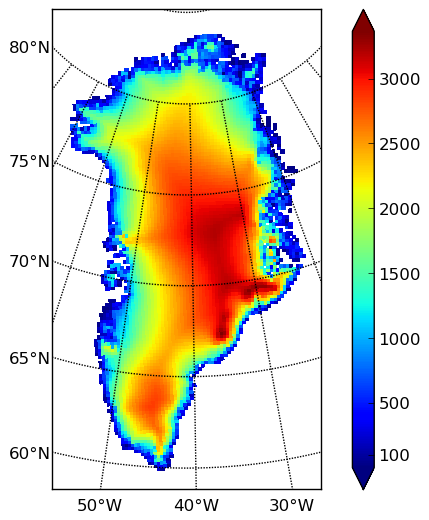
\includegraphics[height=2.75in,keepaspectratio=true]{g20km-10ka-hy-usurf} 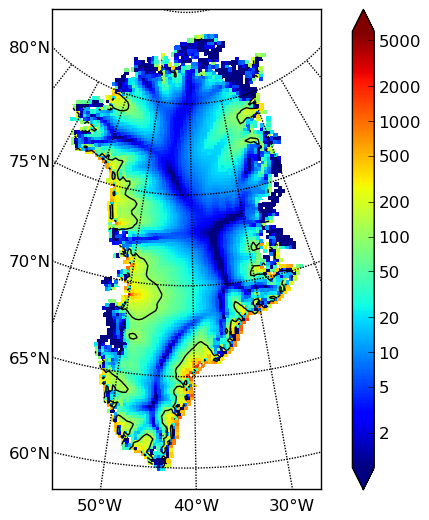
\includegraphics[height=2.75in,keepaspectratio=true]{g20km-10ka-hy-csurf} 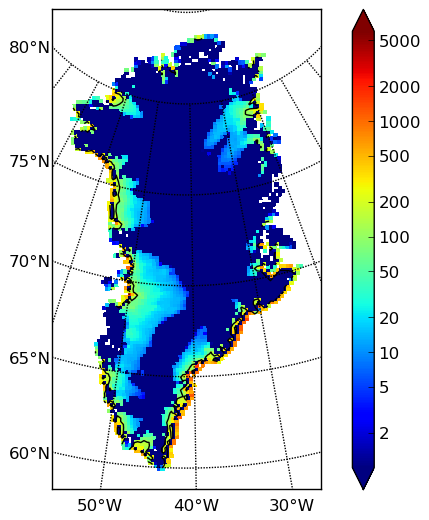
\includegraphics[height=2.75in,keepaspectratio=true]{g20km-10ka-hy-cbase}}
\caption{Fields from output file \texttt{g20km_10ka_hy.nc}.  Left: \texttt{usurf}, the ice sheet surface elevation in meters.  Middle: \texttt{csurf}, the surface velocity in m/a, including the 100 m/a contour (solid black).  Right: \texttt{cbase}, shown the same way as \texttt{csurf}.}
\label{fig:secondoutputcoarse}
\end{figure}

The basal sliding velocity, though critical to the response of the ice to changes in climate, is essentially unobservable.  On the other hand, at the present state of technology the surface velocity of an ice sheet is an observable.\footnote{This is because of relatively-recent advances in radar and image technology and processing \cite{Joughin2002}.}  So, how good is our model result for \texttt{csurf}?  The left-hand two parts of Figure \ref{fig:csurfvsobserved} compare the \texttt{surfvelmag} field in the downloaded SeaRISE-Greenland data file \texttt{Greenland_5km_v1.1.nc} with the just-computed PISM result.  The reader might agree with these broad qualitative judgements:
\begin{itemize}
\item the model results and the observed surface velocity look similar, but
\item in the model, southern Greenland has fast-flowing ice at the margin, while the observations show much more localized flow, and
\item the observed Northeast Greenland ice stream is much more distinct than shown in the model.
\end{itemize}
Of course, this is just one model of many ``in'' PISM.  We are free to find and adjust important parameters.  The first we address is one of the most important: grid resolution.

First, though, in considering these PISM results compared to some recent observed-vs-model comparisons of this type (e.g.~Figure 1 in \cite{Priceetal2011} and Figure 8 in \cite{Larouretal2012}), note that only ice-sheet-wide parameters and models were used.  Each location in the ice sheet was modeled by the same physics.  Specifically there was no attempt to tune a large number of subglacial parameters to values which would yield close match to observations of the surface velocity.  Such tuning techniques are called ``inversions''; see \cite{vanPeltetal2013} (basal topography) and \cite{Habermannetal2013} (basal shear stress) for PISM-based inversion methods and analysis.

As noted, we change one key parameter first, the grid resolution.  If you can let it run overnight on a laptop,\footnote{Or change ``\texttt{4}'' in the call to \texttt{spinup.sh} to a substantially larger number, on a supercomputer.} do
\begin{verbatim}
$ PARAM_PPQ=0.5 ./spinup.sh 4 const 10000 10 hybrid g10km_10ka_hy.nc &> out.g10km_10ka_hy &
\end{verbatim}
This run takes about four hours on a 2012-era 4 core laptop.  We see some fields from the result in Figure \ref{fig:secondoutputfiner}.

\begin{figure}[ht]
\centering
\mbox{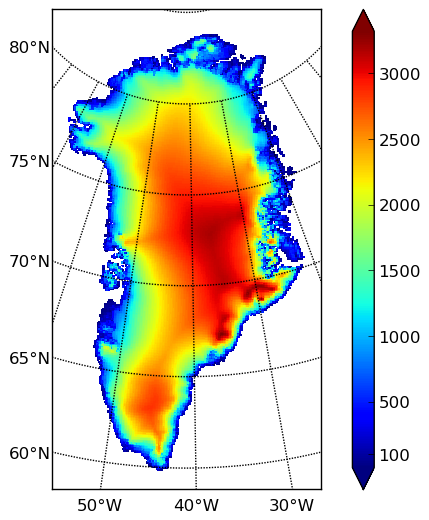
\includegraphics[height=2.75in,keepaspectratio=true]{g10km-10ka-hy-usurf} 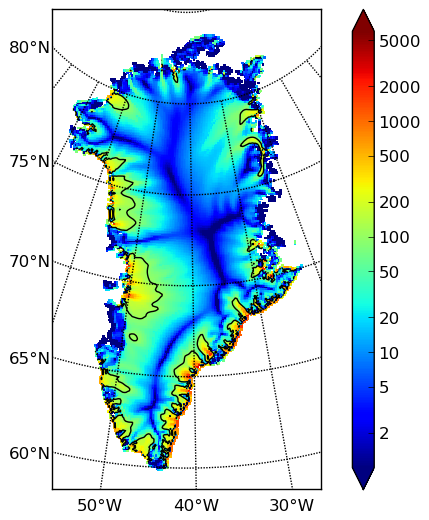
\includegraphics[height=2.75in,keepaspectratio=true]{g10km-10ka-hy-csurf} 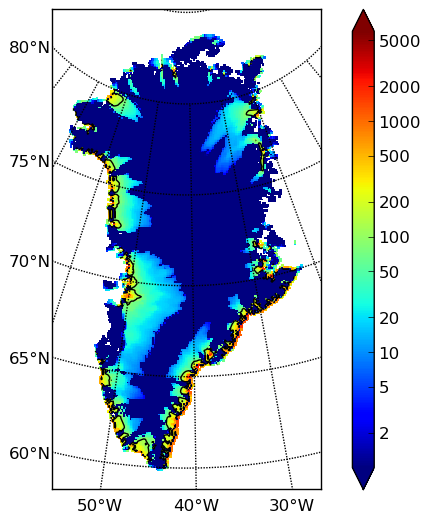
\includegraphics[height=2.75in,keepaspectratio=true]{g10km-10ka-hy-cbase}}
\caption{Fields from output file \texttt{g10km_10ka_hy.nc}.  Left: \texttt{usurf} in meters.  Middle: \texttt{csurf} in m/a.  Right: \texttt{cbase} in m/a.}
\label{fig:secondoutputfiner}
\end{figure}

Figure \ref{fig:csurfvsobserved} compares observed velocity to the model results from 20 km and 10 km grids.  Model results differ, of course, even when the only change is the resolution.  Importantly for ice sheet modeling, higher resolution model runs ``pick up'' higher resolution bed elevation and climate data.

\begin{figure}[ht]
\centering
\mbox{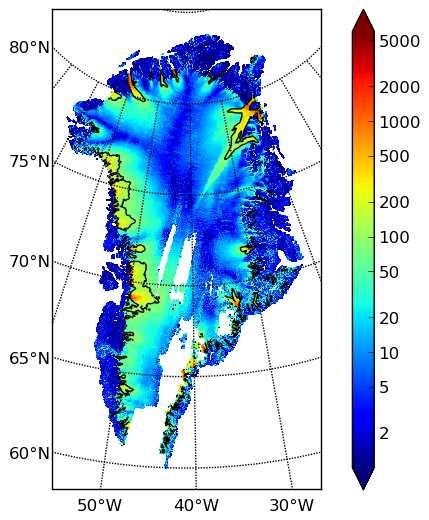
\includegraphics[height=2.75in,keepaspectratio=true]{Greenland-5km-v1p1-surfvelmag} 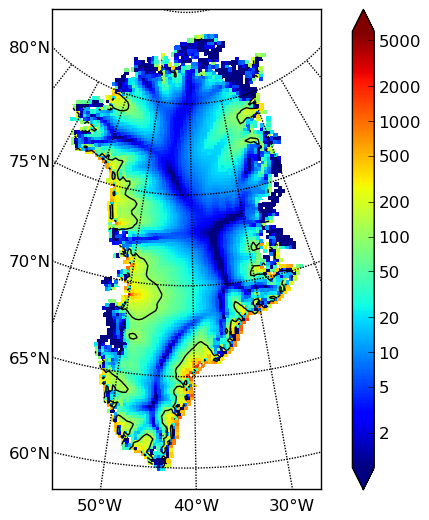
\includegraphics[height=2.75in,keepaspectratio=true]{g20km-10ka-hy-csurf} 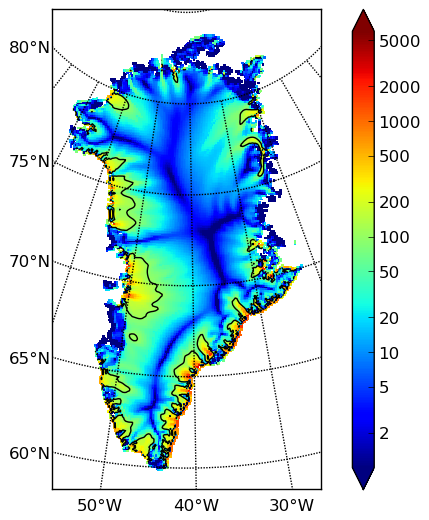
\includegraphics[height=2.75in,keepaspectratio=true]{g10km-10ka-hy-csurf}}
\caption{Comparing modeled surface speed to observations.  All are in m/a with 100 m/a contour solid black.  Left: \texttt{surfvelmag}, the observed values from SeaRISE data file \texttt{Greenland_5km_v1.1.nc}.  Middle: \texttt{csurf} from \texttt{g20km_10ka_hy.nc}.  Right: \texttt{csurf} from \texttt{g10km_10ka_hy.nc}.}
\label{fig:csurfvsobserved}
\end{figure}

As a different kind of comparison, Figure \ref{fig:ivolboth} shows ice volume time series \texttt{ivol} for 20km and 10km runs done here.  We see that this result depends on resolution, in particular because higher resolution grids allow the model to better resolve the flux through topographically-controlled outlet glaciers (compare \cite{Pfefferetal2008}).  However, because the total ice sheet volume is a highly-average quantity, the \texttt{ivol} difference from 20km and 10km resolution runs is only about one part in 60 (about 1.5\%) at the final time.  By contrast, as is seen in the near-margin ice in various locations shown in Figure \ref{fig:csurfvsobserved}, the ice velocity at a particular location may change by 100\% when the resolution changes from 20km to 10km.  Roughly speaking, the reader should only trust model results which are demonstrated to be robust across a range of model parameters, and, in particular, which are shown to be relatively-stable among relatively-high resolution results for a particular case.  Using a supercomputer is, in fact, often justified merely to confirm that lower-resolution runs were already ``getting'' a given feature in model results.

\begin{figure}[ht]
\centering
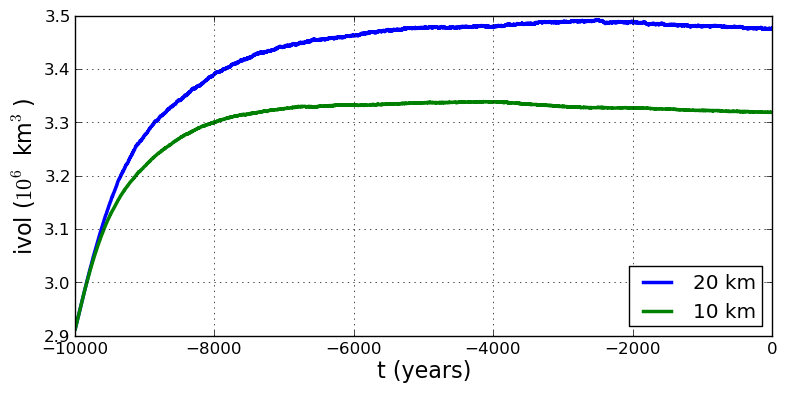
\includegraphics[width=4.0in,keepaspectratio=true]{ivol-both-g20km-g10km}
\caption{Time series of modeled ice sheet volume on 20km and 10km grids.  The present-day ice sheet has volume approximately $2.91\times 10^6\,\text{km}^3$, the initial value in both runs.}
\label{fig:ivolboth}
\end{figure}


\subsection{Third run: paleo-climate model spin-up}  \label{subsect:paleorun}  


\begin{figure}[ht]
\centering
%  temppabase from last time in ex_g10km_steady.nc and driving stress taud from g10km_SIA.nc
%\mbox{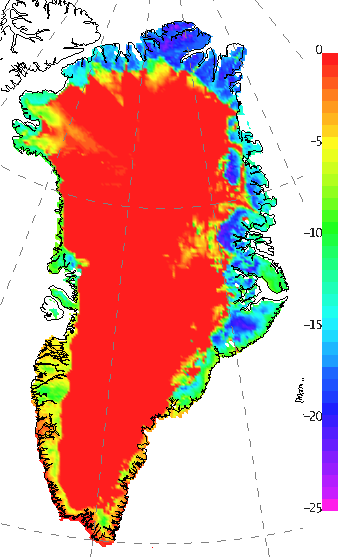
\includegraphics[width=2.0in,keepaspectratio=true]{temppabase}
%  \qquad 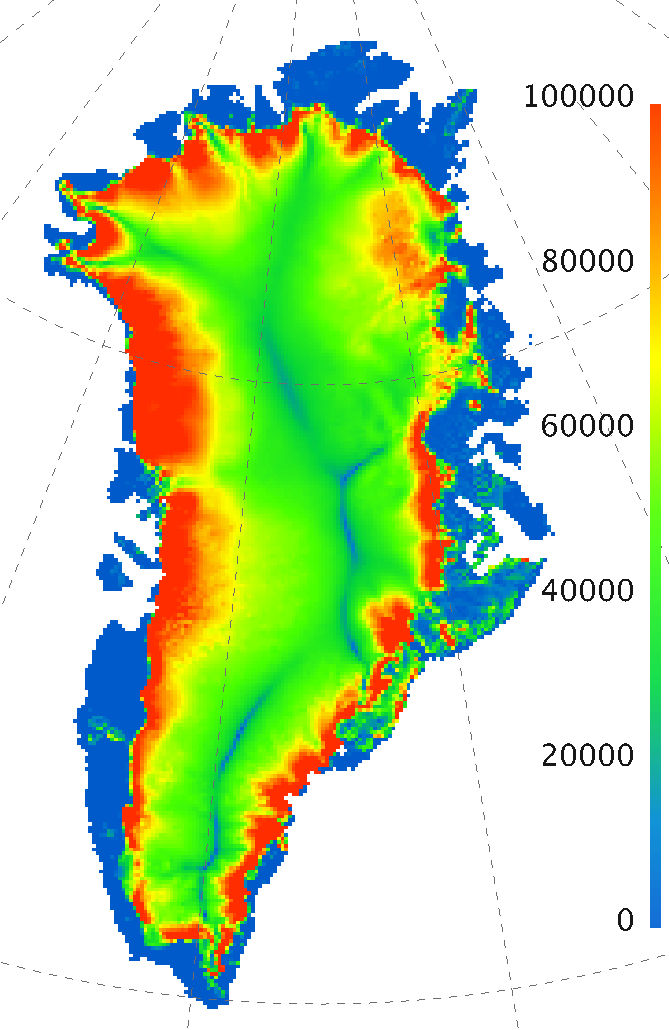
\includegraphics[width=2.1in,keepaspectratio=true]{taud}}
\caption{FIXME: Part of the model state at the beginning of paleo-climate-modeling ice sheet spin-up, in file \texttt{g20km_steady.nc} from running \texttt{spinup.sh}.  Left: pressure-adjusted basal temperature ($\phantom{|}^\circ$C; field \texttt{temp_pa}).  Right: driving stress magnitude $\rho g H |\grad h|$ (Pa; field \texttt{taud_mag}).}
\label{fig:sr-spinstart}
\end{figure}


\begin{figure}[ht]
\centering
%  thk, cbase, csurf from g10km_0.nc
%\mbox{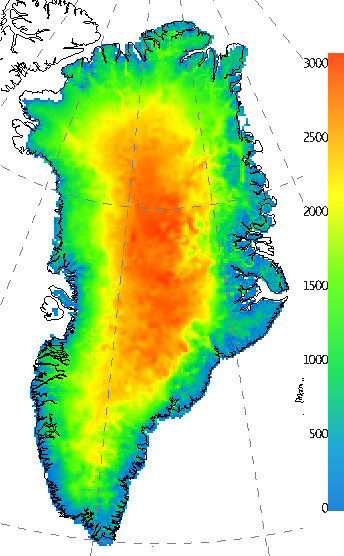
\includegraphics[width=2.in,keepaspectratio=true]{thk}
%  \qquad 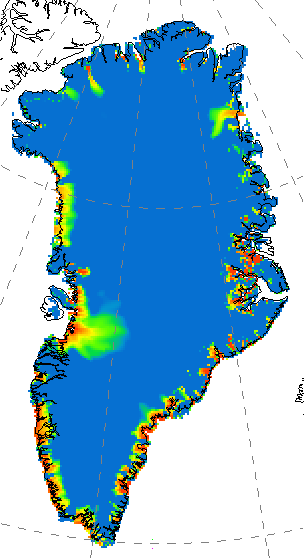
\includegraphics[width=2.in,keepaspectratio=true]{cbase}
%  \qquad 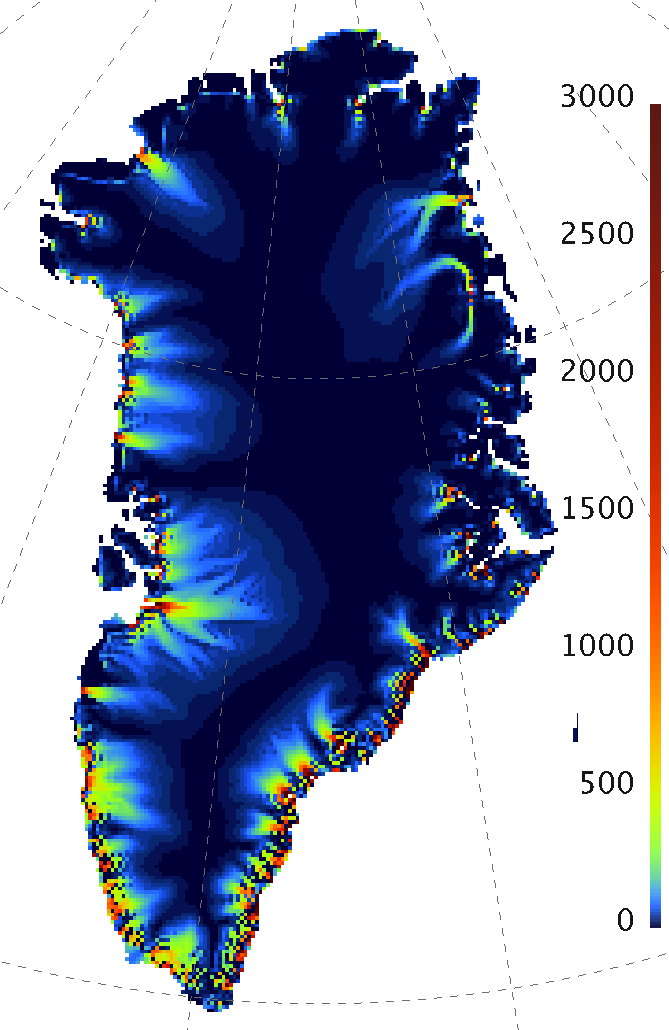
\includegraphics[width=2.in,keepaspectratio=true]{csurf}}
\caption{FIXME Model for the present-day Greenland ice sheet, based on spin-up over 125,000 model years using paleo-climate forcing.  Left: ice thickness (m).  Center: basal sliding speed (m/a).  Right: surface speed (m/a).  These are fields \texttt{thk}, \texttt{cbase}, and \texttt{csurf} from file \texttt{g10km_0.nc}.}
\label{fig:sr-spindone-map}
\end{figure}

FIXME The actual paleo-climate-driven spin-up starts from model state \texttt{g20km_steady.nc}.  We turn on three new mechanisms, climatic forcing, bed deformation, and improved stress balance.  There are two forms of climatic forcing. First, temperature offsets from GRIP core data affect the snow energy balance and thus rates of melting and runoff; the model is a simple temperature-index scheme described at the SeaRISE website.  Thereby the surface mass balance varies over time; in warm periods there is more marginal ablation.  Additionally, sea levels from the SPECMAP cores affects which ice is floating.

Significantly, we start using a more complete ice dynamics model with sliding controlled by a membrane stress balance, the SIA+SSA hybrid model described in section \ref{sec:dynamics}.  This is turned on with option ``\texttt{-ssa_sliding}''.

Also, we turn on a bed deformation model; the option is ``\texttt{-bed_def lc}''.  

These options are discussed in section \ref{sec:modeling-dynamics}.



\subsection{More runs: grid sequencing}  \label{subsect:gridseq}  

\subsection{More runs: a sliding parameter study}  \label{subsect:paramstudy}

% 9 runs:
-pseudo_plastic_q   0.0 0.25 1.0
-sia_e   1 3 10

\subsection{Going forward}  \label{subsect:forecastcaution}  Because real ice sheets, and ice sheet models too, have a ``memory'' of past climates, results of ``forecast'' runs may strongly depend on the nature of the spin-up process which create the initial conditions.  It is critical to evaluate the quality of the spunup state, for example using present-day observations of surface velocity and other fields \cite{AschwandenAdalgeirsdottirKhroulev}.  Critical thinking about a broad range of modeling hypotheses is prerequisite to building models of future behavior.


\subsection{Handling NetCDF files}\label{subsect:nctoolsintro}  PISM takes one or more NetCDF files as input, then it does some computation, and then it produces one or more NetCDF files as output.  Usually, other tools help to extract meaning from these NetCDF files, and yet more tools help with creating PISM input files or post-processing PISM output files.

Table \ref{tab:NetCDFview} lists such tools.  We frequently use \texttt{ncview}, ``\texttt{ncdump -h}'', and NCO for quick visualization, metadata examination, and command-line manipulation, respectively.  Visualization tools IDV and PyNGL are especially useful.  

To use CDO on PISM files, first run the script \texttt{nc2cdo.py}, from the \texttt{util/} PISM directory, on the file.  This fixes the metadata so that CDO will understand the mapping.

Regarding the creation of input files for PISM, see the section \ref{sec:bootstrapping-format} and table \ref{tab:modelhierarchy} for ideas about the data necessary for modeling.

\newcommand{\netcdftool}[1]{#1\index{NetCDF!tools!#1}}
\begin{table}[ht]
\centering
\small
\begin{tabular}{llp{0.45\linewidth}}
  \toprule
  \textbf{Tool} & \textbf{Site} & \textbf{Function} \\
  \midrule
  & \url{www.unidata.ucar.edu/software/netcdf/} & root for NetCDF information \\
  \midrule
  \netcdftool{\texttt{ncdump}} & \emph{included with any NetCDF distribution} & dump binary NetCDF as \texttt{.cdl} (text) file \\
  \netcdftool{\texttt{ncgen}} & \emph{included with any NetCDF distribution} & convert \texttt{.cdl} file to binary NetCDF \\
  \midrule
  \netcdftool{CDO} & \url{http://code.zmaw.de/projects/cdo} & = Climate Data Operators; command-line tools, including conservative re-mapping \\
  \netcdftool{IDV} & \url{http://www.unidata.ucar.edu/software/idv/} & more complete visualization \\
  \netcdftool{NCO}\index{NCO (NetCDF Operators)} & \url{http://nco.sourceforge.net/} & = NetCDF Operators; command-line tools\\
  \netcdftool{NCL} &  \url{http://www.ncl.ucar.edu} & = NCAR Command Language\\
  \netcdftool{\texttt{ncview}} & \href{http://meteora.ucsd.edu/~pierce/ncview_home_page.html}{\texttt{meteora.ucsd.edu/$\sim$pierce}} & quick graphical view \\
  \netcdftool{PyNGL} &  \url{http://www.pyngl.ucar.edu} & Python version of NCL\\
  \bottomrule
\end{tabular}
\normalsize
\caption{A selection of tools for viewing and modifying NetCDF files.}
\label{tab:NetCDFview}
\end{table}


%%% Local Variables: 
%%% mode: latex
%%% TeX-master: "manual"
%%% End: 


% LocalWords:  metadata SPECMAP paleo html IDV



\clearpage
\newpage
\section{Ice dynamics, the PISM view}\label{sect:dynamics}

\subsection{PISM design principles}\index{PISM!principles}  This section gives an overview of ice dynamics models in PISM, but first we list some organizing principles:
\begin{enumerate}
\item source code should be open, free, and works well with other free software tools,
\item science is better if done with publicly-available data,
\item numerical methods should be verifiable (i.e.~we want comparisons to exact solutions of the modeled equations),
\item shallow models are (currently) the most effective at whole ice sheet scale,
\item comparing results from a hierarchy of ice dynamics simplifications is more important than getting them from any particular set of dynamical equations,
\item everything computed diagnostically (instantaneously) is available prognostically (i.e.~it can evolve in time), and
\item climate inputs should affect ice dynamics by a well-defined interface.
\end{enumerate}

\noindent We do not claim to follow these principles perfectly, but we hope that any user can see these principles reflected in PISM and this \emph{Manual}.

Principle 1 is illustrated by our existence.  Principle 2 is illustrated by examples in sections \ref{sect:start}, \ref{sec:eismint-greenland}, and \ref{sect:ross}.  Principle 3 is addressed in section \ref{sect:verif}.  Principles 4, 5, 6, and 7 are explained and expanded next.


\subsection{Two main shallow models, SIA and SSA}\index{PISM!SIA}\index{PISM!SSA}  At each time-step of a typical PISM run, the geometry, temperature, and basal strength of the ice sheet are included into stress (momentum) balance equations to determine the velocity of the flowing ice.   The ``full'' stress balance equations, namely the (non-Newtonian) Stokes model for slowly-flowing fluids \cite{Fowler}, are themselves an inertia-free approximation of the conservation of momentum equations.  Though PISM does not solve this ``full'' model, it can numerically solve two significantly-different shallow approximations of the full stress balance equations:\begin{itemize}
\item the non-sliding shallow ice approximation (SIA)\index{SIA (shallow ice approximation)} \cite{Hutter}, which describes ice as flowing by shear in planes parallel to the geoid, with an infinitely-strong contact of ice base to bedrock, and
\item the shallow shelf approximation (SSA)\index{SSA (shallow shelf approximation)} \cite{WeisGreveHutter}, which describes a membrane-type flow of floating ice \cite{Morland}, or grounded ice which is sliding over a weak base \cite{MacAyeal,SchoofStream}.
\end{itemize}
PISM solves both the SIA and SSA equations in parallel.  Time-stepping solutions of the mass continuity and energy conservation equations are possible when using each model.

The SIA\index{SIA (shallow ice approximation)!applicability} equations are, as a rule, easier and quicker to numerically solve than the SSA, and they are also easier to parallelize.\index{parallelization!relative ease of, between SIA and SSA}  They are a ``lubrication approximation'' \cite{Fowler} which describes the shear as a local function of the driving stress of classical glaciology \cite{Paterson}.  They can confidently be applied to those grounded parts of ice sheets for which the basal ice is frozen to the bedrock, or minimally sliding, and for which the bed topography is relatively slowly-varying in the map-plane \cite{Fowler}.  These characteristics apply to the majority \emph{by area} of the Greenland and Antarctic ice sheets.  We recommend solving the SIA with a \emph{non-sliding} base because the ad hoc addition of ``sliding laws''\index{SIA (shallow ice approximation)!sliding laws} into the SIA stress balance, and especially schemes which ``switch on'' at the pressure-melting temperature \cite{EISMINT00}, have bad continuum and numerical modeling consequences \cite[appendix B]{BBssasliding}.

The SSA\index{SSA (shallow shelf approximation)!applicability} equations can confidently be applied to large floating ice shelves, which have small depth-to-width ratio and negligible basal resistance \cite{Morland,MorlandZainuddin}.  Terrestrial ice sheets also have fast-flowing grounded parts, however, called ``ice streams'' or ``outlet glaciers''.  Such features appear at the margin of, and sometimes well into the interior of, the Greenland \cite{Joughinetal2001}\index{Greenland ice sheet} and Antarctic \cite{BamberVaughanJoughin}\index{Antarctic ice sheet} ice sheets.  Describing these faster-flowing grounded parts of ice sheets requires something more than the non-sliding SIA.  One might use the full Stokes equations, or a ``higher-order'' but still shallow stress balance \cite{Blatter,Pattyn03}, but with any stress balance model one must still specify an appropriate sliding boundary condition.  To address these faster-flowing parts, one may apply the SSA equations with additional basal resistance terms to model fast-flowing and sliding grounded ice.  This was demonstrated for the Siple Coast ice streams of Antarctica by MacAyeal\index{MacAyeal, Doug} \cite{MacAyeal} using a linearly-viscous model for the underlying till.  A free boundary problem with the same (SSA) balance equations is the Schoof\index{Schoof, Christian} \cite{SchoofStream} model of ice streams, in which ice streams appear where there is plastic basal till failure \cite{Paterson}.

Both the SIA and SSA models are \emph{shallow} approximations.  That is, the respective partial differential equations are derived from the Stokes equations by different small-parameter arguments, both based on a small depth-to-width ratio for the ice sheet.  For the small-parameter argument in the SIA case see \cite{Fowler}.  For the corresponding SSA argument, see \cite{WeisGreveHutter} or the appendices of \cite{SchoofStream}.  See \cite{SchoofHindmarsh} on connections between these shallowest models and ``higher order'' models.  For additional discussion of continuum equations for ice sheets, and for more on the physical motivation behind shallow modeling, see \cite{GreveBlatter2009}.

In PISM the SSA may be used as a ``sliding law'' for grounded ice which is otherwise modeled by the non-sliding SIA.  The resulting hybrid model is recommended for many purposes \cite{BBssasliding,BKAJS}.  This role for the SSA is in addition to its obvious role in ice shelf modeling.  In brief, our concept for grounded ice is that we must balance the membrane stresses which become important anywhere there is significant sliding.  These stresses are especially important near spatial (and temporal) changes in basal strength.  Similar concerns at the ``grounding line'', where ice flows into a floating ice shelf, also suggest that membrane stresses on the grounded side of the grounding line are worth including.

By default, PISM does not numerically solve the SSA because any such solution must go with a conscious user choice about basal strength.  The user must both use one of two options to turn on the SSA (section \ref{subsect:ssacontrol}) and also make choices in input files and runtime options about basal strength (section \ref{subsect:basestrength}).


\subsection{A hierarchy of simplifying assumptions for ice flow}\label{sec:model-hierarchy}\index{PISM!hierarchy of simplifying assumptions}   Table \ref{tab:modelhierarchy} describes a hierarchy of models which are implemented in PISM or are planned.  This hierarchy is listed in order of increasing effectiveness in modeling grounded ice sheets with fast flow features.  It is also listed in order of increasing need for data to serve as boundary and initial conditions, an important consideration for the scientific user.

\begin{table}[ht]
\caption{Hierarchy of current and planned flow models in PISM, for the grounded parts of ice sheets, from most to fewest simplifying assumptions \emph{and} from least to greatest need for boundary data.  The \emph{italicized} models are planned for future versions of PISM but are not implemented in \texttt{stable0.3}.}\label{tab:modelhierarchy} 
\small
\begin{tabular}{p{0.25\linewidth}p{0.35\linewidth}p{0.3\linewidth}}\hline
\textbf{Model} & \textbf{Assumptions [references]} & \textbf{Needed initial/boundary data} \\ \hline
\emph{perfectly-plastic ice} \tiny[planned]\small & \emph{steady state}; all points in the ice have shear stresses at or below a pre-determined ``yield stress'' & bed elevation, chosen location for margin \\
\emph{balance velocities} \tiny[planned]\small & \emph{steady state}; ice flows down surface gradient \cite{JoughinetalGrBal97} & surface mass balance, ice  thickness, bed elevation \\
\textsc{isothermal SIA} & non-sliding lubrication flow, fixed softness \cite{BLKCB,EISMINT96} & same, with time-dependence \\
\textsc{thermo-coupled SIA} & non-sliding lubrication flow, temperature-dependent softness \cite{BBL,EISMINT00} & same, plus surface temperature,  geothermal flux \\
\textsc{polythermal SIA} & same, but allowing liquid water in the temperate ice matrix and conserving energy more completely \cite{AschwandenBlatter,Greve} & same, plus surface liquid water fraction if available \\
\textsc{SIA + SSA hybrid} & SSA as a sliding law for thermo-coupled SIA \cite{BBssasliding} & same, plus basal layer (till) strength \\
\emph{Blatter-Pattyn} \tiny[planned]\small & ``higher-order'', bridging stresses \cite{Blatter,Pattyn03,SchoofCoulombBlatter} & same \\ \hline
\end{tabular}
\normalsize
\end{table}

As an additional row one might list ``full Stokes'' in Table \ref{tab:modelhierarchy}.  That stress balance is \emph{not} planned for PISM at any time, however, as its numerical solution requires a fundamentally different computational architecture.

It makes sense to also talk about an \emph{ice shelf} model hierarchy, and even about a special hierarchy of models for the transition from grounded to floating ice \cite{SchoofMarine1}, but this would take us too far afield.  Currently, ice shelves should always be modeled by the SSA equations in PISM.


\subsection{Evolutionary versus diagnostic ice shelf modeling} \label{subsect:basicmodes}\index{PISM!evolution run}\index{PISM!diagnostic run}    The main goal of a numerical ice sheet model like PISM is to be a dynamical system which evolves over time as similarly as possible to the modeled ice sheet.  Such a goal assumes one has the right climate inputs and parameter choices at each time step.  For predictive purposes, such a goal also assumes one starts with the right initial conditions, adequately describing the present state of the ice sheet.  (In fact this last assumption is rarely satisfied and heuristics must be used to minimally-initialize an ice sheet model, before a possible stage of paleo-climate driven spinup; see section \ref{sect:boot}.)

Underlying an ice sheet model like PISM are evolution-in-time partial differential equations.  PISM solves these by taking small time steps.  ``Small'' time steps vary from hundredths to many model years, depending primarily on both grid resolution and modeled ice flow speed.  Time steps are chosen adaptively in PISM, according to the stability criteria of the several numerical methods.  We will describe this usual time-stepping behavior as an ``evolution run.''

However, much ice flow modeling, especially of streams and shelves, uses only instantaneous ``diagnostic'' solution of the partial differential equations which determine the velocity field.  The existence of such ``instantaneous'' velocity fields follows from the slowness of the ice, which implies that inertia can be neglected in the stress balance \cite{Fowler}.  The goal of a ``diagnostic run'' is usually to compute the velocity field, including the instantaneous rate of surface movement in particular.  This will be our definition of ``diagnostic run'' from now on.  (Especially for grounded ice, making diagnostic runs may be the ``forward model'' step in inverting surface velocities for basal strength.  But again that would take us far afield.)

Sections \ref{sec:eismint-greenland} and \ref{sect:ross} are examples which illustrate the evolutionary and diagnostic modeling modes of PISM.  The first of these describes time-stepping evolution models for the Greenland ice sheet, while the second describes a diagnostic SSA model for the Ross ice shelf.

\subsection{Climate inputs and their separation from ice dynamics}
\label{sec:climate-inputs}  This section applies the seventh PISM organizing principle above (section \ref{sect:dynamics}): \emph{climate inputs affect ice dynamics by a well-defined interface}.

Because PISM's job is to approximate ice flow, its world view is centered around ice dynamics.  The boundary conditions required to model dynamics, and the corresponding interfaces, are necessarily ``ice-centric'' in our description here, but we believe there is no actual constraint on the nature of the other climate models which could be coupled to PISM.

Figure~\ref{fig:climate-inputs} is an illustration emphasizing that the ice sheet has a top surface interface (green dashed line in the figure) separating it from a surface processes (snow, firn, melt, runoff, \dots processes) layer.  This latter layer of modeled processes is assumed in PISM to cover the whole surface of the ice, including ablation areas, and even ice-free bedrock.

\begin{figure}
  \centering
  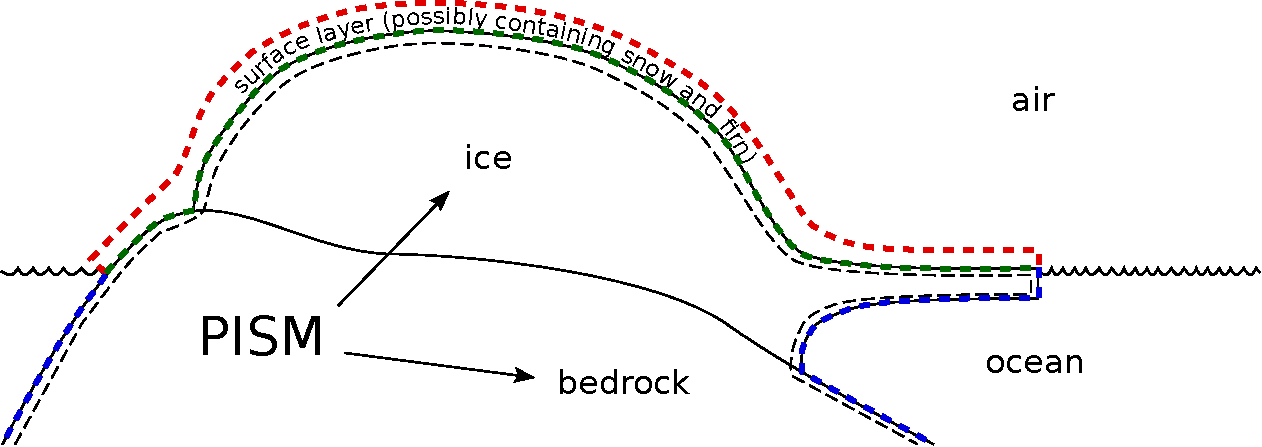
\includegraphics[width=5in]{figs/climate-cartoon-new.pdf}
  \caption{PISM's view of interfaces between an ice sheet and the outside world}
  \label{fig:climate-inputs}
\end{figure}

\begin{table}[h]
  \centering
  \begin{tabular}{p{0.35\linewidth}p{0.55\linewidth}}\\
    \hline
    \textbf{Boundary} & \textbf{Necessary conditions}\\
    \hline
    Top ice surface (below firn) (\textcolor{green}{green})& Ice temperature (or enthalpy) and mass flux into the ice\\
    Bottom surface of the thermal bed layer (not shown) & Geothermal flux\\
    Ice shelf basal surface (\textcolor{blue}{blue})& Mass flux into the ocean and ice boundary temperature\\
   \hline
  \end{tabular}
  \caption{Boundary conditions required by PISM's ice dynamics core; see figure
  \ref{fig:climate-inputs}}
  \label{tab:ice-dynamics-bc}
\end{table}

Regarding the base of the ice, as described in section \ref{subsect:beddef} PISM also includes an optional bed deformation component approximating the movement of the Earth's crust and upper mantle in response to changing ice load.   Furthermore the temperature of the layer of bedrock in contact with grounded ice is included in the conservation of energy model.  In this sense everything below the black dashed line (i.e.~ice and bedrock) is ``owned'' by PISM, which adds two more boundary interfaces for the ice dynamics core: sub-ice-shelf/ocean (shown in blue) and the bottom of the bedrock thermal layer (not shown).

Table \ref{tab:ice-dynamics-bc} lists boundary conditions required at
interfaces mentioned above.\footnote{This is a somewhat simplified view  corresponding to a ``generic'' PISM run.   See section \ref{sec:model-hierarchy} for details.}

The PISM ice dynamics core would like to be able to get these fields directly from observations or measurements, or directly from a GCM.  In many realistic modeling situations, however, PISM code must be used for all or part of the surface processes modeling necessary to provide the ice-dynamics core with the ``right'' fields.  Due to differences in model resolutions and required down-scaling, this need for some PISM-based boundary-processes modeling includes cases where PISM is coupled to a GCM.  In the kind of ``offline'' runs described in this \emph{Manual}, boundary processes are modeled, even if trivially.

Thus, in able to use the data that \emph{is} available, an ice-sheet model has to
have additional components that are responsible for modeling surface (snow)
processes or sub-shelf/ocean interaction.  These components might be very minimal, merely turning data that we already have into data in the right units and with the right metadata, so that PISM knows what to do with it, for example.

Thus we have PISM's design: the ice-dynamics-and-earth-deformation PISM
core does not contain any parameterization or other model for boundary mass or
energy balance.  These boundary parameterizations and models are present in the PISM source code, however, as instances of \emph{PISMComponent} classes.  This simplifies customizing and debugging PISM's climate
inputs, promotes code reuse.  It isolates the code that needs to be changed to
couple PISM to a climate model.

Users wishing to customize PISM's climate inputs should see the \emph{PISM
  Source Browser}, e.g.~at
\url{http://www.pism-docs.org/dev/doxy/html/index.html} and the documentation
of \emph{PISMSurfaceModel}, \emph{PISMAtmosphereModel} and
\emph{PISMOceanModel} therein.  Also, section \ref{sec:eismint-greenland} describes a
modeling example using a non-standard air temperature parameterization. Looking
at \texttt{pgrn.cc} and \texttt{pgrn_atmosphere.cc} may be a reasonable
start.

Note that figure~\ref{fig:climate-inputs} includes an interface that was not
mentioned yet, the one between the surface layer and the air (red dashed line).
Unlike the ones listed in table~\ref{tab:ice-dynamics-bc}, this interface
\emph{may not even be present in some PISM configurations:} the ice dynamics
core of PISM only ``knows'' about mediums bordering ice and bedrock. A pair
consisting of a \emph{PISMSurfaceModel} and a \emph{PISMOceanModel} may be
hiding anything from a nearly trivial parameterization of ice surface
temperature plus surface and sub-shelf mass fluxes to a GCM of great
complexity.

Figure~\ref{fig:climate-input-data-flow} illustrates the corresponding data
flow \emph{into} the PISM core; the data flow in the other direction depends on
particular modeling choices.

This figure requires an explanation: a ``modifier'' in this context is an
adjustment of climate inputs that can be used with different climate
choices.  Using ice-core-derived air temperature offsets to model the space-time distribution of paleo surface temperature is an example.  Note that PISM has a generic ``forcing'' mechanism that can be paired with another model. Please see section \ref{sec:boundary-models} for
a list of climate components included in PISM source code and other details.

\begin{figure}
  \centering
  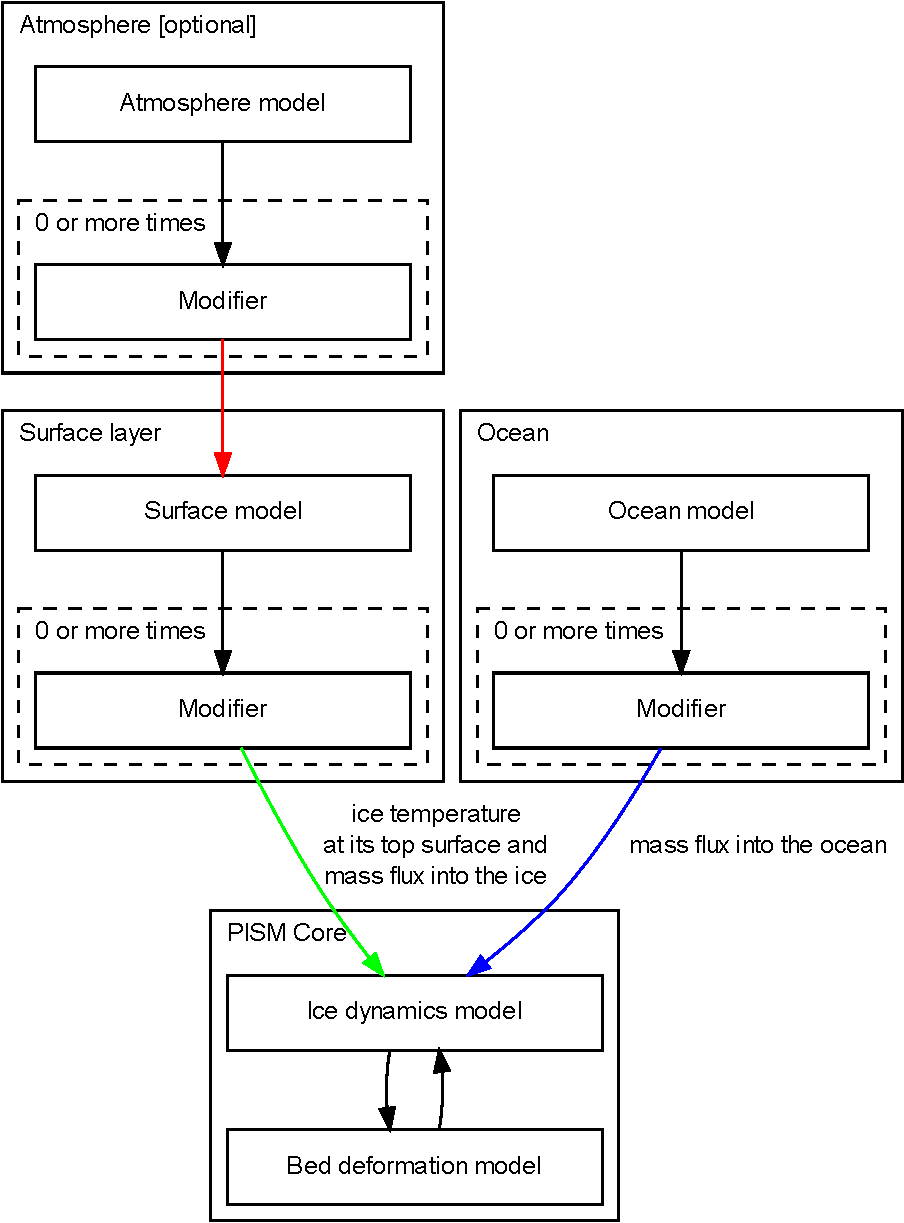
\includegraphics[width=5in]{figs/data-flow.pdf}
  \caption{PISM climate input data flow. Colored arrows correspond to interfaces in
    figure \ref{fig:climate-inputs}.}
  \label{fig:climate-input-data-flow}
\end{figure}

Why describe this structure here? On the one hand, some users may be interested
in coupling PISM to other models. On the other hand, the PISM authors do not
claim expertise in modeling atmosphere, ocean, or even snow processes.   So the
separation has a code-reliability purpose. Indeed PISM users need to know that
they are ultimately responsible for providing the climate inputs they intend.
The auxiliary tool \texttt{pclimate}, described in subsection
\ref{subsect:pclimate}, is intended to help users observe the climate inputs
they have chosen, without involving ice dynamics at all.

\clearpage
\newpage
\section{Initialization and bootstrapping}\label{sect:boot}  

\subsection{``Initialization from a saved model state''}  This phrase\index{initialization!from saved model state} has a simple meaning in PISM.  If a previous PISM run has saved a NetCDF file using ``\texttt{-o}'' then that file will contain complete initial conditions for continuing the run.  The output file from the last run can be loaded with ``\texttt{i}'':\index{pisms}

\begin{verbatim}
$ pisms -eisII A -y 100 -o foo.nc
$ pisms -eisII A -i foo.nc -y 100 -o bar.nc
\end{verbatim}
\smallskip

Note that simplified-geometry experiments (section \ref{sect:simp}) and verification tests (section \ref{sect:verif}) do not need input files at all because they initialize from formulas in the source code.  They can be continued from saved model states using \texttt{-i}.  As in the above example, however, specifying the simplified geometry experiment or verification test \emph{is} necessary, so that the run can continue with the climate inputs for that experiment or test.  For example, based on the above \verb|pisms| runs, it is valid to do ``\verb|$ pismr -i foo.nc -y 100 -o bar.nc|'' but the climate and other parameters us PISM default values, and thus are not (necessarily) the values specified in EISMINT II.

As a technical but important note about saved states, a PISM run with \texttt{-ssa_floating_only} or \texttt{-ssa_sliding}
also saves the last SSA velocities to the output file, in variables 
\texttt{ubar_ssa} and \texttt{vbar_ssa}.  A \texttt{ssa_velocities_are_valid} global
attribute shows if the data present in these variables is valid.  The presence
of these velocities adds efficiency in restarting.  If you want a PISM restart to
ignore these velocities use \texttt{-dontreadSSAvels}.

\subsubsection*{\texttt{-i} file format}
PISM produces CF-1.4 compliant NetCDF\index{PISM!NetCDF file format}\index{NetCDF} files.  The easiest way to learn the output format \emph{and} the \texttt{-i} format is to do a simple run and then look at the metadata in the resulting file, like this:
\begin{verbatim}
$ pisms -eisII A -y 10 -o foo.nc
$ ncdump -h foo.nc | less
\end{verbatim}

Note that variables have a \texttt{pism_intent}\index{PISM!\texttt{pism_intent} attribute} attribute.  When that attribute is \texttt{diagnostic}, the variable can be deleted from the file without affecting whether PISM can use it as a \texttt{-i} input file.  Variables with \texttt{pism_intent} = \texttt{model_state}, by contrast, must be present for use with \texttt{-i}.

Regarding the automatically produced time variable, which has a \texttt{units} attribute like \texttt{"years since 1-1-1"}, note that CF metadata conventions require using a reference date in the units string of a time (\texttt{t}) variable.  PISM completely ignores this reference date.


\subsection{``Bootstrapping''} 
\optsection{Bootstrapping}
\optseealso{Grid}

This phrase\index{bootstrapping}\index{initialization!by bootstrapping} means starting a modeling run with less than sufficient data, and letting the model fill in needed values according to heuristics.  These heuristics are applied before the first time step is taken, so they are part of an initialization process.  Bootstrapping uses the option \fileopt{boot_from}.

The need for an identified stage like ``bootstrapping'' comes from the fact that initial conditions, for the evolution equations describing an ice sheet, are not typically observable.  As a principal example of this problem, these equations require the temperature within the ice at the time the run is started.  Glaciological observations, specifically remote-sensed observations which cover a large fraction or all of an ice sheet, never include this temperature field in practice.

Instead, evolutionary ice sheet modeling necessarily does something like this to get ``reasonable'' initial fields within the ice: \begin{enumerate}
\item start only with observable quantities like surface elevation, ice thickness, and ice surface temperature,
\item ``bootstrap'' as defined here, using heuristics to fill in temperatures at depth and to give a preliminary estimate of the basal sliding condition, and thus of the three-dimensional velocity field, and
\item \emph{either} do a long run holding the current geometry and surface temperature steady,  to evolve toward a ``more physical'' steady state which will have compatible temperature field, velocities, and age field,
\item \emph{or} do a long run using an additional spatially-imprecise historical record from an ice core or a sea bed core (or both), to apply forcing to the surface temperature or sea level (for instance), but with the same functional result of filling in a temperature, velocity, and age.
\end{enumerate}

The heuristics used by PISM are, for now, only documented in the source code file \texttt{src/base/iMbootstrap.cc}.

When using \fileopt{boot_from} you will need to specify both grid dimensions (using \t{Mx}, \t{My} and \t{Mz}) and the height of the computational box for the ice with \t{Lz}.  The data read from the file can determine the horizontal extent of the model, if options \t{Lx}, \t{Ly} are not set.  The additional specification of vertical extent by \texttt{-Lz} is reasonably natural because realistic data used in ``bootstrapping'' are two-dimensional.  Not specifying all four options \texttt{-Mx}, \texttt{-My}, \texttt{-Mz}, \texttt{-Lz} \emph{when bootstrapping with} \texttt{-boot_from} is an error.

Subsection \ref{sec:eismint-greenland} shows bootstrapping for the EISMINT-Greenland intercomparison.

\subsubsection*{\texttt{-boot_from} file format}
\label{sec:bootstrapping-format}  Allowed formats for a bootstrapping file are relatively simple to describe. 
\begin{enumerate}
\item The NetCDF dimensions \texttt{x} and \texttt{y} and corresponding variables must be present and have the meanings of projection X coordinate and projection Y coordinate.
\item Coordinate variables \texttt{x} and \texttt{y} have to be strictly increasing.
\item All three-dimensional variables (depending on \texttt{x,y,z} or \texttt{x,y,zb}) will be ignored in bootstrapping.
\item The \texttt{standard_name} attribute is used to identify a variable, so the names of variables do not need to match the corresponding variables in a PISM output file.
\item PISM expects all the input fields (NetCDF variables) to be in MKS \emph{or} to have the units specified using the \texttt{units} attribute.  PISM uses a library called UDUNITS\index{PISM!uses UDUNITS when reading NetCDF files}\index{UDUNITS} to convert data present in an input file to MKS.   This means that having ice thickness in feet or kilometers, or temperature in Celsius for example, is allowed.
\item Any two-dimensional variable (depending on \texttt{x,y}) may be missing.  For those missing variables some heuristic will be applied.  See table \ref{tab:modelhierarchy} for a sketch of the data necessary for bootstrapping, and \texttt{src/base/iMbootstrap.cc} for all further details.
\item Surface elevation is ignored if present.  Users with surface elevation and bed elevation data should produce an ice thickness variable, with \texttt{standard_name} = \texttt{land_ice_thickness} for bootstrapping.  The bed elevation (topography) is read by \texttt{standard_name} = \texttt{bedrock_altitude}.
\end{enumerate}

\subsection{For programmers deriving/modifying PISM:  Initialization sequence}  As described already, there are three ways to start PISM,\begin{itemize}
\item executables \texttt{pisms} and \texttt{pismv} initialize simplified-geometry experiments and verification tests, respectively, from formulas in the source code,
\item \texttt{-i} reads a previously-saved PISM model state in NetCDF form, and
\item \texttt{-boot_from} reads a NetCDF file and uses heuristics to fill in needed fields.
\end{itemize}
As a consequence of these options, and generally from the complexity of getting a computation started on a parallel computer, we observe that initializing PISM is one of the most error-prone parts of maintaining it.

Thus initialization sequence is also an error-prone part of writing a derived class of \texttt{IceModel} to modify PISM's function.  The reader interested in doing so should see method \texttt{IceModel::init()} and also view the flow chart in \texttt{doc/initialization-sequence.png}.  Note that \texttt{init()} is \emph{not} \texttt{virtual}.  Derived classes can redefine the several methods which are called by \texttt{init()}, which are \texttt{virtual}.


\clearpage\newpage

\section{Making Modeling Choices}
\label{sec:modeling-choices}

\subsection{Computational box} \label{subsect:coords}
\optsection{Computational box}
\optseealso{Grid}

PISM does all simulations in a computational box\index{PISM!computational box} which is rectangular in the PISM coordinates.

The coordinate system has horizontal coordinates $x,y$ and a vertical coordinate $z$.  The $z$ coordinate is measured positive upward from the base of the ice and it is exactly opposite to the vector of gravity.  The surface $z=0$ is the base of the ice, however, and thus is usually not horizontal in the sense of being parallel to the geoid.   The surface $z=0$ is the base of the ice both when the ice is grounded and when the ice is floating.

Bed topography is, of course, allowed.  In fact, when the ice is grounded, the true physical vertical coordinate $z'$, namely the coordinate measure relative to a reference geoid, is given by $z'=z+b(x,y)$ where $b(x,y)$ is the bed topography.  The surface $z'=h(x,y)$ is the surface of the ice.

In the grounded case the equation $h(x,y)=H(x,y)+b(x,y)$ always applies if $H(x,y)$ is the thickness of the ice.  In the floating case, the physical vertical coordinate is $z'=z-(\rho_i/\rho_s) H(x,y)$ where $\rho_i$ is the density of ice and $\rho_s$ the density of sea water.  Again $z=0$ is the base of the ice, which is the surface $z' = -(\rho_i/\rho_s) H(x,y)$.  The surface of the ice is $h(x,y) = (1-\rho_i/\rho_s) H(x,y)$.  All we know about the bed elevations is that they are below the base of the ice when the ice is floating.  That is, the \emph{flotation criterion} $-(\rho_i/\rho_s) H(x,y) > b(x,y)$ applies.

The computational box can extend downward into the bedrock.  As $z=0$ is the base of the ice, the bedrock corresponds to negative $z$ values regardless of the sign of its true (i.e.~$z'$) elevation.

The extent of the computational box, along with its bedrock extension downward, is determined by four numbers \t{Lx}, \t{Ly}, \t{Lz}, and \t{Lbz} (see Figure \ref{fig:rectilinearbox}.).  The first two of these are half-widths and have units of kilometers when set by options or displayed.  The extent of the computational box for the ice and bedrock is directly controlled by the following options. 

\begin{center}
  \begin{tabular}{llp{0.7\linewidth}}
    \\\hline
    \textbf{Option} & \textbf{Meaning}
    \\\hline
    \txtopt{Lx}{(km)} & Half-width of the computational domain (in the $x$-direction) \\
    \txtopt{Ly}{(km)} & Half-width of the computational domain (in the $y$-direction) \\
    \txtopt{Lz}{(meters)} & Height of the computational domain in the ice \\
    \txtopt{Lbz}{(meters)} & Depth of the computational domain in the bedrock thermal layer
    \\\hline
  \end{tabular}
\end{center}

\begin{figure}[ht]
\centering
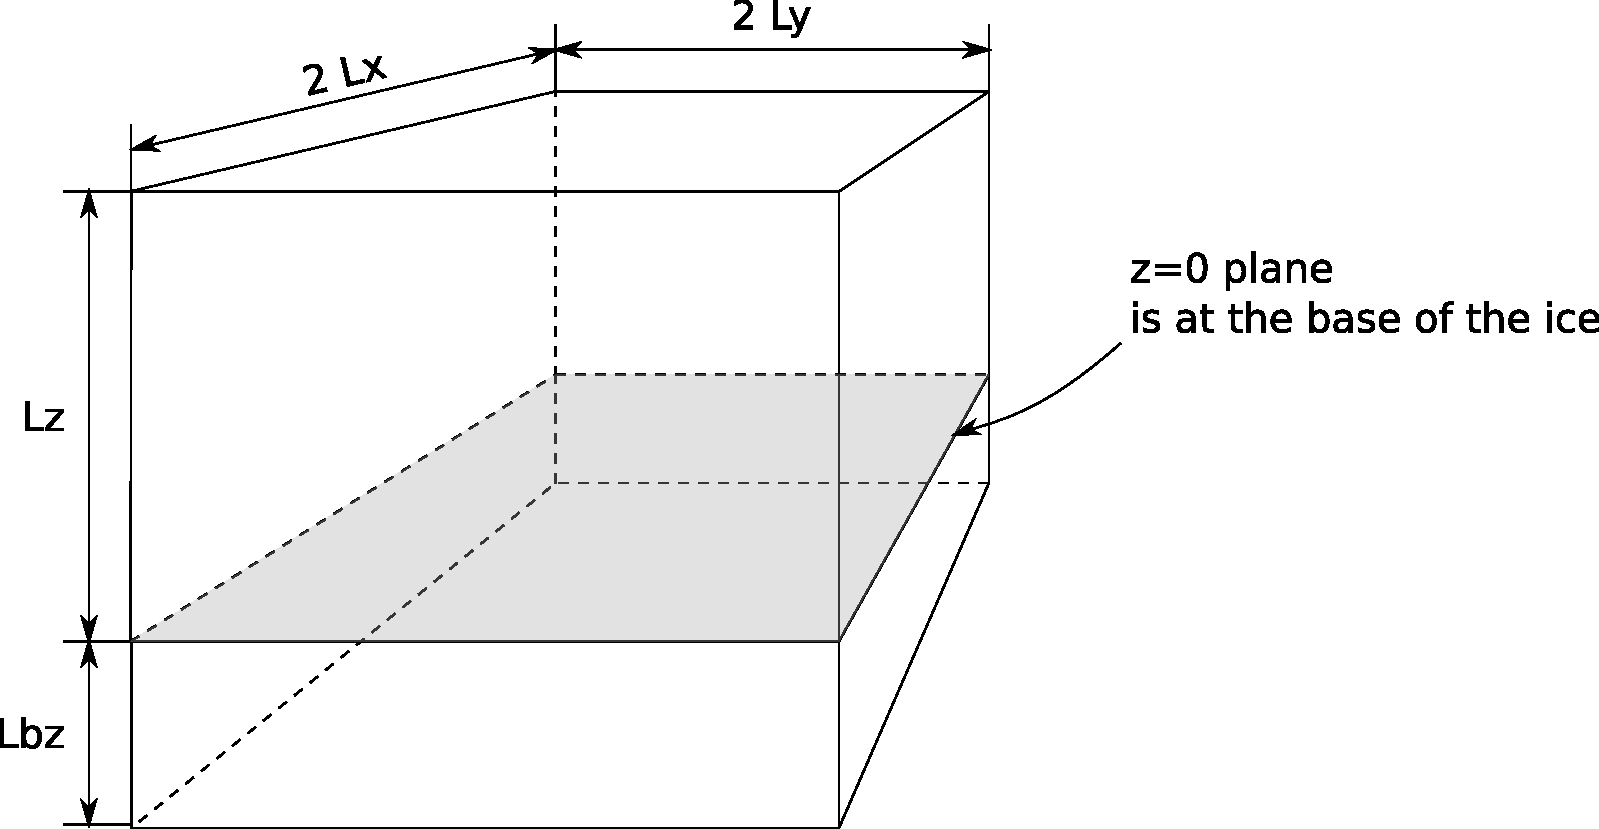
\includegraphics[width=4.0in,keepaspectratio=true]{rectilinearbox}
\caption{PISM's computational box.}
\label{fig:rectilinearbox}
\end{figure}


\subsection{Spatial grid}
\label{subsect:grid}
\optsection{Grid!space}

The PISM grid\index{PISM!grid} covering the computational box is equally spaced in horizontal ($x$ and $y$) directions.  Vertical spacing is quadratic by default (see below) but optionally a different spacing scheme can be chosen.  (Choose with options \txtopt{z_spacing}{[quadratic, equal]} and \txtopt{zb_spacing}{[quadratic, equal]}.)

The grid is described by four numbers, namely the number of grid points \texttt{Mx} in the $x$ direction, the number \texttt{My} in the $y$ direction, the number \texttt{Mz} in the $z$ direction within the ice, and the number \texttt{Mbz} in the $z$ direction within the bedrock thermal layer.  These are specified by options \intextoption{Mx}, \intextoption{My}, \intextoption{Mz}, and \intextoption{Mbz}, respectively. The defaults are 61, 61, 31, and 1, respectively.

Note that \texttt{Mx}, \texttt{My}, \texttt{Mz}, and \texttt{Mbz} all indicate the number of grid \emph{points}.  The number of grid \emph{spaces} are one less, thus 60, 60, 30, and 0 in the default case.  The lowest grid point in a column of ice, at $z=0$, coincides with the highest grid point in the bedrock, so \texttt{Mbz} must always be at least one and \texttt{Mbz}$>1$ is required to use the bedrock thermal model.  Note that this option is unrelated to the bed deformation model (glacial isostasy model); see option \texttt{-bed_def} for that.

In the quadratic case, the spacing near the ice/bedrock interface is about four times finer than it would be with equal spacing for the same value of \texttt{Mz} (or \texttt{Mbz}), while the spacing near the top (or bottom) is correspondingly coarser. For a detailed description of the spacing of the grid, see the documentation on \texttt{IceGrid::compute_vertical_levels()} in the PISM class browser.

When a thermal bedrock layer is used, the distance \texttt{Lbz} is controlled by the \texttt{-Lbz} option.

If one initializes PISM from a saved model state using \t{i} then the input model state controls the parameters \t{Mx}, \t{My}, \t{Mz}, and \t{Mbz}.  For instance, the command

\begin{verbatim}
$  pismr -i foo.nc -y 100
\end{verbatim}

\noindent should work fine if \texttt{foo.nc} was a valid PISM model file.  The command

\begin{verbatim}
$  pismr -i foo.nc -Mz 201 -y 100
\end{verbatim}

\noindent will give a warning that ``\texttt{PISM WARNING: ignoring command-line option '-Mz'}'' because \texttt{-i} input files take precedence.

Otherwise, one is allowed to specify the grid when PISM is started.  In particular, the user should specify the grid when using \texttt{-boot_from} or when initializing a simplified-geometry experiment or a verification test, though defaults are generally present in the latter cases.  See sections \ref{sect:start} and \ref{sect:boot} for examples and explanation.

\subsection{Model time}
\label{sec:time}
\optsection{Grid!time}

The following command-line options control PISM time.

\begin{tabular}{lp{0.8\linewidth}}\\
\hline
\textbf{Option} & \textbf{Meaning}\\
\hline
\txtopt{y}{(years)} & Number of model years to run.\\
\txtopt{ys}{(years)} & Model year at which to start the run.  Also resets the model time, ignoring any time in the input file.\\
\txtopt{ye}{(years)} & Model year at which to end the run.\\
\hline
\end{tabular}

The default value for the end year is the start year (\texttt{-ys} or initialized model time from file) plus the default or given (\texttt{-y}) run length.  If both \texttt{-ys} and \texttt{-ye} are used then the run length is set to the difference.  Using all three of \texttt{-ys}, \texttt{-y} and \texttt{-ys} is not allowed.


\subsection{Diagnostic computations}  As a diagnostic example, consider the second of these two runs:

\begin{verbatim}
pisms -y 200e3 -o eisIIA200k.nc
pismr -i eisIIA200k.nc -y 0 -o eisIIA200k_diag.nc -o_size big
\end{verbatim}

\noindent The result of this zero-length, ``\texttt{-y 0}'', run is a NetCDF file \texttt{eisIIA200k_diag.nc} which contains the full three-dimensional velocity field in the scalar NetCDF variables \texttt{uvel}, \texttt{vvel}, and \texttt{wvel}, as well as many other variables.

This diagnostic mode is most frequently associated to the modeling of ice shelves and ice streams.  Subsection \ref{sect:ross} describes using \texttt{pross} to model the Ross ice shelf \cite{MacAyealetal}.  Verification tests I and J, section \ref{sect:verif}, are diagnostic calculations using the SSA.

Note that the NetCDF model state saved by PISM at the end of an \emph{evolution} run does not, by default, contain the three-dimensional velocity field.  Instead, it contains just the variables which are needed to restart the run, especially the ice geometry and temperature field.  One can also force PISM to save all the supported diagnostic quantities at the end of a time-stepping run using the option \texttt{-o_size big}.


\subsection{Computing ice age} \label{subsect:age}
\optsection{Computing ice age}

By default, PISM does not compute the age of the ice\index{PISM!modeling the age of the ice} because it does not directly impact ice flow using the default flow laws.   It is very easy to turn on.  Just set \intextoption{age}.

\subsection{Setting up PISM boundary (atmosphere, surface and ocean) models}
\label{sec:boundary-models}

Setting up PISM's boundary models requires selecting one model of each kind and zero or more ``model modifiers''; selected models and modifiers are chained as in Figure~\ref{fig:climate-input-data-flow}. Command-line options \texttt{-atmosphere}, \texttt{-surface} and \texttt{-ocean} take a comma-separated list of keywords as an argument; the first keyword \emph{has} to correspond to a model, the rest can be modifiers. Any of these options can be omitted to use the default atmosphere, surface or ocean model, although using a modifier requires specifying a model.

For example,
\begin{verbatim}
$ pismr -i foo.nc -atmosphere searise_greenland,forcing \
        -dTforcing delta_T.nc -surface pdd
\end{verbatim}%$
chooses a combination of SeaRISE-Greenland atmosphere model (see below),  ice-core derived temperature forcing, a PDD local surface mass balance model, and a default (constant) ocean model.

Each of PISM boundary model types currently has one ``modifier'' available; the corresponding keyword is \texttt{forcing}. Please see below for details.

\begin{enumerate}
\optsection{Climate (boundary) models!\texttt{-atmosphere} [searise_greenland, constant, temp_lapse_rate, forcing]}
\item \textbf{PISM atmosphere models.}
\begin{itemize}
  \item \emph{SeaRISE-Greenland} (\texttt{searise_greenland}, the default)

    This atmosphere model implements a longitude, latitude and elevation dependent near-surface air temperature parameterization and a cosine yearly cycle described in \cite{Faustoetal2009} and uses a constant in time ice-equivalent snow precipitation field (in units of thickness per time, variable \texttt{snowprecip}) that is read from an input file.

    The parameterization is controlled by configuration parameters with the \texttt{snow_temp} prefix.

    In addition to the temperature parameterization it implements the SeaRISE-Greenland formula for paleo-precipitation from present; a 7.3\% change of precipitation rate for every one degree Celsius of temperature change \cite{Huybrechts02} (turn on using the \intextoption{paleo_precip} option).

    Please see \url{http://websrv.cs.umt.edu/isis/index.php/Model_Initialization#Greenland} for details.

    It expects variables \texttt{snowprecip}, latitude and longitude to be present in an input file.

 \item \emph{Constant in time} (\texttt{constant})

    This atmosphere model reads the snow precipitation (variable \texttt{snowprecip}) and the mean annual near-surface air temperature (variable \texttt{temp_ma}) and provides them to a surface model.
  \item \emph{Constant precipitation using a temperature lapse rate} (\texttt{temp_lapse_rate})
    
    This atmosphere model also uses a constant snow precipitation field (\texttt{snowprecip}) and requires the mean annual near-surface air temperature (\texttt{temp_ma}) to be present in an input file. In addition to this, it dynamically corrects air temperature using a location-independent elevation lapse rate specified using the \intextoption{lapse_rate} command-line option (in units of degrees Celsius per meter).
 \end{itemize}

  The atmosphere \texttt{forcing} modifier implements temperature forcing using scalar offsets and also a mechanism applying precipitation and mean annual temperature anomalies.
  \begin{itemize}
  \item \fileopt{dTforcing} specifies a file containing scalar temperature offsets (variable \texttt{delta_T}), 
  \item \fileopt{anomaly_temp_ma} specifies a file containing spatially-variable mean annual near-surface air temperature anomalies (variable \texttt{temp_ma_anomaly}), and
  \item \fileopt{anomaly_precip} specifies a file containing spatially-variable ice-equivalent precipitation anomalies (in units of thickness per time, variable \texttt{snowprecip_anomaly}).
  \end{itemize}

  Options \texttt{-anomaly_temp_ma} and \texttt{-anomaly_precip} can be used to set up a PISM run using a GCM output, essentially achieving one-way coupling.

  Note that only one air temperature forcing mechanism can be used at any time.

\optsection{Climate (boundary) models!\texttt{-surface} [simple, constant, pdd, forcing]}
\item \textbf{PISM surface (snow) process models}

\begin{itemize}
  \item \emph{The ``invisible'' model} (\texttt{simple}, the default)

    This is the simplest ``surface model'' available in PISM. Its job is to re-interpret  precipitation as mass flux into the ice and mean annual near-surface air temperature as the temperature of the ice at the ice surface (below firn) (see \cite{Hock05}, for example). This implies that there is no melt as long as the precipitation field  is non-negative.

    However primitive it may be, this model can be useful; modeling Antarctica is one example.
  \item \emph{Constant in time} (\texttt{constant})

    This surface model reads constant in time top surface boundary conditions and provides them to the ice dynamics model (see table \ref{tab:ice-dynamics-bc}). When PISM is used with this model, variables \texttt{artm} (ice temperature at the ice surface but below firn) and \texttt{acab} (top surface mass flux into the ice) are expected to be present in an input file.

    Note: this surface model \emph{ignores}  the atmosphere model selection made using the \texttt{-atmosphere} option.

  \item \emph{Local mass balance (PDD)} (\texttt{pdd}) \index{positive degree day model} \index{PDD (positive degree day model)} \index{PISM!default positive degree day model} 

   The default PDD used by PISM, turned on by option \texttt{-surface pdd}, is based on \cite{CalovGreve05} and EISMINT-Greenland intercomparison (section \ref{sec:eismint-greenland} and \cite{RitzEISMINT}). It also implements latitude- and mean July temperature dependent ice and snow factors using formulas in \cite{Faustoetal2009}.

   Our PDD implementation is meant to be used with an atmosphere model implementing a cosine yearly cycle such as \texttt{searise_greenland}, but is not restricted to parameterizations like this one. A PDD generally adds ``white noise'' to the seasonal cycle to simulate additional daily variability associated to the vagaries of weather.  This additional random variation is quite significant, as the seasonal cycle may never reach the melting point but that point may be reached with some probability, in the presence of the daily variability, and thus melt may occur.  Concretely, a normally-distributed, mean zero random temperature increment is added to the seasonal cycle.  The standard deviation of the daily variability is controlled by the \intextoption{pdd_std_dev} option (and the corresponding config. parameter), and defaults to 2.53 degrees \cite{Faustoetal2009}. There is no assumed spatial correlation of daily variability.

The number of positive degree days is computed as the magnitude of the temperature excursion above $0\!\phantom{|}^\circ \text{C}$ multiplied by the duration (in days) when it is above zero.  In PISM there are actually two methods for computing the number of positive degree days.  The first computes only the expected value, by the method described in \cite{CalovGreve05}.  This is the default when a PDD is chosen (i.e.~option \texttt{-surface pdd}).  The second is a monte carlo simulation of the white noise itself, chosen by adding the option \intextoption{pdd_rand}.  This monte carlo simulation adds the same daily variation at every point, though the seasonal cycle is (generally) location dependent.  If repeatable randomness is desired use \intextoption{pdd_rand_repeatable} instead of \texttt{-pdd_rand}.

The number of positive degree days is multiplied by a coefficient (config parameter \texttt{pdd_factor_snow}) to compute the amount of snow melted.  Of the melted snow, a fraction (\texttt{pdd_refreeze}) is kept as ice.  This ice, plus all unmelted snow (already measured as ice-equivalent) is added to the mass balance, unless the number of positive degree days exceeds that required to melt all of the snow.  In this latter case, in which there are excess positive degree days available for melting, the excess is multiplied by a coefficient (\texttt{pdd_factor_ice}) to compute how much ice is melted.  In this case actual ablation occurs at that location.

In addition to this, one can use latitude- and July-air-temperature-dependent Greenland PDD model parameters $\beta_{\mathrm{ice}}$ and $\beta_{\mathrm{snow}}$ (formulas (6) and (7) in \cite{Faustoetal2009}) by adding the \intextoption{pdd_fausto}  option. See also configuration parameters with the \texttt{pdd_fausto} prefix..
\end{itemize}

The \texttt{forcing} modifier implements a surface mass balance adjustment mechanism forcing ice thickness to a target distribution at the end of the run; option \fileopt{force_to_thk} selects a file containing the target ice thickness field. Option \intextoption{force_to_thk_alpha} sets the $\alpha$ parameter. See the documentation  of \texttt{PSForceThickness::ice_surface_mass_flux()} for details.

\optsection{Climate (boundary) models!\texttt{-ocean} [constant, forcing]}
\item \textbf{PISM ocean models}
PISM includes one simple ocean model: \texttt{constant}, providing constant (both in time and space) mass flux into the ocean and sea level elevation to PISM's ice flow core. The mass flux is controlled by the\\ \texttt{ocean_sub_shelf_heat_flux_into_ice} configuration parameter and the assumption that the mass flux is proportional to heat flux into ice.

  The ocean \texttt{forcing} modifier implements sea level forcing. The command-line option \fileopt{dSLforcing} is used to specify the file containing sea level offsets:
\begin{verbatim}
$ pismr -i in.nc -ocean constant,forcing -dSLforcing delta_SL.nc
\end{verbatim}%$
uses \texttt{delta_SL.nc}
\end{enumerate}
  
\subsection{Flotation criterion and mask} \label{subsect:floatmask}  The most basic decision about ice dynamics made internally by PISM is whether to apply the ``flotation criterion'' to determine whether the ice is floating on the ocean or not.  In an evolution run this decision is made at each time step and the result is stored in the \t{mask}.

The possible values of the \t{mask}\index{mask} are given in Table \ref{tab:maskvals}.  The mask does not by itself determine ice dynamics.  For instance, when ice is floating (either value \texttt{MASK_FLOATING} or \texttt{MASK_FLOATING_AT_TIME_0}) the usual choice for ice dynamics is SSA, but the user can choose not to apply that model by not using either option \texttt{-ssa_floating_only} or \texttt{-ssa_sliding}.

\begin{table}[ht]
\centering
\caption{The PISM mask\index{mask}, in combination with user options, determines the dynamical model.}\label{tab:maskvals} 
\small
\begin{tabular}{p{0.25\linewidth}p{0.65\linewidth}}
\\\toprule
\textbf{Mask value} & \textbf{Meaning}\\\midrule
1=\texttt{MASK_SHEET} & ice is grounded (and only the SIA is always applied) \\
2=\texttt{MASK_DRAGGING_SHEET} & ice is grounded (and the SSA is applied if option \texttt{-ssa} is given) \\
3=\texttt{MASK_FLOATING} & ice is floating (and the SSA is applied if option \texttt{-ssa} is given) \\
7=\texttt{MASK_FLOATING_AT_TIME_0} & same as \texttt{MASK_FLOATING}, but the grid point was ice free ocean at initialization of the model by \texttt{-boot_from}; ice with this value will calve off if option \texttt{-ocean_kill} is given.
\\\bottomrule
\end{tabular}
\normalsize
\end{table}

Assuming the geometry of the ice evolves (which can be turned off by option \texttt{-no_mass}), and assuming an ocean exists (which can be turned off by option \texttt{-dry}), then at each time step the mask can change.  Ice which becomes floating is marked as \texttt{MASK_FLOATING} while ice which becomes grounded is either marked as \texttt{MASK_SHEET} or \texttt{MASK_DRAGGING}.  The latter case occurs if the option \texttt{-ssa_sliding} is used, while otherwise all points are marked \texttt{MASK_SHEET}.

\subsection{Calving}
\label{sec:calving}
\optsection{Calving}

PISM includes two very basic calving mechanisms activated using options in Table \ref{tab:calving}.  Other more physically-motivated calving laws (e.g.~\cite{Levermannetalsubmitted}) is planned for future versions of PISM.
\begin{table}
  \centering
  \begin{tabular}{lp{0.7\linewidth}}
    \\\toprule
    \textbf{Option} & \textbf{Description}
    \\\midrule
    \intextoption{float_kill} & All floating ice is calved off immediately.\\
    \intextoption{ocean_kill} & All ice flowing into grid cells marked as \texttt{MASK_FLOATING_AT_TIME_0} is calved off.
    \\\bottomrule
 \end{tabular}
  \caption{Calving options}
  \label{tab:calving}
\end{table}

\subsection{Rheology}
\label{sec:rheology}
\optsection{Rheology}

In the polythermal (default) mode of PISM there is only one choice of the flow law: the Glen-Paterson-Budd-Lliboutry-Duval \cite{AschwandenBlatter,LliboutryDuval1985,PatersonBudd}. 

Note that a ``flow law'' here means the function $F(\sigma,T,P,d)$ in the relation
	$$\dot \eps_{ij} = F(\sigma,T,P,d)\, \sigma_{ij}'$$
where $\dot \eps_{ij}$ is the strain rate tensor, $\sigma_{ij}'$ is the stress deviator tensor, $T$ is the ice temperature, $\sigma^2 = \frac{1}{2} \|\sigma_{ij}'\|_F$ so $\sigma$ is the second invariant of the stress deviator tensor, $P$ is the pressure, and $d$ is the grain size.  That is, we are addressing isotropic flow laws only, and one can choose the scalar function.  Note that the inverse form of such a flow law in needed for ice shelves and ice streams:
	$$\sigma_{ij}' = 2 \nu(\dot\eps,T,P,d)\,\dot \eps_{ij} $$
Here $\nu(\dot \eps,T,P,d)$ is the effective viscosity.  The need for this inverse form of the flow law explains the ``hybrid'' law \texttt{-ice_type hybrid}, because the inverse form of the Goldsby-Kohlstedt law is unknown.

The command-line option \intextoption{e} sets the flow enhancement factor and can be used with any flow law.  It alters the SIA flow law to be
	$$\dot \eps_{ij} = e\, F(\sigma,T,P,d)\, \sigma_{ij}'.$$

Command-line option \intextoption{ice_type} control the flow law in the \texttt{-cold} mode.  Arguments to \verb|-ice_type| are in table \ref{tab:flowlaw} below.

Some ice types are customizable, run with \texttt{-help} to see all the customizable options for your chosen ice type (since \texttt{-help} displays many options, it is often useful to grep the output, as in \verb:pisms -ice_type custom -help | grep ice_:).

A common use of the \texttt{custom} ice type is to directly specify the hardness parameter in an ice shelf study.  The viscous stress term in the $x$-component (for example) of the SSA equations for ice shelves and ice streams is
	$$\ddx{}\left(2\nu H\left(2\ddx{u} + \ddy{v}\right)\right)$$
where 
	$$\nu = \frac{\bar B}{2} \left[\left(\ddx{u}\right)^2 + \left(\ddy{v}\right)^2 +
  \frac{1}{4} \left(\ddy{u} + \ddx{v}\right)^2 + \ddx{u}\ddy{v}\right]^{(1-n)/(2n)}.$$
Generally $\bar B$ is computed by a vertical-integral of a function of the temperature field, but it is constant for isothermal ice.  If \intextoption{ice_custom_hardness} is used then $\bar B$ is set to the given value.  The value should have units of Pa $\text{s}^{1/n}$ where $n$ is the Glen exponent (see \texttt{-ice_type}).  Note that the cold-mode ice type (\texttt{-ice_type}) is \texttt{pb} by default, while \intextoption{-ice_custom_hardness} is only available when \texttt{-ice_type custom} is given or when the driver has changed the default ice type (such as with \texttt{pismv -test I} and \texttt{pross}).

In the case of \texttt{pross}, which performs the EISMINT Ross ice shelf intercomparison, a constant value $\bar B = 1.9 \times 10^8 \, \text{Pa}\, \text{s}^{1/3}$ is the default \cite{MacAyealetal}.

\begin{table}[ht]
\centering
\caption{Choosing the rheology using \t{-ice_type}.}\label{tab:flowlaw}\index{rheology}\index{flow law}
\small
\begin{tabular}{p{0.15\linewidth}p{0.8\linewidth}}\hline
\textbf{Type} & \textbf{Comments and Reference} \\ \hline
\t{pb} &  Paterson-Budd law, the cold-mode default.  Fixed Glen exponent $n=3$.  There is a split ``Arrhenius'' term $A(T) = A \exp(-Q/RT^*)$ where \mbox{$A = 3.615 \times 10^{-13}\, \text{s}^{-1}\, \text{Pa}^{-3}$}, \mbox{$Q = 6.0 \times 10^4\, \text{J}\, \text{mol}^{-1}$} if $T^* < 263$ K and
 \mbox{$A = 1.733 \times 10^{3}\, \text{s}^{-1}\, \text{Pa}^{-3}$}, \mbox{$Q = 13.9 \times 10^4\, \text{J}\, \text{mol}^{-1}$} if $T^* > 263$ K and where $T^*$ is the pressure-adjusted temperature \cite{PatersonBudd}. \\
\t{arr} &  \emph{Cold} part of Paterson-Budd.  Regardless of temperature, the $A$ and $Q$ values for $T^*<263$ K in  the Paterson-Budd law apply.  This is the flow law used in the thermomechanically coupled exact solutions Tests \textbf{F} and \textbf{G} described in \cite{BBL,BB} and run by \texttt{pismv -test F} and \texttt{pismv -test G}. \\
\t{arrwarm} & \emph{Warm} part of Paterson-Budd.  Regardless of temperature, the $A$ and $Q$ values for $T^*>263$ K in Paterson-Budd apply.\\
\t{hooke} & Hooke law.  Fixed Glen exponent $n=3$.  Here  $A(T) = A \exp(-Q/(RT^*) + 3C (T_r - T^*)^\kappa)$; values of  constants as in \cite{Hooke,PayneBaldwin}.\\
\t{hybrid} &  Hybrid of Goldsby-Kohlstedt and Paterson-Budd.  The Goldsby-Kohlstedt law has a combination of exponents  from $n=1.8$ to $n=4$ \cite{GoldsbyKohlstedt}, but in this law it is only used for the SIA, in grounded ice.  The Paterson-Budd law is used for ice streams and ice sheets, that is, the SSA stress balance. \\
\t{custom} & Highly-customizable version of the isothermal Glen flow law.  Allows choice of exponent, hardness/softness parameters, and density. \\
\hline
\normalsize	
\end{tabular}
\end{table}

\begin{comment}
\opt{shelfext\und} When computing ice shelf and stream velocity, PISM enforces boundary conditions using a fictitious extension of the ice shelf over the entire domain.  This extension provides strength only, it does not change the mass, driving force, or location of the calving front.  By default, it's strength will be computed using the current ice type at reference thickness, temperature, and strain rate, customizable using \texttt{-shelfext_H} (5 meters by default), \texttt{-shelfext_T} (263.15 K), \texttt{-shelfext_Du} (1 m/a per km).  The extension strength is used whenever ice thickness is less than the extension thickness to prevent the equations from becoming singular.  You can also specify the extension strength directly using \texttt{-shelfext_force_nuH} with units in Pa s.  Finally, you can compute strength using a \texttt{custom} ice type the ice used in the rest of PISM by giving \texttt{-shelfext_use_private_ice}.  This option will gives you a \texttt{custom} ice type which you can control via \texttt{-shelfext_ice_custom_} (see \texttt{-ice_type}).  All \texttt{-shelfext} options are displayed in \texttt{-help}.
\end{comment}


\subsection{Choosing the stress balance}  \label{subsect:ssacontrol}
\optsection{SSA as a sliding law}

The shallow shelf approximation (SSA)\index{SSA (shallow shelf approximation)} stress balance is used in PISM to describe the sliding of grounded ice and the formation of ice streams \cite{BBssasliding}, as well as being used as the only stress balance for floating ice.  For the SSA with ``plastic'' or ``Coulomb'' till the locations of ice streams is determined as part of a free boundary problem \cite{SchoofStream}.  We believe that this mathematical description of ice streams, by Schoof, should be regarded as the best known ``sliding law'' for the SIA \cite{BBssasliding}.\index{SIA (shallow ice approximation)!sliding laws}

Schoof's model \cite{SchoofStream} describes emergent ice streams within a larger ice sheet and ice shelf system.  It explains the existence of ice streams by a combination of the plastic failure of the till and the SSA approximation of the balance of momentum.  

In PISM the user gives the option \texttt{-ssa_sliding} to turn on the use of the plastic till SSA as a sliding law.  All grounded points are immediately marked as SSA (i.e.~as \texttt{DRAGGING}).  At these points a yield stress is computed from the amount of stored basal water and from a (generally) spatially-varying till strength, \texttt{tillphi} in an input or output file.  The amount of stored basal water is thermodynamically determined.

%FIXME: document "-super".

\begin{table}[ht]
\centering
\caption{The basic choice of stress balance, either SIA (if no option) or these SSA options.}\label{tab:stressbalchoice} 
\small
\begin{tabular}{p{0.25\linewidth}p{0.65\linewidth}}\hline
\textbf{Option} & \textbf{Semantics}\\ \hline
    \intextoption{ssa_floating_only} & Floating ice uses SSA.  Grounded ice marked by mask value \t{SHEET} uses the (by default) nonsliding SIA. \\
\intextoption{ssa_sliding} & The recommended default sliding law, which gives the SIA+SSA hybrid stress balance.  Combines SSA-computed velocity, using pseudo-plastic till, with SIA-computed velocity according to the combination in \cite{BBssasliding}.  \\
\hline\end{tabular}
\normalsize
\end{table}

In addition to deciding which stress balance to use, there is one option choosing between methods for computing the surface gradient which enters into the ``driving stress'' terms in both the SIA and SSA stress balances.  Usually the surface gradient is computed in an ``obvious'' way by finite differences applied to the surface elevation $h$, and specifically, we use the Mahaffy \cite{Mahaffy} scheme.  Alternatively, if pption \intextoption{eta} is set then we first transform the thickness $H$ by $\eta = H^{(2n+2)/n}$ and then differentiate the sum of the thickness and the bed:
	$$\grad h = \grad H + \grad b = \frac{n}{(2n+2)} \eta^{(-n-2)/(2n+2)} \nabla \eta + \nabla b.$$
Here $b$ is the bed elevation and $h$ is the surface elevation.  This transformation sometimes has the benefits that the surface values of the horizontal velocity and vertical velocity, and the driving stress, are better behaved near the margin.  See \cite{CDDSV,BLKCB} for technical explanation of this transformation and compare \cite{SaitoMargin}.


% xtab stuff for the long table

\topcaption{Controlling the SSA stress balance in PISM}
\tablefirsthead{\toprule\textbf{Option} & \textbf{Description}\\\midrule}

\tablehead{\multicolumn{2}{c}% 
  {\textbf{\tablename}\ \thetable{} -- continued from previous page} \\ 
  \toprule\textbf{Option} & \textbf{Description}\\\midrule}

\tablelasthead{\multicolumn{2}{c}% 
  {\textbf{\tablename}\ \thetable{} -- concluded from previous page} \\ 
  \toprule\textbf{Option} & \textbf{Description}\\\midrule}

\tabletail{\midrule \multicolumn{2}{c}{{Continued on next page}} \\\bottomrule} 
\tablelasttail{\bottomrule}

%\intextoption{ice_reg_schoof_length} (1000 km) & Set the ``$L$'' in formula (4.1) in \cite{SchoofStream}.  To use the regularization described by Schoof, one must set \texttt{-ssa_eps 0.0} to turn off the other regularization mechanism, otherwise there is a double regularization (the default except in \texttt{pism -test I}). \\
%\intextoption{ice_reg_schoof_vel} (1 m/a) & Set the \emph{first} ``$\eps$'' in formula (4.1) in \cite{SchoofStream}.  To deactivate Schoof's regularization, use \texttt{-ice_reg_schoof_vel 0}.  To use the regularization described by Schoof, one must set \texttt{-ssa_eps 0.0} to turn off the other regularization mechanism, otherwise there is a double regularization (the default except in \texttt{pismv -test I}).  Use \texttt{-plastic_reg} above to set the second ``$\eps$'' in formula (4.1) of \cite{SchoofStream}. \\

\begin{center}
  \begin{xtabular}{p{0.2\linewidth}p{0.75\linewidth}}
   \label{tab:ssausage} 
\intextoption{shelves_drag_too} & Ice streams are modeled as ``dragging ice shelves'' in PISM, as in either linear \cite{MacAyeal} or plastic \cite{SchoofStream} or pseudo-plastic basal resistance, according to options.  If this option is turned on then the floating ice shelves also have very slight resistance, according to a linear model $\tau_b = \beta u$ where $\beta = 1.8\times 10^5\, \text{Pa}\,\text{s}\,\text{m}^{-1}$.  This value is $10^4$ times smaller than the representative drag coefficient given for ice stream E in \cite{HulbeMacAyeal}.  Ice shelves usually have precisely zero basal resistance, but nonzero drag for the ice shelf is turned on by default in MISMIP; see section \ref{sect:simp}. \\
\intextoption{ssa_eps} (1e-15) & The numerical scheme for the shallow shelf approximation  \cite{WeisGreveHutter} computes an effective viscosity which which depends on velocity and temperature.  After that computation, this constant is added to the effective viscosity (to keep it bounded away from zero).  The units are kg $\text{m}^{-1}\,\text{s}^{-1}$.  By default, the regularization in equation (4.1) of \cite{SchoofStream} is also active, use \texttt{-ice_reg_schoof_vel 0} to deactivate Schoof's regularization. Turn off this lower bound mechanise by \texttt{-ssa_eps 0.0} to exclusively use the Schoof regularization mechanism; see \texttt{-ice_reg_schoof_vel} and \texttt{-ice_reg_schoof_length} below.  Note \texttt{-ssa_eps} is set to zero automatically when running \texttt{pismv -test I}. \\
\intextoption{ssa_maxi} (300) & This option sets the maximum allowed number of nonlinear iterations in solving the shallow shelf approximation.  One should usually use option \texttt{-ssa_rtol} to control convergence of the nonlinear iteration.\\
\intextoption{ssa_rtol} (1.0e-4) & The numerical scheme for the shallow shelf approximation \cite{WeisGreveHutter} does a nonlinear iteration wherein velocities (and temperatures) are used to compute a vertically-averaged effective viscosity which is used to solve the equations for horizontal velocity.  Then the new velocities are used to recompute an effective viscosity, and so on.  This option sets the relative change tolerance for the effective viscosity.
In particular, the nonlinear part of the iteration requires that successive values $\nu^{(k)}$ of the vertically-averaged effective viscosity satisfy
	$\frac{\|(\nu^{(k)} - \nu^{(k-1)}) H\|_2}{\|\nu^{(k)} H\|_2} \le \text{ssa_rtol}$
in order to end the iteration with $\nu = \nu^{(k)}$.  See also \texttt{-ksp_rtol}, a PETSc option below, as one may want to require a high relative tolerance for the linear iteration as well.\\
\end{xtabular}
\end{center}



\subsection{Controlling basal strength}  \label{subsect:basestrength}
\optsection{Basal strength and sliding}

In the \t{-ssa_sliding} case especially, the determination of basal resistance comes from a stored basal till material property \texttt{tillphi}, the till friction angle.  We find that an effective way to determine \texttt{tillphi} is to make it a function of bed elevation.

PISM has a mechanism setting $\phi$=\texttt{tillphi} to a \emph{piecewise-linear} function of bed elevation.  Given 5 parameters: $\phi_{\mathrm{min}}$, $\phi_{\mathrm{max}}$, $b_{\mathrm{min}}$, $b_{\mathrm{max}}$, $\phi_{\mathrm{ocean}}$, where $b$ stands for the bed elevation, let 
\begin{equation}
  M = (\phi_{\text{max}} - \phi_{\text{min}}) / (b_{\text{max}} - b_{\text{min}})\label{eq:1}
\end{equation}
be the slope of the nontrivial part.  Then
\begin{equation}
  \phi(x,y) = \begin{cases}
    \phi_{\text{min}}, & b(x,y) \le b_{\text{min}}, \\
    \phi_{\text{min}} + (b(x,y) - b_{\text{min}}) \,M,
    &  b_{\text{min}} < b(x,y) < b_{\text{max}}, \\
    \phi_{\text{max}}, & b_{\text{max}} \le b(x,y). \end{cases}\label{eq:2}
\end{equation}
The exception is if the point is marked as floating, in which case the till friction angle
is set to the value $\phi_{\mathrm{ocean}}$.

The basal resistance is actually determined by a controllable ``pseudo-plastic'' model.  Specifically, stress is a generally a power law function of basal sliding velocity $\mathbf{u}$:
   $$\tau_b = \tau_c \frac{|\mathbf{u}|^{q-1}}{u_{\text{threshold}}^q}\, \mathbf{u}.$$
Here $\tau_c$ corresponds to the variable \texttt{tauc} in PISM input and output files, $q$ is the power controlled by \texttt{-pseudo_plastic_q}, and the threshold velocity $u_{\text{threshold}}$ is controlled by \texttt{-pseudo_plastic_uthreshold}.  The purely plastic case is $q=0$---see \cite{SchoofStream} for precise interpretation---and the linear case is $q=1$, in which case the coefficient of velocity, $\tau_c/u_{\text{threshold}}$, is more commonly called $\beta$ or $\beta^2$ \cite{MacAyeal}.

In our model the till yield stress $\tau_c$ necessarily represents the strength of the aggregate material at the base of an ice sheet, a poorly observed mixture of liquid water, ice, and granular till.  The value of $\tau_c$ is determined by a basal water model:
\begin{equation*}
   \tau_c = c_{0} + (\tan\phi)\,(\rho g H - p_w).
\end{equation*}
\cite[Chapter 8]{Paterson}.  Here $H$ is the ice thickness, $\rho$ the ice density, $g$ the acceleration of gravity, $p_w$ is the modeled pore water
pressure, and $\phi$ is the till friction angle \texttt{tillphi}.  The difference $(\rho g H - p_w)$ is the modeled value of the effective pressure on the material till.  Option \texttt{-plastic_pwfrac} controls how $p_w$ is determined from the effective thickness of basal water, the quantity in \texttt{bwat}. Also note Schoof \cite{SchoofStream} formula (2.4) uses $c_0 = 0$.

See \emph{Reference Manual}, source file \texttt{iMbasal.cc}, and \cite{BBssasliding} for the details.

An example, in which sliding happens in the ``trough'', is 
\begin{verbatim}
pisms -eisII I -ssa_sliding -track_Hmelt -Mx 91 -My 91 -Mz 51 \
      -topg_to_phi 5.0,15.0,0.0,1000.0 -y 12000
\end{verbatim}

\begin{table}
  \centering
  \begin{tabular}{lp{0.6\linewidth}}
    \\\toprule
    \textbf{Option} & \textbf{Description}
    \\\midrule
    \txtopt{topg_to_phi}{\emph{list of 5 numbers}} & Compute $\phi$ using \eqref{eq:1} and \eqref{eq:2}.\\
    \txtopt{plastic_pwfrac}{pure number} & Set what fraction of overburden pressure is assumed as the till pore water pressure.  Only relevant at basal points where there is a positive amount of basal water.\\
    \intextoption{plastic_c0} & Set the value of the till cohesion ($c_{0}$) in the plastic till model.  The value is a pressure, given in kPa.\\
    \txtopt{plastic_reg}{(m/a)} & Set the value of $\eps$ regularization of plastic till; this is the second ``$\eps$'' in formula (4.1) in \cite{SchoofStream}. The default is $0.01$.\\
    \txtopt{plastic_phi}{(degrees)} & Use a constant till friction angle. The default is $30^{\circ}$.\\
    \intextoption{pseudo_plastic_q} & Set the exponent $q$.\\
    \intextoption{pseudo_plastic_uthreshold} & Set $u_{\text{threshold}}$.\\
    \intextoption{hold_tauc} &   Keep the current values of the till yield stress $\tau_c$.  That is, do not update them by the default model using the stored basal melt water.  Only effective if \texttt{-ssa_sliding} is also set.
   \\\bottomrule
  \end{tabular}
  \caption{Basal strength command-line options}
  \label{tab:basal-strength}
\end{table}

% undocumented options/config. parameters
% base/iMoptions.cc:  "thk_eff" : "thk_eff_basal_water_pressure"
% base/iMoptions.cc:  "thk_eff_H_high" : "thk_eff_H_high"
% base/iMoptions.cc:  "thk_eff_H_low" : "thk_eff_H_low"
% base/iMoptions.cc:  "thk_eff_reduced" : "thk_eff_reduced"
% base/iMoptions.cc:  "bmr_enhance" : "bmr_enhance_basal_water_pressure"
% base/iMoptions.cc:  "bmr_enhance_scale" : "bmr_enhance_scale"
\begin{comment}
  \optdef{mu_sliding}{0} The sliding law parameter in SIA regions of the ice.
  \emph{This kind of sliding is not recommended, which is why it is turned off
    by default. See} \texttt{-ssa} \emph{and} \texttt{-plastic} \emph{for the
    recommended sliding model.} This kind of sliding is used in experiments G
  and H of EISMINT II \cite{EISMINT00}, but note that executable \texttt{pisms
    -eisII} ignors this parameter and uses the right amount of sliding for the
  given experiment.
\end{comment}

%The scripts in \t{examples/pst} perform the experiments described in \cite{BBssasliding}, and represent the most thorough test of these mechanisms.
% Test I in the verification suite\index{verification tests} uses an exact solution to the Schoof model.

\subsection{Earth deformation models} \label{subsect:beddef} \index{earth deformation} \index{PISM!earth deformation models, using}
\optsection{Earth deformation models}

The option \txtopt{bed_def}{[none, iso, lc]} turn on bed deformation models.

The former (\texttt{iso}, the isostatic model) assumes that the bed at the starting time is in equilibrium with the load so the bed elevation is equal to the starting bed elevation minus a multiple of the increase in ice thickness from the starting time, roughly: $b(t,x,y) = b(0,x,y) - f [H(t,x,y) - H(0,x,y)]$.  Here $f$ is the density of ice divided by the density of the mantle.  See Test H in Verification section. 

The latter (\texttt{lc}) is much more effective.  It is based on papers by Lingle and Clark \cite{LingleClark}\index{Lingle, Craig} \index{Clark, J.} and \cite{BLKfastearth}.  It is essentially instantaneous computationally because of use of the Fast Fourier Transform to solve the relevant differential equation.  Among other practical features, the rate of bed movement (uplift) is stored in the PISM output file and then is used to initialize the next part of the run.  If observed uplift data is available, it can be used along with \texttt{-boot_from} to initialize the model so that it starts with the given uplift rate.

Example runs to compare these models are
\begin{verbatim}
$ mpiexec -n 4 pisms -eisII A -y 8000 -o eisIIA_nobd.nc
$ mpiexec -n 4 pisms -eisII A -bed_def iso -y 8000 -o eisIIA_bdiso.nc
$ mpiexec -n 4 pisms -eisII A -bed_def lc -y 8000 -o eisIIA_bdlc.nc
\end{verbatim}
Compare the \texttt{topg}, \texttt{usurf}, and \texttt{dbdt} variables in the resulting output files.

Test H in section \ref{sect:verif} can be used to reproduce the comparison done in \cite{BLKfastearth}.

\subsection{Disabling PISM components}
\label{sec:turning-off}
\optsection{Disabling PISM components}

Major model components, unlike ``peripheral'' ones like bed deformation, do not need to be turned ``on'' explicitly.\footnote{It would be a hassle to ask for SIA computations every time you need them, for example.} However, in some cases it is useful to be able to disable particular components (during model spin-up, for example). Currently PISM has switches disabling the mass-continuity step (command-line option \intextoption{no_mass}), energy balance computation (option \intextoption{no_temp}) and polythermal energy balance computation: option \intextoption{cold} makes PISM use temperature instead of enthalpy in the energy balance code.

%%% Local Variables: 
%%% mode: latex
%%% TeX-master: "manual"
%%% End: 

% LocalWords:  intercomparison PDD polythermal Lliboutry Duval


\clearpage\newpage

\section{Practical Usage}
\label{sec:practical-usage}

\subsection{Choosing variables to save at the end of the run}
\label{sec:output-size}

A PISM output file always contains variables that are necessary to restart it
plus some diagnostic quantities. It is possible, though, to make this list
bigger (or smaller) using the \intextoption{o\und size} command-line option.

Possible choices are ``\texttt{-o\und size small}'' (no diagnostic variables),
``\texttt{medium}'' (the default, adds variables listed in the \texttt{output\und
  medium} configuration variable to model state fields) and ``\texttt{big}'',
saving \emph{every} variable listed in Table \ref{tab:extra-vars}.

\subsection{Saving time series of scalar diagnostic quantities}\index{time-series}\index{PISM!saving time-series}
\label{sec:saving-time-series}
 It is also possible to save time-series of certain scalar diagnostic quantities using a combination of the options \intextoption{ts\und file}, \intextoption{ts\und times}, and \intextoption{ts\und vars}.  For example,
\begin{verbatim}
$ pismr -i foo.nc -y 1e4 -o output.nc -ts_file time-series.nc \
        -ts_times 0:1:1e4 -ts_vars ivol,iareag
\end{verbatim} %$ just to make the text editor happy
will run for 10000 years, saving total ice volume and grounded ice area to \texttt{time-series.nc} \emph{yearly}. See tables \ref{tab:time-series-opts} for the list of options and \ref{tab:time-series} for the full list of supported time-series.

Note that, similarly to the snapshot-saving code, this mechanism does not affect adaptive time-stepping.  Here, however, PISM will save exactly the number of time-series records requested, \emph{linearly interpolated onto requested times}.

PISM buffers time-series data and writes it at the end of the run or once 10000 values are stored, whichever comes first. Sending an \texttt{USR1} signal to a PISM process flushes these buffers, making it possible to monitor the run. (See section \ref{subsect:signal} for more about PISM's signal handling.)

Omitting the \intextoption{ts\und vars} option makes PISM save \emph{all} the variables listed in table \ref{tab:time-series}.  Because scalar time-series take very little storage space, compared to spatially-varying data, this is usually a reasonable choice.

If the file \verb|foo.nc|, specified by \verb|-ts_file foo.nc|, already exists then by default the existing file will be moved to \verb|foo.nc~| and the new time series will go into \verb|foo.nc|.  To append the time series onto the end of the existing file, use option \intextoption{ts\und append}.

\begin{table}[ht]
  \caption{Command-line options controlling saving scalar time-series}
  \centering
  \begin{tabular}{p{0.35\linewidth}p{0.55\linewidth}}\hline
    \textbf{Option} & \textbf{Description} \\
    \hline
    \intextoption{ts\und file} [file name] & Specifies the file to save to.\\
    \intextoption{ts\und times} [range or list] & Specifies times to save at either as a MATLAB-style range $a:\Delta t:b$ or a comma-separated list. \\
    \intextoption{ts\und vars} [list of variables] & Comma-separated list of variables, see table~\ref{tab:time-series}. Omitting this option is equivalent to listing all the possible variables.\\
    \intextoption{ts\und append} & Append time series to file if it already exists.  No effect if file does not yet exist. \\
    \hline
  \end{tabular}
 \label{tab:time-series-opts}
\end{table}

\begin{table}[ht]
  \caption{Scalar time-series supported by PISM}
  \centering
  \begin{tabular}{p{0.4\linewidth}p{0.1\linewidth}p{0.4\linewidth}}\hline
   \textbf{Variable name} & \textbf{Units} & \textbf{Description}\\
   \hline
    \texttt{ivol} &m$^{3}$ & total ice volume\\
    \texttt{iarea} & m$^{2}$ & total area covered by ice \\
    \texttt{iareag} & m$^{2}$ & area covered by grounded ice\\
    \texttt{iareaf} & m$^{2}$ & area covered by floating ice\\
    \texttt{dt} & years & mass-continuity time-step\\
    \texttt{divoldt} & m$^{3}\,$s$^{-1}$ & ice volume rate of change\\
    \texttt{dimassdt} & kg$^{3}\,$s$^{-1}$ & ice mass rate of change\\
    \texttt{total\und surface\und ice \und flux} & kg$^{3}\,$s$^{-1}$ & total surface ice flux \\
    \texttt{total\und basal\und ice\und flux} & kg$^{3}$\,s$^{-1}$ & total basal ice flux \\
    \texttt{total\und sub\und shelf\und ice\und flux} & kg$^{3}\,$s$^{-1}$  & total sub-ice-shelf ice flux \\
    \texttt{ienthalpy} & J & total ice enthalpy\\
    \texttt{dienthalpydt} & J\,s$^{-1}$ & total ice enthalpy rate of change \\
    \hline
  \end{tabular}
 \label{tab:time-series}
\end{table}


\subsection{Saving time series of spatially-varying diagnostic quantities}\index{PISM!saving diagnostic quantities regularly}
\label{sec:saving-spat-vari}

Sometimes it is useful to have PISM save a handful of diagnostic quantities every 10 years (or even every year).  One can use snapshots (section \ref{sec:snapshots}), but doing so can easily fill your hard-drive because snapshots are complete (re-startable) model states.  Sometimes you want a \emph{subset} of model variables saved reasonably-frequently in an output file.

Use options \intextoption{extra\und file}, \intextoption{extra\und times}, and \intextoption{extra\und vars} for this.  For example,
\begin{verbatim}
$ pismr -i foo.nc -y 10000 -o output.nc -extra_file extras.nc \
        -extra_times 0:10:1e4 -extra_vars csurf,cbase
\end{verbatim}
will run for 10000 years, saving the magnitude of horizontal velocities at the ice surface and at the base of ice every 10 years. Times are specified using a comma-separated list or a MATLAB-style range. Please see table \ref{tab:extras} for all the options corresponding to this feature; table \ref{tab:extra-vars} lists all the variable choices. 

If the file \verb|foo.nc|, specified by \verb|-extra_file foo.nc|, already exists then by default the existing file will be moved to \verb|foo.nc~| and the new time series will go into \verb|foo.nc|.  To append the time series onto the end of the existing file, use option \intextoption{extra\und append}.

\begin{table}[ht]
  \caption{Command-line options controlling extra diagnostic output}
  \centering
  \begin{tabular}{p{0.35\linewidth}p{0.55\linewidth}}\hline
    \textbf{Option} & \textbf{Description}\\
    \hline
    \intextoption{extra\und file} [file name] & Specifies the file to save to; should be different from the output \intextoption{o} file.\\
    \intextoption{extra\und times} [range or list] & Specifies times to save at either as a MATLAB-style range $a:\Delta t:b$ or a comma-separated list.\\
    \intextoption{extra\und vars} [list of variables]& Comma-separated list of variables, see table~\ref{tab:extra-vars}\\
    \intextoption{extra\und split} & Save to separate files, similar to \intextoption{split\und snapshots}\\
    \intextoption{extra\und append} & Append variables to file if it already exists.  No effect if file does not yet exist, and no effect if \intextoption{extra\und split} is set. \\
    \hline
  \end{tabular}
 \label{tab:extras}
\end{table}

\begin{table}[ht]
  \caption{Diagnostic quantities}
  \centering
  \begin{longtable}{p{0.15\linewidth}p{0.15\linewidth}p{0.6\linewidth}}\hline
    \textbf{Name} & \textbf{Units} & \textbf{Description}\\
    \hline
    \texttt{acab} &m/year & instantaneous ice-equivalent surface mass balance (accumulation/ablation) rate \\
    \texttt{age} & years & age of ice \\
    \texttt{artm} & K & time-dependent annual average ice temperature at ice surface but below firn processes\\
    \texttt{bfrict} & mW/m$^{2}$ & basal frictional heating from ice sliding (= till dissipation) \\
    \texttt{bheatflx} & W/m$^{2}$ & upward geothermal flux at bedrock surface \\
    \texttt{bmelt} & m/year & ice basal melt rate in ice thickness per time \\
    \texttt{bwat} & m & effective thickness of subglacial melt water \\
    \texttt{bwp} & Pa & subglacial (pore) water pressure \\
    \texttt{cbar} & m/year & magnitude of vertically-integrated horizontal velocity of ice \\
    \texttt{cbase} & m/year & magnitude of horizontal velocity of ice at base of ice \\
    \texttt{cflx} & m$^{2}$/year & magnitude of vertically-integrated horizontal flux of ice \\
    \texttt{csurf} & m/year & magnitude of horizontal velocity of ice at ice surface \\
    \texttt{dHdt} & m/year & rate of change of ice thickness \\
    \texttt{dbdt} & m/year& bedrock uplift rate \\
    \texttt{dhdt} & m/year& rate of change of surface elevation \\
    \texttt{enthalpybase} & K & ice enthalpy at the ice base\\
    \texttt{enthalpysurf} & K & ice enthalpy at the ice surface\\
    \texttt{hardav} & Pa s$^{1/n}$ & vertical average of ice hardness \\
    \texttt{lat} & degrees north& latitude \\
    \texttt{litho\und temp} & K & lithosphere (bedrock) temperature\\
    \texttt{lon} & degrees east & longitude \\
    \texttt{mask} & none & grounded/dragging/floating integer mask \\
    \texttt{strainheat} & mW/m$^{3}$ & rate of strain heating in ice (dissipation heating) \\
    \texttt{SigmaComp} & mW/m$^{3}$ & rate of compensatory strain heating in ice (PISMV only)\\
    \texttt{tauc} & Pa & yield stress for basal till (plastic or pseudo-plastic model) \\
    \texttt{taud} & Pa & magnitude of driving shear stress at base of ice \\
    \texttt{temp} & K & ice temperature \\
    \texttt{temp\und pa} & $^{\circ}$C & pressure-adjusted ice temperature \\
    \texttt{tempbase} & K & ice temperature at the ice base\\
    \texttt{tempsurf} & K & ice temperature at the ice surface\\
    \texttt{thk} & m & ice thickness\\
    \texttt{tillphi} & degrees & friction angle for till under grounded ice sheet \\
    \texttt{topg} & m & bedrock surface elevation \\
    \texttt{ubar} & m/year & vertical mean of horizontal ice velocity in the X direction \\
    \texttt{ub} & m/year & basal ice velocity in the X direction \\
    \texttt{usurf} & m & ice upper surface elevation \\
    \texttt{uvel} & m/year & horizontal velocity of ice in the X direction \\
    \texttt{uvelbase} & m/year & horizontal velocity of ice in the X direction
    at the ice base\\
    \texttt{uvelsurf} & m/year & horizontal velocity of ice in the X direction
    at the ice surface\\
    \texttt{vbar} & m/year & vertical mean of horizontal ice velocity in the Y direction \\
    \texttt{vvelbase} & m/year & horizontal velocity of ice in the Y direction
    at the ice base\\
    \texttt{vvelsurf} & m/year & horizontal velocity of ice in the Y direction
    at the ice surface\\
    \texttt{vb} & m/year & basal ice velocity in the Y direction \\
    \texttt{vvel} & m/year & horizontal velocity of ice in the Y direction \\
    \texttt{wvel} & m/year & vertical velocity of ice \\
    \texttt{wvelbase} & m/year &vertical velocity of ice at the ice base\\
    \texttt{wvelsurf} & m/year & horizontal velocity of ice at the ice surface\\
    \hline
  \end{longtable}
 \label{tab:extra-vars}
\end{table}

\clearpage

\subsection{Saving re-startable snapshots of the model state}\index{snapshots of the model state}\index{PISM!saving snapshots of the model state}
\label{sec:snapshots}  Sometimes you want to check the model state every 1000 years, for example.  One possible solution is to run PISM for a thousand years, have it save all the fields at the end of the run, then restart and run for another thousand, and etc.  This forces the adaptive time-stepping mechanism to stop \emph{exactly} at multiples of 1000 years, which may be desirable in some cases.

If saving exactly at specified times is not critical, then use the \intextoption{save\und file} and \intextoption{save\und times} options.  For example,
\begin{verbatim}
$ pismr -i foo.nc -y 10000 -o output.nc -save_file snapshots.nc \
        -save_times 1000:1000:10000
\end{verbatim}
starts a PISM evolution run, initializing from \verb|foo.nc|, running for
10000 years and saving snapshots to \verb|snapshots.nc| at the first time-step
after each of the years 1000, 2000, \dots, 10000.

We use a MATLAB-style range specification, $a:\Delta t:b$, where $a,\Delta t,b$ are in years.  The time-stepping scheme is not affected, but as a consequence we do not guarantee producing the exact number of snapshots requested if the requested save times have spacing comparable to the model time-steps.  This is not a problem in the typical case in which snapshot spacing is much greater than the length of a typical timestep.

It is also possible to save snapshots at intervals that are not equally-spaced
by giving the \verb|-save_times| option a comma-separated list. For example,
\begin{verbatim}
$ pismr -i foo.nc -y 10000 -o output.nc -save_file snapshots.nc \
        -save_times 1000,1500,2000,5000
\end{verbatim}
will save snapshots on the first time-step after years 1000, 1500, 2000 and 5000.
The comma-separated list given to the \verb|-save_times| option can be at most 200 numbers long.

If \verb|snapshots.nc| was created by the command above, running
\begin{verbatim}
$ pismr -i snapshots.nc -y 1000 -o output_2.nc
\end{verbatim}
will initialize using the last record in the file, at about $5000$ years.  By contrast, to restart from $1500$ years (for example) it is necessary to extract the corresponding record using \verb|ncks|\index{NCO (NetCDF Operators)!ncks}
\begin{verbatim}
$ ncks -d t,1500years snapshots.nc foo.nc
\end{verbatim}
and then restart from \verb|foo.nc|.  Note that \verb|-d t,N| means ``extract the $N$-th record'' (counting from zero).  So, this command is equivalent to
\begin{verbatim}
$ ncks -d t,1 snapshots.nc foo.nc
\end{verbatim}
Also note that the second snapshot will probably be \emph{around} $1500$ years and \verb|ncks| handles this correctly: it takes the record closest to $1500$ years.

Another possible use of snapshots is for restarting runs on a batch system which kills jobs which go over their allotted time.  Running PISM with options \verb|-y 1500| \verb|-save_times 1000:100:1400| would mean that if the job is killed before completing the whole 1500 year run, we can restart from near the last multiple of $100$ years.  Restarting with option \intextoption{ye} would finish the run on the desired year.

It is also possible to save snapshots to separate files using the
\intextoption{split\und snapshots} option.  For example, the run above can be changed to
\begin{verbatim}
$ pismr -i foo.nc -y 10000 -o output.nc -save_file snapshots \
        -save_times 1000,1500,2000,5000 -split_snapshots
\end{verbatim}
for this purpose.  This will produce files called \verb|snapshots-|year\verb|.nc|.  This option is generally faster if many snapshots are needed, apparently because of the time necessary to reopen a large file at each snapshot when \verb|-split_snapshots| is not used.  Note that tools like NCO\index{NCO (NetCDF Operators)!wildcards} and \verb|ncview|\index{ncview!wildcards} usually behave as desired with wildcards like ``\verb|snapshots-*.nc|''.

Table \ref{tab:snapshot-opts} lists the options related to saving snapshots of the model state.

\begin{table}[ht]
  \centering
  \caption{Command-line options controlling saving snapshots of the model state.}
  \begin{tabular}{p{0.35\linewidth}p{0.55\linewidth}}\hline
    \textbf{Option} & \textbf{Description} \\
    \hline
    \intextoption{save\und file} [file name] & Specifies the file to save to.\\
    \intextoption{save\und times} [range or list] & Specifies times at which to save snapshots, by either a MATLAB-style range $a:\Delta t:b$ or a comma-separated list. \\
    \intextoption{split\und snapshots} & Separate the snapshot output into files named \texttt{snapshots-}year\texttt{.nc}.  Faster if you are saving more than a dozen or so snapshots. \\
    \hline
  \end{tabular}
 \label{tab:snapshot-opts}
\end{table}


\subsection{PISM's default flags and parameters (and how to change them)}
\label{sec:pism-defaults}

PISM's behavior depends on values of many flags and physical parameters. Most of them have default values\footnote{For \texttt{pismr}, grid parameters $Mx$, $My$, $Mz$, $Mbz$, $Lz$, $Lbz$, that have to be set at bootstrapping, are some exceptions.} which are read from the configuration file \verb|pism_config.nc| in the \verb|lib| sub-directory.

It is possible to run PISM with an alternate configuration file using the \intextoption{config} command-line option:
\begin{verbatim}
$ pismr -i foo.nc -y 1000 -config my_config.nc
\end{verbatim}

The file \verb|my_config.nc| has to contain \emph{all the flags and parameters} present in \verb|pism_config.nc|.

The list of parameters is too long to include here; please see the PISM Class browser for an automatically-generated table describing them.

% FIXME: needs more work


\subsection{Run-time diagnostic viewers}
\label{sec:diagnostic-viewers}
Basic graphical views of the changing state of a PISM ice model are available at the command line by using options listed in table \ref{tab:diag-viewers}.
All the quantities listed in table \ref{tab:extra-vars} are available.

Note that (for performance and implementation reasons) map and slice viewers
are transposed.

\begin{table}[ht]
  \caption{Options controlling run-time diagnostic viewers}
  \centering
  \begin{tabular}{p{0.4\linewidth}p{0.5\linewidth}}\hline
    \small
   \textbf{Option} & \textbf{Description}\\
    \hline
    \intextoption{view\und map} [list of variables] & Turns on map-plane views of one or several variables, see tables \ref{tab:extra-vars}  \\
    \intextoption{view\und slice} [list of variables] & Turns on viewers showing a slice of a 3D field at a certain level above the base of ice\\
    \intextoption{slice\und level} number& Specifies the level for the previous option\\
    \intextoption{viewer\und size} number & desired viewer size, in pixels\\
    \intextoption{view\und sounding} [list of variables] &Turns on sounding viewers showing values in a column\\
    \intextoption{id} number & Sounding row-index\\
    \intextoption{jd} number & Sounding column-index\\
    \hline
  \normalsize
  \end{tabular}
 \label{tab:diag-viewers}
\end{table}
The option \verb|-view_map| shows map-plane views of 2D fields and surface views of 3D fields; for example:
\begin{verbatim}
$ pismr -i input.nc -y 1000 -o output.nc -view_map thk,temp 
\end{verbatim}
shows ice thickness and ice temperature at the surface.

It is possible to view 3D fields \emph{at a certain level above the base of the ice}:
\begin{verbatim}
$ pismr -i input.nc -y 1000 -o output.nc -view_slice temp -slice_level 1000
\end{verbatim}
shows the view of the ice temperature at 1000 meters above the base. (This will show air temperature in areas where ice thickness is less than 1000 meters.)

The option \verb|-view_sounding| allows viewing a \emph{sounding} of a variable at a given grid point:
\begin{verbatim}
$ pismr -i input.nc -y 1000 -o output.nc -view_sounding temp
\end{verbatim}
shows the dependence of the ice temperature on $z$ (more precisely, on the
number of the vertical grid layer) at the center of the domain. One can use options \verb|-id| and \verb|-jd| to choose a different point.

Some diagnostic quantities are \emph{only} available as run-time viewers:
\begin{center}
  \begin{tabular}{p{0.35\linewidth}p{0.55\linewidth}}\hline
    \small
    \textbf{Variable name or an option} & \textbf{Description}\\\hline
    \texttt{diffusivity} & diffusivity coefficient D in mass balance equation in $m^{2}/s$. Meaningful only in regions of shallow ice flow.\\
    \texttt{nuH} & two viewers: vertically-averaged effective viscosity times thickness; on $i$ and $j$ offset grids. Only meaningful in ice streams and shelves.\\
    \texttt{log\und nuH} & log base ten of the vertically-averaged effective viscosity times thickness on the regular grid. Only meaningful in ice streams and shelves.\\
    \intextoption{ksp\und monitor\und draw} & Iteration monitor for the Krylov subspace routines (KSP) in PETSc. Shows norm of residual versus iteration number.\\
    \normalsize
  \end{tabular}
\end{center}

\subsection{Managing parameter studies}
\label{sec:parameter-studies}
Keeping all PISM output files in a parameter study straight can be a challenge.

If parameters of interest can be controlled using command-line options, one can use \verb|ncdump -h| and look at the \verb|history| global attribute.

Changing parameters not available at the command-line is also possible~--- by using a custom configuration file (see section \ref{sec:pism-defaults}). The problem is that this makes it hard to see which parameters were changed.

The \intextoption{config\und override} command-line option provides an alternative. First of all, a file used with this option can have \emph{a subset} of flags and parameters present in \verb|pism_config.nc|. Moreover, PISM adds the \verb|pism_overrides| variable present in this file to the output file, making it easy to see which parameters were used to produce it.

Here's an example: suppose we want to compare the dynamics of an ice-sheet on Earth to the same ice-sheet on Mars.\footnote{This is an admittedly simplified example. One will surely need to change more than just the acceleration due to gravity for a real comparison.}

Running
\begin{verbatim}
$ pismr -i input.nc -y 1e5 -o earth.nc <other PISM options>
\end{verbatim}
produces the ``Earth'' result, since PISM's defaults correspond to this planet.

Next, we create \verb|mars.cdl|, containing the following:
\small
\begin{verbatim}
netcdf mars {
    variables:
    byte pism_overrides;
    pism_overrides:standard_gravity = 3.728;
    pism_overrides:standard_gravity_doc = "m s-2; standard gravity on Mars";
}
\end{verbatim}
\normalsize
Notice that the variable name is \verb|pism_overrides| and not \verb|pism_config| above. Now
\begin{verbatim}
$ ncgen -o mars_config.nc mars.cdl
$ pismr -i input.nc -y 1e5 -config_override mars_config.nc \
        -o mars.nc <other PISM options>
\end{verbatim}
will create \verb|mars.nc|, the result of the ``Mars'' run.

In this case, we can use \verb|ncdump| to see what was different about \verb|mars.nc|:
\small
\begin{verbatim}
$ ncdump -h mars.nc |grep pism_overrides
 byte pism_overrides ;
    pism_overrides:standard_gravity_doc = "m s-2; standard gravity on Mars" ;
    pism_overrides:standard_gravity = 3.728 ;
macbook:pism>
\end{verbatim}
\normalsize


\subsection{Visualizing climate inputs, without ice dynamics}\label{subsect:pcctest}  Recall that
internally in PISM there is a separation of climate inputs from ice dynamics
(subsection \ref{subsect:separateclimate}).  Executable \verb|pcctest|\index{PISM!pcctest}
allows one to visualize climate inputs without invoking the ice dynamics core of PISM.
This is helpful during the process of creating PISM-readable data files, and modeling 
with such.

FIXME: this section needs and overhaul!

\verb|pcctest| takes options listed in table \ref{tab:pcctest}.

\begin{table}[ht]
  \caption{\texttt{pcctest} command-line options}
  \centering
  \begin{tabular}{p{0.1\linewidth}p{0.8\linewidth}}\hline
    \textbf{Option} & \textbf{Description}\\
    \hline
    \texttt{-i} & specifies an input file, which has been produced by PISM;\\
    \texttt{-o} & sets the output file name;\\
    \texttt{-ca} &chooses the constant atmosphere coupler (\verb|PISMConstAtmosCoupler|);\\
    \texttt{-sma} & chooses the PDD atmosphere coupler (\verb|PISMPDDCoupler|);\\
    \texttt{-co} & chooses the constant ocean coupler (\verb|PISMConstOceanCoupler|);\\
    \texttt{-ys} & sets the start time, in years;\\
    \texttt{-ye} & sets the final time, in years;\\
    \texttt{-dt} & sets the interval between saved climate snapshots.\\
    \hline
 \end{tabular}
 \label{tab:pcctest}\index{\texttt{pcctest} command-line options}
\end{table}

\bigskip
As an example, set up an ice sheet state file and run \verb|pcctest| on it:
\begin{verbatim}
$ mpiexec -n 2 pisms -eisII A -y 10000 -o state.nc
$ pcctest -i state.nc -ca -ys 0.0 -ye 2.5 -dt 0.1 -o camovie.nc
\end{verbatim}
Using \verb|pisms| merely generates demonstration climate data, using
EISMINT II choices \cite{EISMINT00}.  \verb|pcctest| extracts the 
surface mass balance \verb|acab| and surface temperature \verb|artm| from \verb|state.nc|.
It then does nothing interesting, exactly because a constant climate
is used.  Viewing \verb|camovie.nc| we see these same values as from \verb|state.nc|,
in variables \verb|acab|, \verb|artm|, reported back to us as the time- and space-dependent
climate at times \verb|ys:dt:ye|.  It is a boring ``movie.''

The excuse for the executable \verb|pcctest| becomes clearer if we use a positive degree-day
model (subsection \ref{subsect:pdd}).  The positive degree-day
model uses a variable called \verb|snowaccum|, and a calculation of melting, to get the
surface mass balance \verb|acab|.  As a demonstration here we use an NCO\index{NCO (NetCDF Operators)!ncrename} (subsection 
\ref{subsect:nctoolsintro}) to change a variable name in \verb|state.nc|.  Then we run \verb|pcctest|
with option \verb|-pdd| to invoke the \verb|PISMPDDCoupler|
object, which includes the parameterized PDD:
\begin{verbatim}
$ ncrename -v acab,snowaccum state.nc restate.nc
$ pcctest -i restate.nc -pdd -ys 0.0 -ye 2.5 -dt 0.1 -o pddmovie.nc
\end{verbatim}
In particular, a time-dependent view of the variable \verb|artmpdd| shows the time- and space-
dependent annual cycle.  Onto this is added a random perturbation (normally distributed with standard 
deviation of 5 degrees), but this random perturbation is not shown.  In fact the PDD uses the
\cite{CalovGreve05} method to compute the expected number of positive degree days.  From this
computation the net surface mass balance is computed, namely \verb|acab| in \verb|pddmovie.nc|.

See section \ref{sec:eismint-greenland} for another \verb|pcctest| example.

\subsection{Regridding}  It is common to want to interpolate a coarse grid model state onto a finer grid or vice versa.  For example, one might want to do the EISMINT II experiment on the default grid, producing output \verb|foo.nc|, but then interpolate both the ice thickness and the temperature onto a finer grid.  The basic idea of ``regridding'' in PISM is that one starts over from the beginning on the finer grid, but one extracts the desired variables stored in the coarse grid file and interpolates these onto the finer grid before proceeding with the actual computation.

The transfer from grid to grid is reasonably general---one can go from coarse to fine or vice versa in each dimension $x,y,z$---but the transfer must always be done by \emph{interpolation} and never \emph{extrapolation}.  (An attempt to do the latter will always produce a PISM error.)

Such ``regridding'' is done using the \intextoption{regrid\und file} and \intextoption{regrid\und vars} commands as in this example:\index{pisms}

\begin{verbatim}
$  pisms -eisII A -Mx 101 -My 101 -Mz 201 -y 1000 \
         -regrid_file foo.nc -regrid_vars thk,temp -o bar.nc
\end{verbatim}
\noindent By specifying regridded variables ``\verb|thk,temp|'', the ice thickness and temperature values from the old grid are interpolated onto the new grid.  Here one doesn't need to regrid the bed elevation, which is set identically zero as part of the EISMINT II experiment A description, nor the ice surface elevation, which is computed as the bed elevation plus the ice thickness at each time step anyway.

A slightly different use of regridding occurs when ``bootstrapping'', as described in section \ref{sect:boot} and illustrated by example in section \ref{sec:eismint-greenland}.

See table \ref{tab:regridvar} for the regriddable variables using
\intextoption{regrid\und file}.  Only model state variables are regriddable, while climate and boundary data generally are not explicitly regriddable.  (Bootstrapping, however, allows the same general interpolation as this explicit regrid.)

\begin{table}[ht]
\centering
\caption{Regriddable variables.\index{regrid}\index{regrid\und vars}  Use \texttt{-regrid\und vars} with these names.}\label{tab:regridvar}
\begin{tabular}{ll}\hline
\textbf{Name} & \textbf{Description}\\ \hline
\texttt{age} & age of ice\\
\texttt{bwat} & effective thickness of subglacial melt water \\
\texttt{dbdt} & bedrock uplift rate \\
\texttt{litho\und temp} & lithosphere (bedrock) temperature \\
\texttt{mask} & grounded/dragging/floating integer mask, see section \ref{subsect:floatmask} \\
\texttt{temp} & ice temperature \\
\texttt{thk} & land ice thickness \\
\texttt{topg} & bedrock surface elevation \\
\hline
\normalsize
\end{tabular}
\end{table}

Here is another example: suppose you have an output of a PISM run on a fairly coarse grid (stored in \verb|foo.nc|) and you want to continue this run on a finer grid. This can be done using \intextoption{regrid\und file} along with \intextoption{boot\und from}:
\begin{verbatim}
$ pismr -boot_from foo.nc -Mx 201 -My 201 -Mz 21 -Mbz 21 -Lz 4000 \
        -regrid_from foo.nc -regrid_vars litho_temp,age,temp -y 100 -o bar.nc
\end{verbatim}
In this case all the model-state 2D variables present in \verb|foo.nc| will be interpolated onto the new grid during bootstrapping, which happens first, while three-dimensional variables are filled using heuristics mentioned in section \ref{sect:boot}.  Then temperature in bedrock (\verb|litho_temp|)\footnote{Assumes that foo.nc has \t{Mbz}$>1$.}, age of the ice (\verb|age|) and ice temperature (\verb|temp|) will be interpolated from \verb|foo.nc| onto the new grid during the regridding stage, overriding values set at the bootstrapping stage.  All of this, bootstrapping and regridding, occurs before the first timestep.


\subsection{Signals, to control a running PISM model} \label{subsect:signal} \index{signals} \index{PISM!catches signals -TERM and -USR1}  Ice sheet model runs sometimes take a long time, so the state of a run may need checking.  Sometimes the run needs to be stopped, but with the possibility of restarting.  PISM implements these behaviors using ``signals'' from the POSIX standard, included in Linux and most flavors of Unix.  Table \ref{tab:signals} summarizes how PISM responds to signals.

\newcommand\pid{\textsl{pid}}
\newcommand\same{(\textsl{same})}
\begin{table}[ht]
\caption{Signalling PISM.  \pid~stands for list of all identifiers of the running PISM processes.  The signals are POSIX but \t{pkill} is a Linux extension.}\label{tab:signals}
\begin{tabular}{p{0.25\linewidth}p{0.1\linewidth}p{0.6\linewidth}}\hline
\textbf{Command} & \textbf{Signal} & \textbf{PISM behavior} \\
\hline
\texttt{kill -KILL} \pid & \texttt{SIGKILL} & terminate with extreme prejudice; PISM cannot catch it and no state is saved \\
Ctrl-C &  & typically the same for foreground process(es)  \\
\hline
\texttt{kill -TERM} \pid & \texttt{SIGTERM} & end process(es) but PISM will save the last model state using \verb|-o| name or default name \\
\texttt{kill} \pid &  & typically the same \\
\texttt{pkill -TERM pismv} &  & convenient form for MPI runs with multiple processes needing signal \\
\hline
\texttt{kill -USR1} \pid & \texttt{SIGUSR1} & allow process(es) to continue but PISM will save its model state at current time as ``\texttt{pism-}\textsl{year}\texttt{.nc}''. This also flushes time-series output buffers. \\
\texttt{pkill -USR1 pismv} &  & convenient form for MPI runs \\
\hline\normalsize
\end{tabular}
\end{table}

Here is an example.  Suppose we start a long verification run in the background, with standard out redirected into a file:\index{pismv}

\verb|pismv -test G -Mz 101 -y 1e6 -o testGmillion.nc >> log.txt &|

\noindent This run gets a Unix process id (``\verb|pid|''),\index{signals!the pid} and we will need that number, which we assume is ``8920''.  (Get it using \verb|ps| or \verb|pgrep|.)  If we want to observe the run without stopping we send the \verb|USR1| signal:\index{signals!usr1}

\verb|kill -USR1 8920|

\noindent where ``\verb|8920|'' happened to be the \verb|pid| of the running PISM process.  It happens that we caught the run at year 31871.5 or so because a NetCDF file \verb|pism-31871.495239.nc| is produced.  This intermediate state file can be viewed by \verb|ncview pism-31871.495239.nc|.  Note also that in the standard out log file \verb|log.txt| the line

\begin{verbatim}
...
Caught signal SIGUSR1: Writing intermediate file `pism-31871.495239.nc'.
...
\end{verbatim}
\noindent appears around time step (i.e.~\verb|YEAR|) 31900.

Suppose, on the other hand, that the run needs to be stopped.  One may use the interrupt ``\verb|kill -KILL 8920|''\index{signals!kill}\index{killing runs} for this process, which is running in the background.  (Foreground processes can be interrupted by Ctrl-C.)  This brutal method, which a process cannot catch or block, stops the process but does not allow it to save the model state.  Therefore one cannot restart at the same place, nor inspect the model state.  For that ability, use the \verb|TERM|\index{signals!term} signal,

\verb|kill -TERM 8920|

\noindent Then the PISM run is stopped and the lines
\begin{verbatim}
Caught signal SIGTERM: exiting early.
...
Writing model state to file `testGmillion.nc' ... done
\end{verbatim}
\noindent appear in the log file \verb|log.txt|.  The \verb|history| global attribute \verb|testGmillion.nc| records the point at which the run was stopped.  One can restart and finish the run by the command (for example)

\begin{verbatim}
$ pismv -test G -i testGmillion.nc -ye 1e6 \
        -o testGmillion_finish.nc >> log_cont.txt &
\end{verbatim}

\smallskip

Finally we consider a multiple process (MPI) run of PISM.  Here each of the processes must be sent the same signal at the same time.  For example, consider the dialog
\begin{quote}
\begin{verbatim}
	$ mpiexec -n 4 pismv -test C -y 100000 -o foo.nc >> log.txt &
	$ ps
	PID TTY          TIME CMD
	6761 pts/0    00:00:00 mpiexec
	6762 pts/0    00:00:00 pismv
	6763 pts/0    00:00:00 pismv
	6764 pts/0    00:00:00 pismv
	6765 pts/0    00:00:00 pismv
	6770 pts/2    00:00:00 ps
	$ kill -TERM 6762 6763 6764 6765
\end{verbatim}
\end{quote}
Here the \verb|kill| command sent the signal to all four of the running PISM processes simultaneously.  It causes all four processes to end, and PISM writes \verb|foo.nc| for possible restart.  Efficiency motivates using the Linux tool \verb|pkill|\index{pkill}, which avoids the need to list process ids:

  \verb|pkill -TERM pismv|

\noindent See \verb|man pkill| and \verb|man pgrep|.



\subsection{Understanding adaptive time-stepping} \label{subsect:adapt}\index{PISM!adaptive time stepping scheme} At each time step the PISM standard output includes flags and a summary of the model state using a few numbers.  A typical example is
\small
\begin{verbatim}
  9.915e-05   2 y SIA  SSA  v$th d (dt=2.14438 in 5 substeps; av dt_sub=0.42888)
S   2360.49413:  2.11211  1.0569   3682.864  256.0977
\end{verbatim}
\normalsize
\noindent The format of the second line, the summary, is simple:
\small
\begin{verbatim}
S         YEAR:     ivol   iarea     thick0     temp0
\end{verbatim}
\normalsize
That is, we have the total ice volume, total ice area, and the thickness and basal temperature at the center of the computational domain.  A ``\verb|U|'' line at the beginning of the standard output indicates the units.

The characters ``\verb|  9.915e-05   2 y SIA  SSA  v$th|'' at the beginning of the flag line give a very terse description of which processes happened.  What's clear is that both the SIA and SSA stress balances were solved.  For the rest, see the source code, expecially methods \verb|IceModel::run()| and \verb|IceModel::velocity()|.

Now we explain what the rest of the flags line, namely

``\verb|d (dt=2.14438 in 5 substeps; av dt_sub=0.42888)|''

\noindent might mean.  First note that the PISM time step is determined by an adaptive mechanism.  PISM does each step explicitly when numerically-approximating mass conservation in the map-plane.  This, and the modeling of horizontal advection in conservation of energy and age evolution, requires such an adaptive time-stepping scheme \cite{BBL}.  The first character we see here, namely ``\verb|d|'', is the adaptive-timestepping ``reason'' flag.  See Table \ref{tab:adaptiveflag}; ``\verb|d|'' means that the time step was limited by the diffusivity of SIA mass conservation.

\begin{table}[ht]
\caption{Meaning of the adaptive time-stepping ``reason'' flag in the standard output flag line.}\label{tab:adaptiveflag}
\begin{tabular}{p{0.05\linewidth}p{0.85\linewidth}}\hline
\textbf{Flag} & \textbf{Active adaptive constraint} \\ \hline
\verb|c| & three-dimensional CFL for temperature/age advection \cite{BBL} \\
\verb|d| & diffusivity for SIA mass conservation \cite{BBL} \\
\verb|e| & end of prescribed run time \\
\verb|f| & \verb|-dt_force| set; generally option \verb|-dt_force|, which overrides the adaptive scheme; \emph{should not be used}  \\
\verb|m| & maximum allowed $\Delta t$ applies; set with \verb|-max_dt| \\
\verb|t| & maximum $\Delta t$ was temporarily set by a derived class \\
\verb|u| & 2D CFL for mass conservation in SSA regions (upwinded; \cite{BBssasliding})\\
\hline
\normalsize
\end{tabular}
\end{table}

We also see that there was a major time step of 2.1 model years divided into 5 substeps of about 0.43 years.  This came from the use of the \intextoption{skip} option.  Note that \verb|-skip| merely sets a maximum for the number of substeps.  The adaptive mechanism may choose to not take so many substeps, though they are computationally-inexpensive.

%%% Local Variables: 
%%% mode: latex
%%% TeX-master: "manual"
%%% End: 


\clearpage\newpage

\section{Verification}\label{sect:verif}
\optsection{Verification}

\bigskip
\begin{quote}  Two types of errors may be distinguished: modeling errors and numerical errors.  Modeling errors arise from not solving the right equations.  Numerical errors result from not solving the equations right.  The assessment of modeling errors is \emph{validation}, whereas the assessment of numerical errors is called \emph{verification} \dots  Validation makes sense only after verification, otherwise agreement between measured and computed results may well be fortuitous.
\end{quote}\index{validation versus verification}
\hfill P.~Wesseling, (2001)  \emph{Principles of Computational Fluid Dynamics}, pp.~560--561 \cite{Wesseling}
\bigskip

\subsection{Ideas}  Verification is a crucial task for a code as complicated as PISM.\index{PISM!verification of}  It is the essentially mathematical task of checking that the predictions of the numerical code are close to the predictions of the continuum model (the one which the numerical code claims to approximate).  In verification there is no comparison between model output and observations of nature.  Instead, one compares exact solutions of the continuum model, in circumstance in which they are available, to the numerical approximations of those solutions.

Reference \cite{Roache} gives a broad discussion of verification and validation in computational fluid dynamics. See \cite{BLKCB} and \cite{BBL} for discussion of verification issues for the isothermal and thermomechanically coupled shallow ice approximation (SIA), respectively, and for exact solutions to these models, and \cite{BBssasliding,SchoofStream} for verification using an exact solution to the SSA equations for ice streams.  

In PISM there is a separate executable \texttt{pismv} which is used for
verification.  The source codes which are verified by \texttt{pismv} are,
however, exactly the same, in exactly the same source files, as is run by the
non-verification executables \texttt{pismr}, \texttt{pisms}, etc.  In technical terms, \texttt{pismv} runs a derived class of the base class \texttt{IceModel}\index{IceModel C++ class!derived class for verification}.  All PISM executables run \texttt{IceModel}, but derived classes add bits of code, in this case the exact solutions.

\begin{table}[ht]
\centering
\caption{Exact solutions for verification.}\label{tab:tests}
\small
\begin{tabular}{p{0.1\linewidth}p{0.4\linewidth}p{0.25\linewidth}p{0.15\linewidth}}\toprule
\textbf{Test} & \textbf{Continuum model tested} & \textbf{Comments} & \textbf{Reference} \\ \midrule
A & isothermal SIA, steady,  flat bed, constant accumulation &  & \cite{BLKCB} \\
B & isothermal SIA, flat bed, zero accum & similarity soln & \cite{BLKCB,Halfar83} \\
C & isothermal SIA, flat bed, growing accum & similarity soln & \cite{BLKCB} \\
D & isothermal SIA, flat bed, oscillating accum & compensatory accum & \cite{BLKCB} \\
E & isothermal SIA; as A  but with sliding in a sector &  compensatory accum & \cite{BLKCB} \\
F & thermomechanically coupled SIA (mass and energy cons.), steady, flat bed &  compensatory accum and comp~heating& \cite{BB,BBL} \\
G & thermomechanically coupled SIA; as F  but with oscillating accumulation  & ditto & \cite{BB,BBL} \\
H & bed deformation coupled with isothermal SIA & joined similarity & \cite{BLKfastearth} \\
I & stream velocity computation using SSA (plastic till) &  & \cite{SchoofStream,BBssasliding} \\
J & shelf velocity computation using SSA  &  & [IN PREP] \\
K & pure conduction in ice and bedrock & & \cite{BuelerTestK} \\
L & isothermal SIA, steady, non-flat bed & numerical ODE soln & [IN PREP] \\
\bottomrule
\normalsize
\end{tabular}
\end{table}

\begin{table}[ht]
  \centering
  \caption{pismv command-line options}
  \begin{tabular}{lp{0.7\linewidth}}
    \toprule
    \textbf{Option} & \textbf{Description} \\
    \midrule
    \intextoption{test} & Choose which verification test to run by giving its
    single character name; see table \ref{tab:tests}.\\
    \intextoption{no_report} & Do not report errors at the end of a verification run.\\
    \intextoption{eo} & Only evaluate the exact solution (don't do numerical
    approximation at all).
   \\\bottomrule
  \end{tabular}
 \label{tab:pismv-options}
\end{table}

\begin{table}[ht]
\centering
\caption{Canonical PISM \index{executables!\texttt{pismv}!options to run verification tests}\index{verification tests} verification runs using the exact solutions listed in table \ref{tab:tests}.}\label{tab:tests-exec}
\small
\begin{tabular}{@{}llll}\toprule
\textbf{Test} & \textbf{Example invocation}  \\ \midrule
A & \texttt{pismv -test A -Mx 61 -My 61 -Mz 11 -y 25000} \\
B & \texttt{pismv -test B -Mx 61 -My 61 -Mz 11 -ys 422.45 -y 25000}  \\
C & \texttt{pismv -test C -Mx 61 -My 61 -Mz 11 -y 15208.0}  \\
D & \texttt{pismv -test D -Mx 61 -My 61 -Mz 11 -y 25000}  \\
E & \texttt{pismv -test E -Mx 61 -My 61 -Mz 11 -y 25000}  \\
F & \texttt{pismv -test F -Mx 61 -My 61 -Mz 61 -y 25000}  \\
G & \texttt{pismv -test G -Mx 61 -My 61 -Mz 61 -y 25000}  \\
H & \texttt{pismv -test H -Mx 61 -My 61 -Mz 11 -y 40034 -bed_def_iso} \\
I & \texttt{ssa_testi -ssa_method fd -Mx 5 -My 500 -ssa_rtol 1e-6 -ksp_rtol 1e-11 } \\
J & \texttt{ssa_testj -ssa_method fd -Mx 60 -My 60 -Mz 11 -ksp_rtol 1e-12} \\
K & \texttt{pismv -test K -Mx 6 -My 6 -Mz 401 -Mbz 101 -y 130000} \\
L & \texttt{pismv -test L -Mx 61 -My 61 -Mz 31 -y 25000} \\
\bottomrule
\normalsize
\end{tabular}
\end{table}

Table \ref{tab:tests} summarizes the many exact solutions currently available in PISM.  Most of these exact solutions are solutions of \emph{free boundary problems} for partial differential equations; only Tests A, E, J, K are fixed boundary value problems.  Table \ref{tab:tests-exec} shows how to run each of them on a coarse grids.

Numerical errors are not the dominant reasons why ice sheet models give imperfect results.  Other sources of ``errors'' include those from using the wrong (e.g.~over-simplified or incorrectly-parameterized) continuum model, and from observational or pre-processing errors present in input data.  Our focus here on numerical errors has a model-maintenance goal as much as any other, because it is \emph{easier} to maintain code by quantitatively confirming that it produces small errors in cases where those can be measured, rather than ``eyeballing'' results to see that they are ``right'' according to human intuition.


\subsection{Refinement}  To meaningfully verify a numerical code one must go down a grid refinement path and measure numerical error for each grid \cite{Roache}.  By ``a refinement path''\index{refinement path!definition} we mean the specification of a sequence of grid cell sizes which decrease toward the refinement limit of zero size \cite{MortonMayers}.  For example, in the two spatial and one time dimension case this means a sequence of triples $(\Delta x,\Delta y,\Delta t)$ which decrease toward the unreachable continuum limit $(0,0,0)$.  By ``measuring the error for each grid'' we mean computing a norm (or norms) of the difference between the numerical solution and the exact solution.

The goal of verification is not generally to see that the error is zero at any stage on the refinement path, or even to show that the error is small in a predetermined absolute sense.  Rather the goals are
\begin{itemize}
\item to see that the error \emph{is} decreasing,
\item to measure the rate at which it decreases, and
\item to develop a realistic sense of the magnitude of numerical error which might occur in a realistic ice sheet model run.
\end{itemize}
Knowing the error decay rate may even give a prediction of how fine a grid is necessary to achieve a desired smallness for the numerical error.

For an example of a refinement path, consider the goal of evaluating the
isothermal shallow ice approximation components of PISM.  One available exact
solution is the Halfar similarity solution \cite{Halfar83}, with zero
accumulation, namely test B.  Here is a refinement path for evaluating
numerical error relative to test B: \index{refinement path!example} \index{executables!\texttt{pismv}}
\begin{quote}\small
\begin{verbatim}
pismv -test B -ys 422.45 -y 25000 -Mx 31 -My 31 -Mz 11
pismv -test B -ys 422.45 -y 25000 -Mx 61 -My 61 -Mz 11
pismv -test B -ys 422.45 -y 25000 -Mx 121 -My 121 -Mz 11
pismv -test B -ys 422.45 -y 25000 -Mx 241 -My 241 -Mz 11
\end{verbatim}
\normalsize\end{quote}
One specifies the number of grid points, but this is equivalent to specifying the grid cell sizes if the overall dimensions of the computational box is fixed; see subsection \ref{subsect:coords}.  The refinement path is the sequence of triples $(\Delta x,\Delta y,\Delta t)$ with $\Delta x = \Delta y = 80,40,20,10$ and where $\Delta t$ is determined adaptively by a stability criterion (see subsection \ref{subsect:adapt}).  Note that the vertical grid spacing $\Delta z$ is fixed because this test is isothermal and the error does not depend on changing $\Delta z$.  The above four runs produce (parts of) figures 7, 8, 9, and 10 of \cite{BLKCB}, which show that the isothermal mass conservation scheme does a reasonable job of approximating the evolving surface.  Future improvements in the numerical scheme may make the error decrease faster or be smaller.

For thermocoupled tests one refines in three dimensions.  For example, the runs\index{refinement path!example}
\begin{quote}\small
\begin{verbatim}
pismv -test G -max_dt 10.0 -y 25000 -Mx 61 -My 61 -Mz 61
pismv -test G -max_dt 10.0 -y 25000 -Mx 91 -My 91 -Mz 91
pismv -test G -max_dt 10.0 -y 25000 -Mx 121 -My 121 -Mz 121
pismv -test G -max_dt 10.0 -y 25000 -Mx 181 -My 181 -Mz 181
pismv -test G -max_dt 10.0 -y 25000 -Mx 241 -My 241 -Mz 241
pismv -test G -max_dt 10.0 -y 25000 -Mx 361 -My 361 -Mz 361
\end{verbatim}
\normalsize\end{quote}
produced figures 13, 14, and 15 of \cite{BBL}.  The last two runs, especially, require a supercomputer.  The $361\times 361\times 361$ run involves more than $100$ million unknowns, updated at each of millions of time steps.  Appropriate use \texttt{-skip} especially accelerates such fine-grid runs; see section \ref{sec:practical-usage}.


\subsection{Sample verification results}  Figures \ref{fig:thickerrsB} through
\ref{fig:temperrsK} show a sampling of the results of verifying PISM using the
tests described above.\index{PISM!verification results and reporting}  These
figures were produced more-or-less automatically using Python scripts
\texttt{test/vfnow.py} \index{executables!python scripts!\texttt{vfnow.py}} and \texttt{test/vnreport.py} \index{executables!python scripts!\texttt{vnreport.py}}.  See subsection \ref{subsect:scripts}.

It must be pointed out that, to the experienced eye, these figures \emph{do not} show outstanding rates of convergence.  For the errors in tests B and G, a partial explanation comes in the discussion of margin shape in \cite{BLKCB}, and also from presumably imperfect numerical analysis choices.  For the errors in test I, a partial explanation is low degree of smoothness present for solutions in the Sobolev space used in \cite{SchoofStream}, but again perhaps from imperfect numerical choices.  We believe, however, that the free boundary nature of the continuum problems addressed by tests B, G, and I (and most other tests, not shown) is the underlying difficulty.  Test K, as a fixed boundary problem, does a little better \cite{BuelerTestK}.

\begin{figure}[ht]
\centering
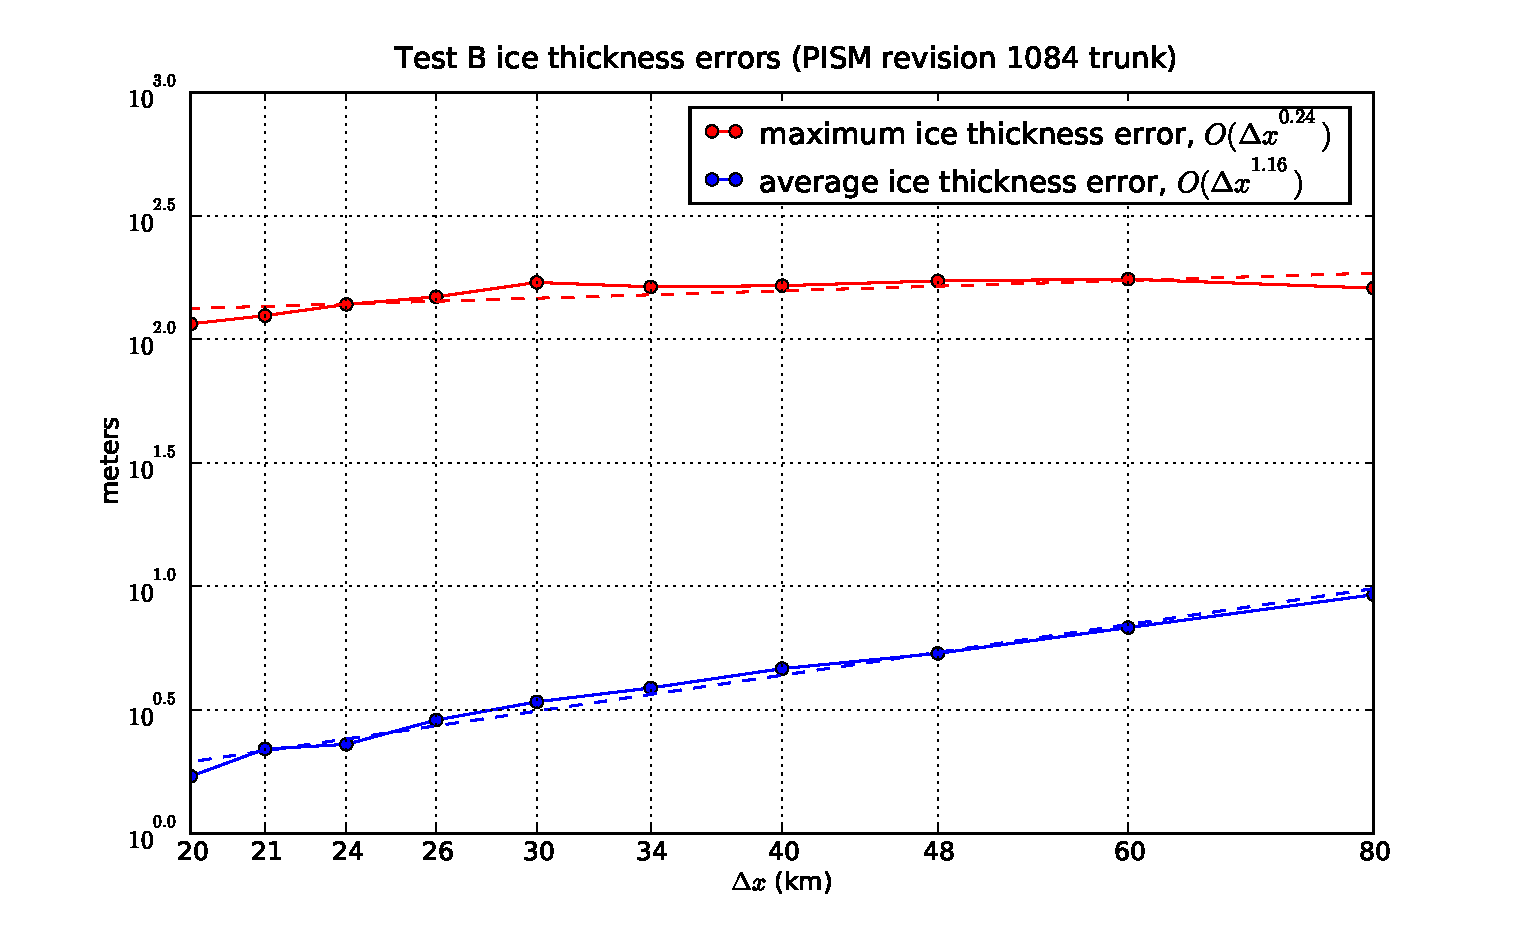
\includegraphics[width=4.8in,keepaspectratio=true]{test-B-thickness}
\caption{Numerical thickness errors in test B. See \cite{BLKCB} for discussion.}
\label{fig:thickerrsB}
\end{figure}

\begin{figure}[ht]
\centering
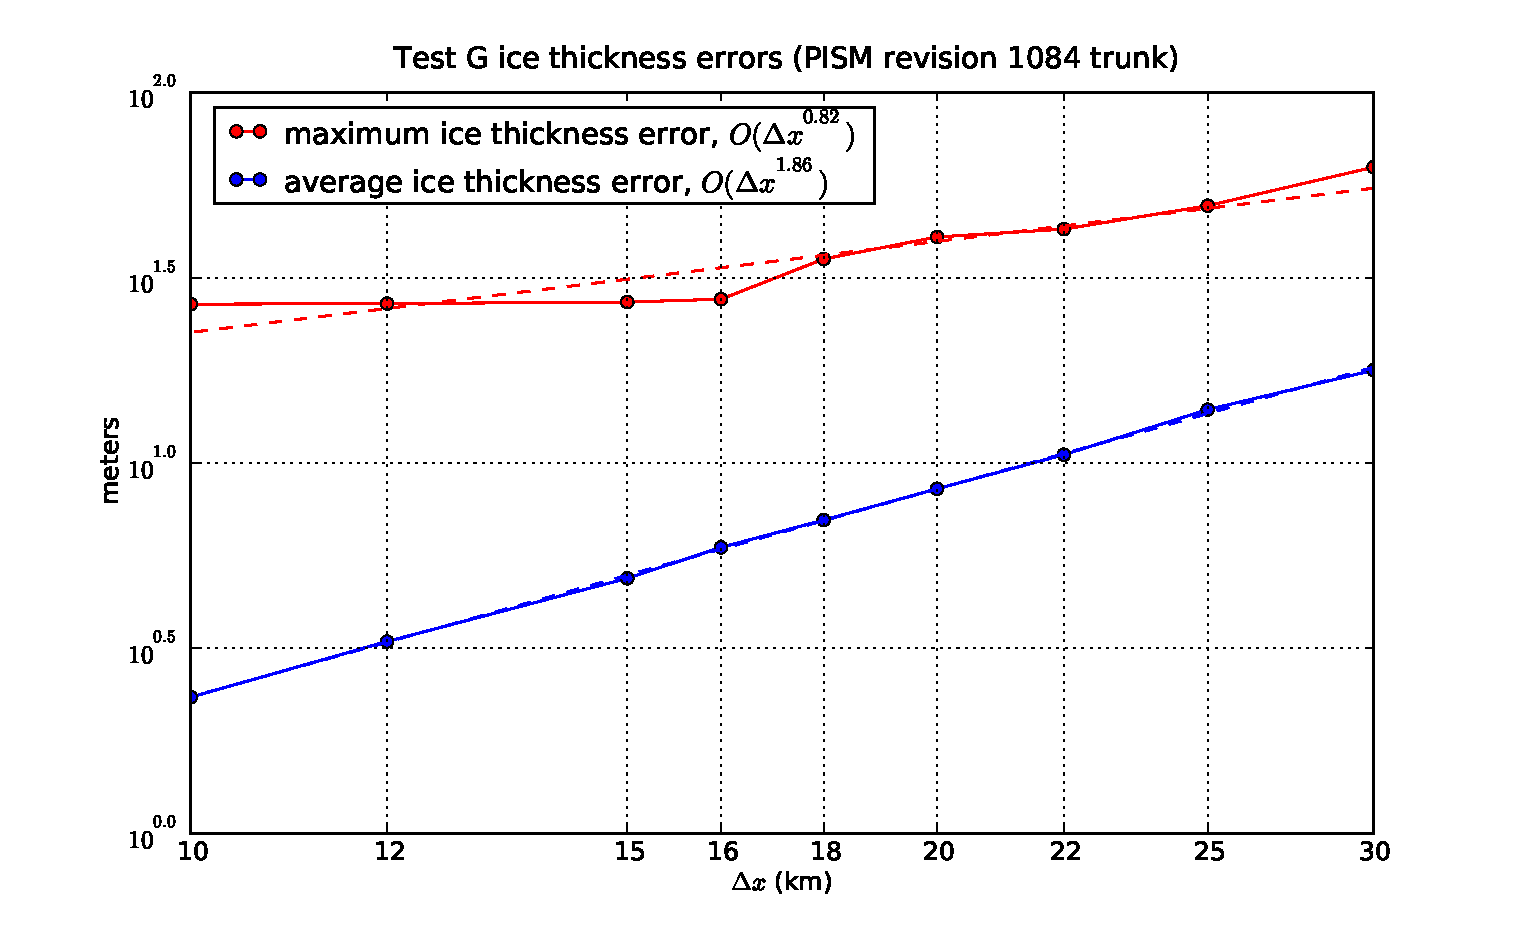
\includegraphics[width=5.0in,keepaspectratio=true]{test-G-thickness}
\caption{Numerical thickness errors in test G.  See \cite{BBL} and \cite{BLKCB}.}
\label{fig:thickerrsG}
\end{figure}

\begin{figure}[ht]
\centering
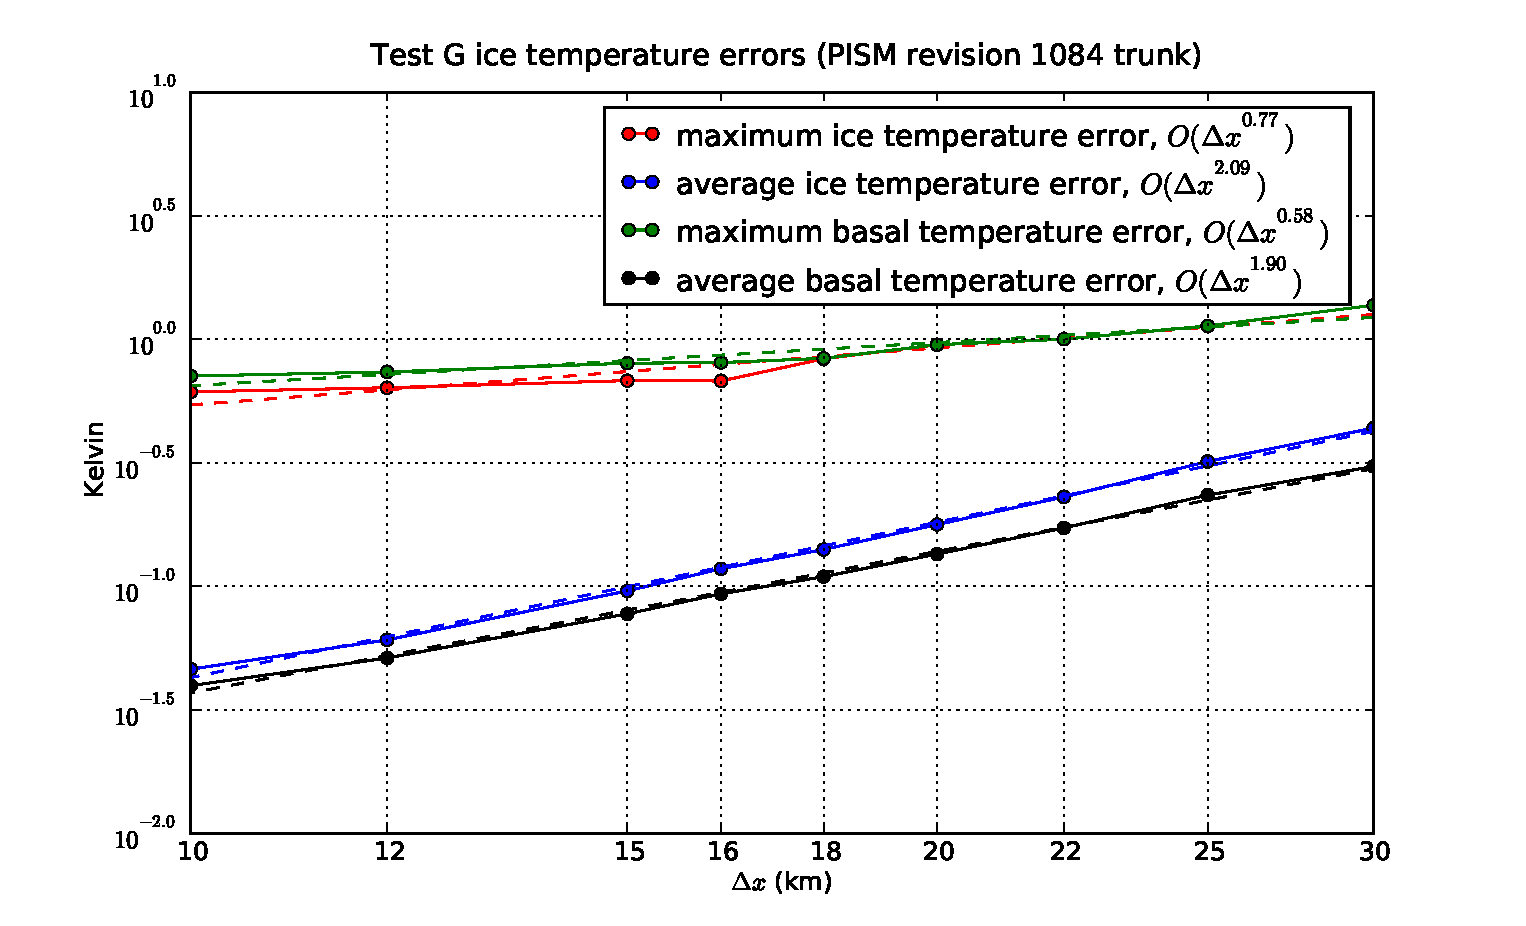
\includegraphics[width=5.0in,keepaspectratio=true]{test-G-temp}
\caption{Numerical temperature errors in test G. See \cite{BBL}.}
\label{fig:temperrsG}
\end{figure}

\begin{figure}[ht]
\centering
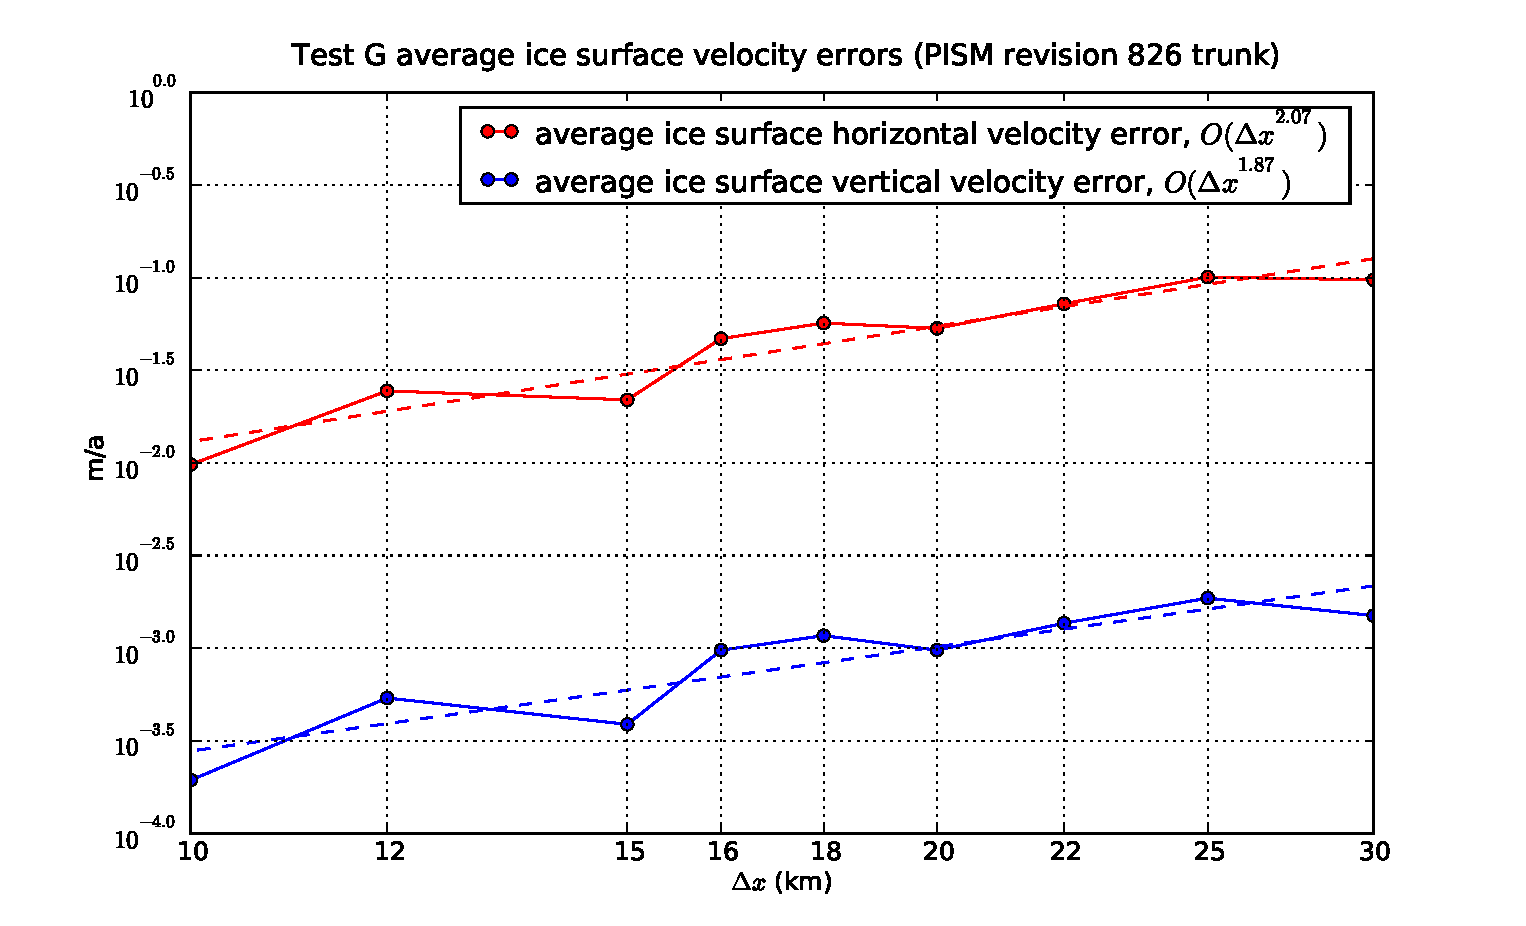
\includegraphics[width=5.0in,keepaspectratio=true]{test-G-surfvels}
\caption{Numerical errors in computed surface velocities in test G.}
\label{fig:surfvelerrsG}
\end{figure}

\begin{figure}[ht]
\centering
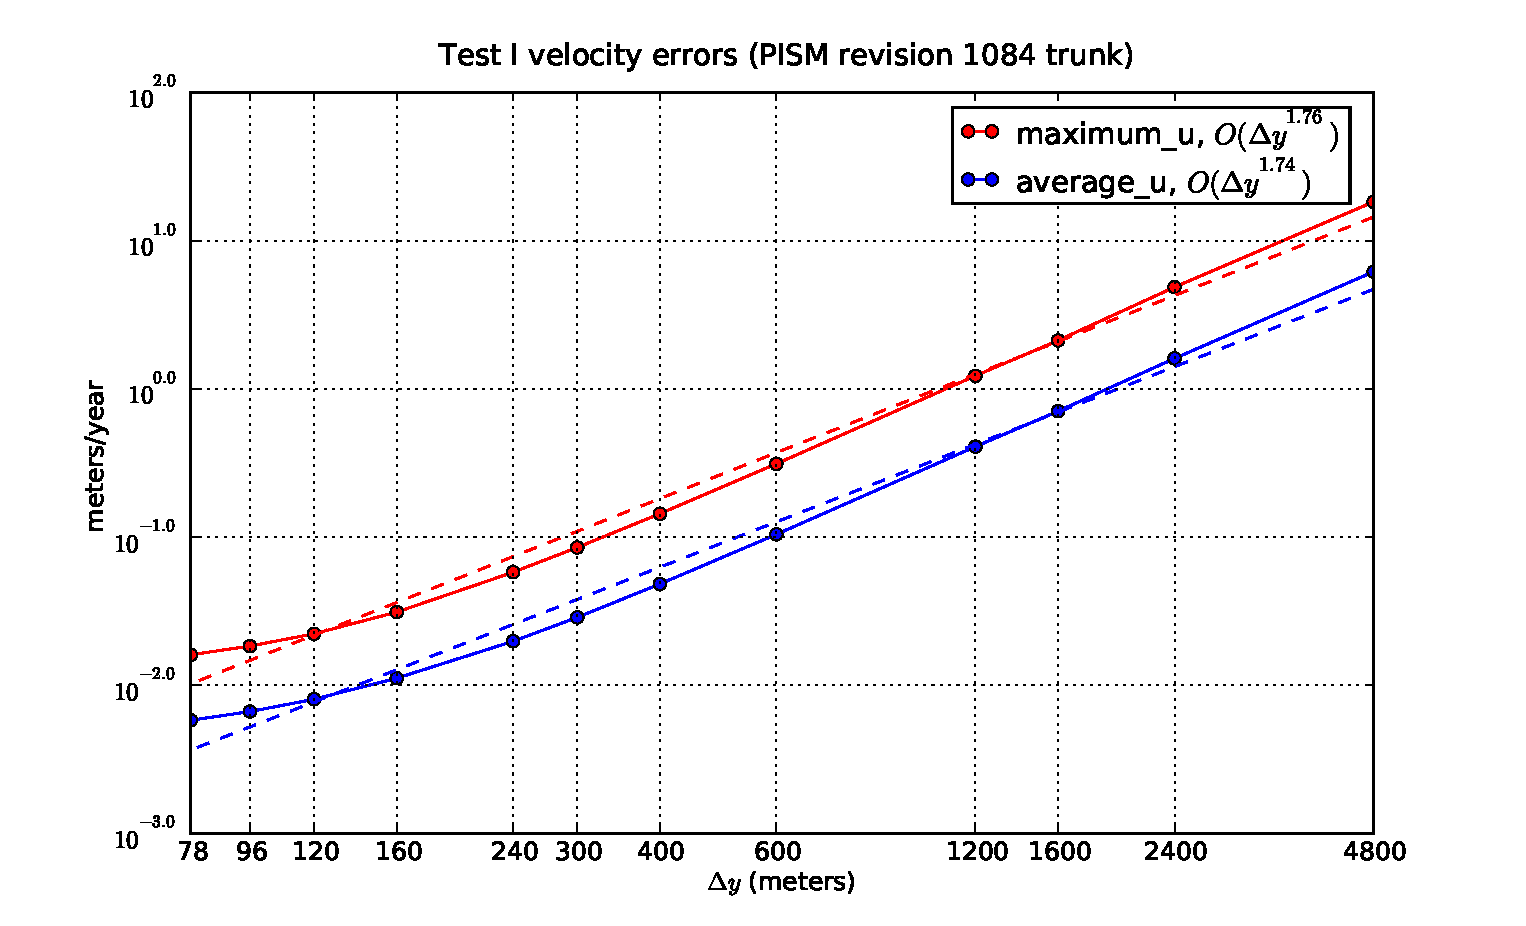
\includegraphics[width=5.0in,keepaspectratio=true]{test-I-errors}
\caption{Numerical errors in horizontal velocities in test I, an ice stream. \t{maximum_u} and \t{average_u} are errors in scalar velocity (because of symmetries in test I).  See \cite{SchoofStream,BBssasliding}.}
\label{fig:velerrsI}
\end{figure}

\begin{figure}[ht]
\centering
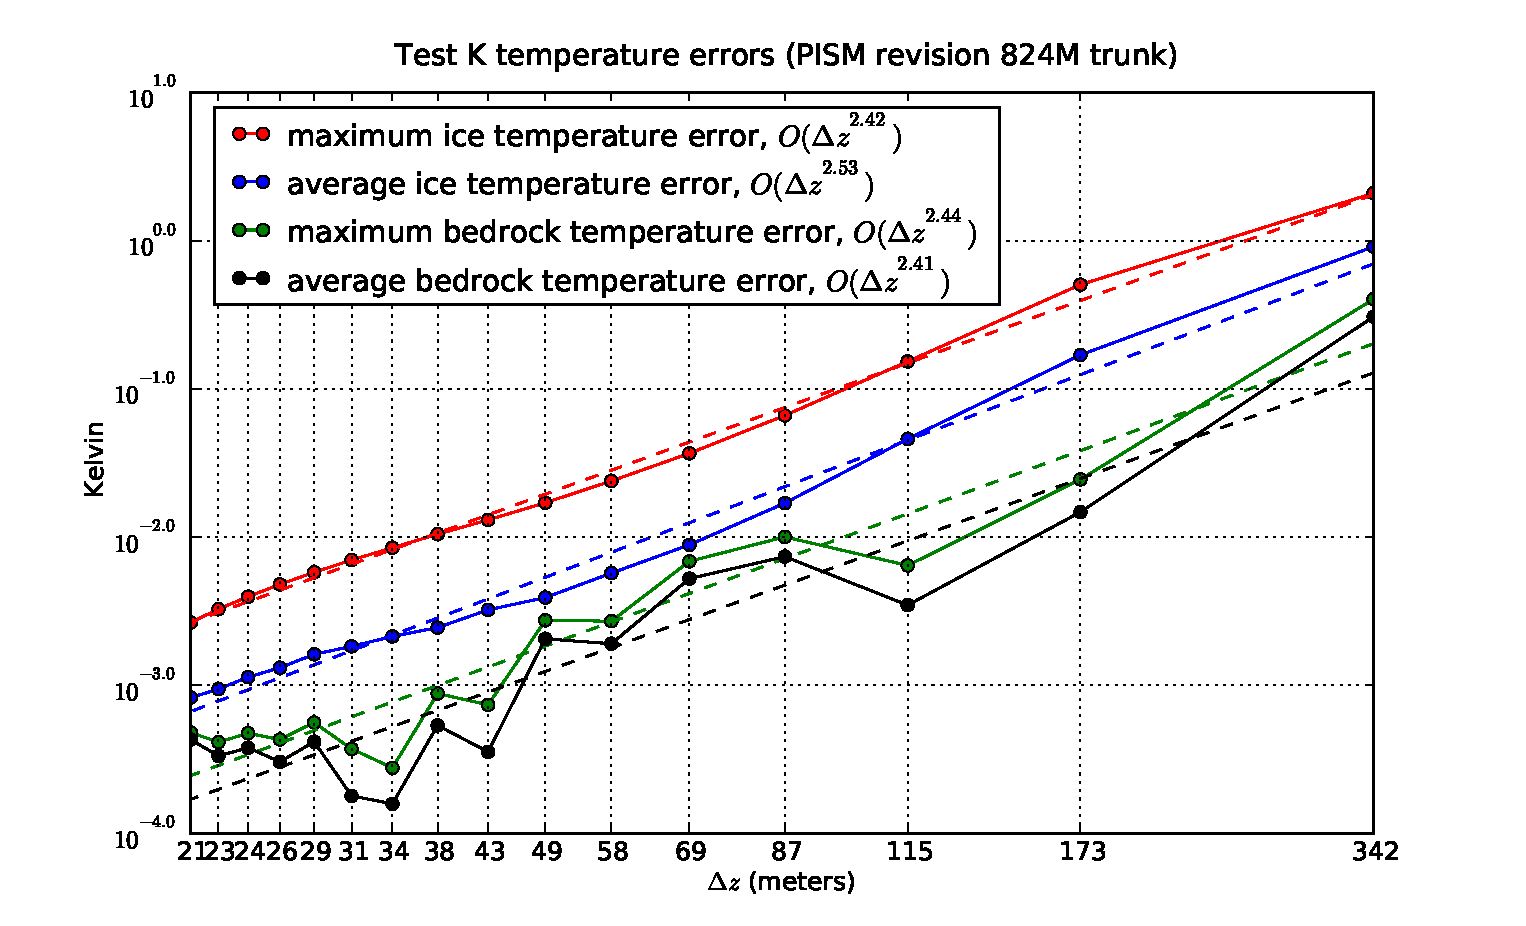
\includegraphics[width=5.0in,keepaspectratio=true]{test-K-errors}
\caption{Numerical temperature errors in test K, which tests the thermal bedrock model.  See \cite{BuelerTestK} for a discussion.}
\label{fig:temperrsK}
\end{figure}


%%% Local Variables: 
%%% mode: latex
%%% TeX-master: "manual"
%%% End: 


\clearpage\newpage

\section{Simplified geometry experiments with PISM}\label{sec:simp}

\subsubsection*{Historical note}  There have been three stages of ice sheet model intercomparisons based on simplified geometry experiments since the early 1990s \cite{BuelerSpray}.\index{EISMINT!defined}

EISMINT I \cite[ European Ice Sheet Modeling INiTiative]{EISMINT96}\footnote{See \url{http://homepages.vub.ac.be/\%7Ephuybrec/eismint.html}.} was the first of these and involved only the isothermal shallow ice approximation (SIA).  Both fixed margin and moving margin experiments were performed in EISMINT I, and various conclusions were drawn about the several numerical schemes used in the intercomparison.  EISMINT I is superceded, however, by verification using the full variety of known exact solutions to the isothermal SIA \cite{BLKCB}.  The ``rediscovery'', since EISMINT I, of the Halfar similarity solution with zero accumulation \cite{Halfar83}, and verification runs using that solution, already suffices to measure the isothermal SIA performance of PISM more precisely than would be allowed by comparison to EISMINT I results.

EISMINT II \cite{EISMINT00} pointed out interesting and surprising properties of the thermocoupled SIA.  References \cite{BBL,Hindmarsh04,Hindmarsh06,PayneBaldwin,SaitoEISMINT,BBssasliding} each interpret the EISMINT II experiments and/or describe attempts to add more complete physical models to ``fix'' the (perceived and real) shortfalls of ice sheet model behavior on EISMINT II experiments.  We believe that the discussion in \cite{PayneDongelmans,PayneBaldwin,BBL} adequately explains the ``spokes'' in EISMINT II experiment F as a genuine fluid instability, while Appendix B of \cite{BBssasliding} adequately cautions against the continuum model that generates the ``spokes'' in EISMINT II experiment H.   Thus we can move on from that era of controversy.  In any case, PISM has built-in support for all of the published and unpublished EISMINT II experiments; these are described in the next subsection.

The ISMIP (Ice Sheet Model Intercomparison Project)\footnote{See \url{http://homepages.vub.ac.be/\%7Ephuybrec/ismip.html}.}\index{ISMIP!defined} round of intercomparisons is still ongoing at this time (2009).  There are two components of ISMIP substantially completed, namely HOM = Higher Order Models \cite{ISMIPHOM,HOMelmer} and HEINO = Heinrich Event INtercOmparison \cite{GreveTakahamaCalov,Calovetal2009HEINOfinal}.  Of these, PISM participated in HEINO, but this ability is unmaintained.   We believe\index{ISMIP!interpretation of HEINO results} the continuum problem described by HEINO, also used in EISMINT II experiment H (above), is not easily approximate-able because of a required discontinuous jump in the basal velocity field.  The continuum problem predicts infinite vertical velocity because of this jump \cite[Appendix B]{BBssasliding}.  Details of the numerical schemes and their results are irrelevant if the continuum model makes such a prediction.

PISM offers the physical continuum model described in \cite{BBssasliding}, an SIA/SSA hybrid, as an alternative to the continuum model used in ISMIP-HEINO and EISMINT II experiment H.  Indeed the SIA/SSA hybrid is offered as a unified shallow model for real ice sheets (section \ref{sec:dynamics}).

There is no current plan to support ISMIP-HOM, but comparison of shallow PISM results to exact Stokes solutions is a goal for PISM evaluation.

A third ISMIP part is the Marine Ice Sheet Model Intercomparison Project (MISMIP and MISMIP3D)\index{ISMIP!MISMIP}.  It is minimally supported in PISM, as described in subsection \ref{subsect:MISMIP} and \ref{subsect:MISMIP3D} below.


\subsection{EISMINT II}\label{subsect:EISMINTII}
\optsection{EISMINT II}

There are seven experiments described in the published EISMINT II writeup \cite{EISMINT00}.\index{EISMINT}  They are named A, B, C, D, F, G, and H.  They have these common features:\begin{itemize}
\item runs are for 200,000 years, with no prescribed time step;
\item a $61\times 61$ horizontal grid on a square domain ($1500$ km side length) is prescribed;
\item the surface inputs (temperature and mass balance) have angular symmetry around the center of the grid;
\item the bed is flat and does not move (no isostasy);
\item the temperature in the bedrock is not modeled;
\item only the cold (not polythermal) thermomechanically-coupled shallow ice approximation is used \cite{EISMINT00}; and
\item though basal melt rates may be computed diagnostically, they do not affect the evolution of the ice sheet.
\end{itemize}
The experiments differ from each other in their various combinations of surface temperature and mass balance parameterizations.  Experiments H and G involve basal sliding, under the physically-dubious SIA sliding rubric \cite[Appendix B]{BBssasliding}, while the others don't.  Four experiments start with zero ice (A,F,G,H), while the other experiments (B,C,D) start from the final state of experiment A.

In addition to the seven experiments published in \cite{EISMINT00}, there were an additional five experiments described in the EISMINT II intercomparison description 
\cite{EISIIdescribe}, labeled E, I, J, K, and L.\index{EISMINT!unpublished additional EISMINT II experiments}  These experiments share most features listed above, but with the following differences.  Experiment E is the same as experiment A except that the peak of the accumulation, and also the low point of the surface temperature, are shifted by 100 km in both $x$ and $y$ directions; also experiment E starts with the final state of experiment A.  Experiments I and J are similar to experiment A but with non-flat ``trough'' bed topography.  Experiments K and L are similar to experiment C but with non-flat ``mound'' bed topography.

See table \ref{tab:eisII} for how to run all EISMINT II experiments in PISM.  Note that the vertical grid is not specified in EISMINT II, and it seems that good simulation of the thermomechanically-coupled conditions near the base of the ice requires relatively-fine resolution there.  (It is difficult to be quantitative because of a lack of theory.)  We suggest using the default unequally-spaced grid with 61 levels, which gives a grid spacing of 21 m in the ice layer closest to the bed.\footnote{An equally-spaced grid is an option in PISM, and in this case we suggest using 201 vertical levels to give 25 m spacing.}

These SIA-only simulations parallelize particularly well.  Very roughly, for the standard $61\times 61$ horizontal grid, wall-clock-time speedups will occur up to about 30 processors, and finer grids will benefit from even more processors, of course.

Table \ref{tab:eisII} shows how all EISMINT II experiments are done in PISM.  Experiments below the horizontal line in Table \ref{tab:eisII} are only documented in \cite{EISIIdescribe}.

\begin{table}[ht]
\centering
\small
\begin{tabular}{@{}llll}\toprule
\textbf{Command: ``\texttt{pisms }'' $+$} & \textbf{Relation to experiment A} \\
\midrule
\texttt{-eisII A -Mx 61 -My 61 -Mz 61 -y 200000 -o eisIIA.nc} & \\
\texttt{-eisII B -i eisIIA.nc -y 2e5 -o eisIIB.nc} & warmer \\
\texttt{-eisII C -i eisIIA.nc -y 2e5 -o eisIIC.nc} & less snow (lower accumulation)\\
\texttt{-eisII D -i eisIIA.nc -y 2e5 -o eisIID.nc} & smaller area of accumulation \\
\texttt{-eisII F -Mx 61 -My 61 -Mz 61 -y 2e5 -o eisIIF.nc} & colder; famous spokes \cite{BBL} \\
\texttt{-eisII G -Mx 61 -My 61 -Mz 201 -y 2e5 -o eisIIG.nc} & sliding (regardless of temperature) \\
\texttt{-eisII H -Mx 61 -My 61 -Mz 201 -y 2e5 -o eisIIH.nc} & melt-temperature activated sliding \\ \midrule
\texttt{-eisII E -i eisIIA.nc -y 2e5 -o eisIIE.nc} & shifted climate maps \\
\texttt{-eisII I -Mx 61 -My 61 -Mz 201 -y 2e5 -o eisIII.nc} & trough topography \\
\texttt{-eisII J -i eisIII.nc -y 2e5 -o eisIIJ.nc} & trough topography and less snow \\
\texttt{-eisII K -Mx 61 -My 61 -Mz 201 -y 2e5 -o eisIIK.nc} & mound topography \\
\texttt{-eisII L -i eisIIK.nc -y 2e5 -o eisIIL.nc} & mound topography and less snow \\
\bottomrule
\normalsize
\end{tabular}
\caption{Running the EISMINT II experiments in PISM.\index{PISM!running the EISMINT II experiments in}  Use \texttt{-skip -skip_max 5}, on the $61\times 61$ default grid, for significant speedup.}
\label{tab:eisII}
\end{table}

The EISMINT II experiments can be run with various modifications of the default settings.  Of course the grid can be refined.  For instance, a twice as fine grid in the horizontal is ``\texttt{-Mx 121 -My 121}''.  Table \ref{tab:eisIIoptions} lists some optional settings which are particular to the EISMINT II experiments.

\begin{table}[ht]
\centering
\small
\begin{tabular}{@{}lp{0.35\linewidth}lp{0.35\linewidth}}\toprule
\textbf{Option} & \textbf{Default values [expers]} & \textbf{Units} & \textbf{Meaning} \\\midrule
\intextoption{eisII} & A & &  Choose single character name of EISMINT II \cite{EISMINT00} simplified geometry experiment.  Allowed values are A, B, C, D, E, F, G, H. \\
\intextoption{Mmax} & 0.5 [ABDEFGHIK], 0.25 [CJL] & m$/$a & max value of accumulation rate \\
\intextoption{Rel} & 450 [ABEFGHIK], 425 [CDJL] & km & radial distance to equilibrium line \\
\intextoption{Sb} & $10^{-2}$ [\emph{all}] & (m/a)/km & radial gradient of accumulation rate \\
\intextoption{ST} & $1.67 \times 10^{-2}$ [\emph{all}] & K/km & radial gradient of surface temperature\\
\intextoption{Tmin} & 238.15 [ACDEGHIJKL], & K & max of surface temperature \\
 & 243.15[B], 223.15[F] & & \\
\intextoption{bmr_in_cont} & & & Include the basal melt rate in the mass continuity computation (override default for EISMINT II)\\
\bottomrule\normalsize
\end{tabular}
\caption{Changing the default settings for EISMINT II}
\label{tab:eisIIoptions}
\end{table}

In PISM the height of the computational box, the quantity set by \texttt{-Lz}, is set at the beginning of the run.  It is chosen for the EISMINT II experiments according to the observed maximum values occuring in standard runs.  If the ice thickens beyond the chosen level for the top of the computational box then additional layers are automatically added to the computational grid.  In fact, if the ice grows above the height of the computational box then a message appears, \texttt{PISM WARNING: max ice thickness ... is greater than the height of the computational box ...}, and then at least two additional levels are added to the vertical grid.  This is to some degree an emergency mechanism, however, because it can run away to use up all memory in extreme cases.  If the height of the computational box grows so large that the grid has more than twice the original number of vertical levels then PISM produces a \texttt{PISM ERROR} error message and stops.   Therefore it is possible that the number of vertical levels at the end of the run exceeds the initial \texttt{-Mz} value.  Setting EISMINT II options \texttt{-Mmax} or \texttt{-Sb} to produce higher accumulation rates than the default values (see table \ref{tab:eisIIoptions}) may cause the ice sheet to thicken above the standard thickness and therefore trigger this automatic extension mechanism.  Similarly, colder ice caused by nonstandard \texttt{-Tmin} or \texttt{-ST} values can produce unusually thick ice.  The user may always choose to use a larger, more conservative value for option \texttt{-Lz}, however.

See subdirectory \verb|examples/eismintII/| for a simple helper script \verb|runexp.sh|.


\subsection{MISMIP}\label{subsect:MISMIP}
\optsection{MISMIP}

This intercomparison addresses grounding line dynamics by considering an idealized one-dimensional stream-shelf system.  The intercomparison process is described at the website

\centerline{\url{http://homepages.ulb.ac.be/~fpattyn/mismip/}}

\noindent Find a full text description there.  It is essential reading for understanding MISMIP results generally, and for appreciating many of the comments in this subsection.

PISM's version of MISMIP includes an attached ice shelf even though modeling the shelf is theoretically unnecessary in the MISMIP flow line case.  The analysis in \cite{SchoofMarine1} shows that the only effect of an ice shelf, in the flow line case, is to transfer the force imbalance at the calving front directly to the ice column at the grounding line.  But this analysis does not apply to ice shelves with two horizontal dimensions, of course.  Real ice shelves have ``buttressing'' and ``side drag'' and other forces not present in flow line circumstances \cite{Goldbergetal2009}.  See the Ross ice shelf example in section \ref{sec:ross}, for example.

We use the usual PISM ice shelf model, with two horizontal dimensions, to do MISMIP.  This intercomparison therefore looks at the grounding line dynamics results from the usual PISM code, though in a highly symmetric case without side drag.

Because PISM is a model with two horizontal dimensions, we must adapt it to do a flow line problem (see section \ref{sec:flowline-modeling}). The flow direction for MISMIP is arbitrarily taken to be ``$x$''.  We periodize the cross-flow direction ``$y$'', and use the minimum number of points in this direction which maintains function.  This number turns out to be ``\texttt{-My 3}''; fewer points than this in the cross-flow direction confuses the finite difference scheme.

PISM has two applicable ice dynamics models. Model 1 is a pure SSA model.  It is ``category 2'' in the MISMIP classification.  Model 2 combines SIA and SSA velocities as described in \cite{BBssasliding}, and is ``category 3'' because it resolves ``vertical'' shear (i.e.~using SIA flow).

There are many runs for a complete MISMIP intercomparison submission.  There are $62$ runs for each model and grid choice, and there are two models and three (suggested) grid choices, so a full suite is $6 \times 62 = 372$ runs.  The finest grid runs account for all the compute time, however.  ``Grid mode 2'' in the MISMIP description is 1500 grid spaces in the flow line direction\footnote{This translates into 3001 grid \emph{points} in PISM's doubled computational domain.}, a very fine grid which imposes severe time-step restrictions on the explicit methods in PISM.  For the PISM MISMIP submission in Sept.~2008 we chose to only submit runs for a grid with 150 (``grid mode 1'') and 600 (``grid mode 3'') grid spaces in the flow line direction.  This was still 248 runs to submit, with 3 files each for a total of 744 text files.

Please see \texttt{README.md} in \texttt{examples/mismip/mismip2d} for a description of the setup that can be used to run MISMIP experiments in PISM.

\begin{figure}[ht]
\centering
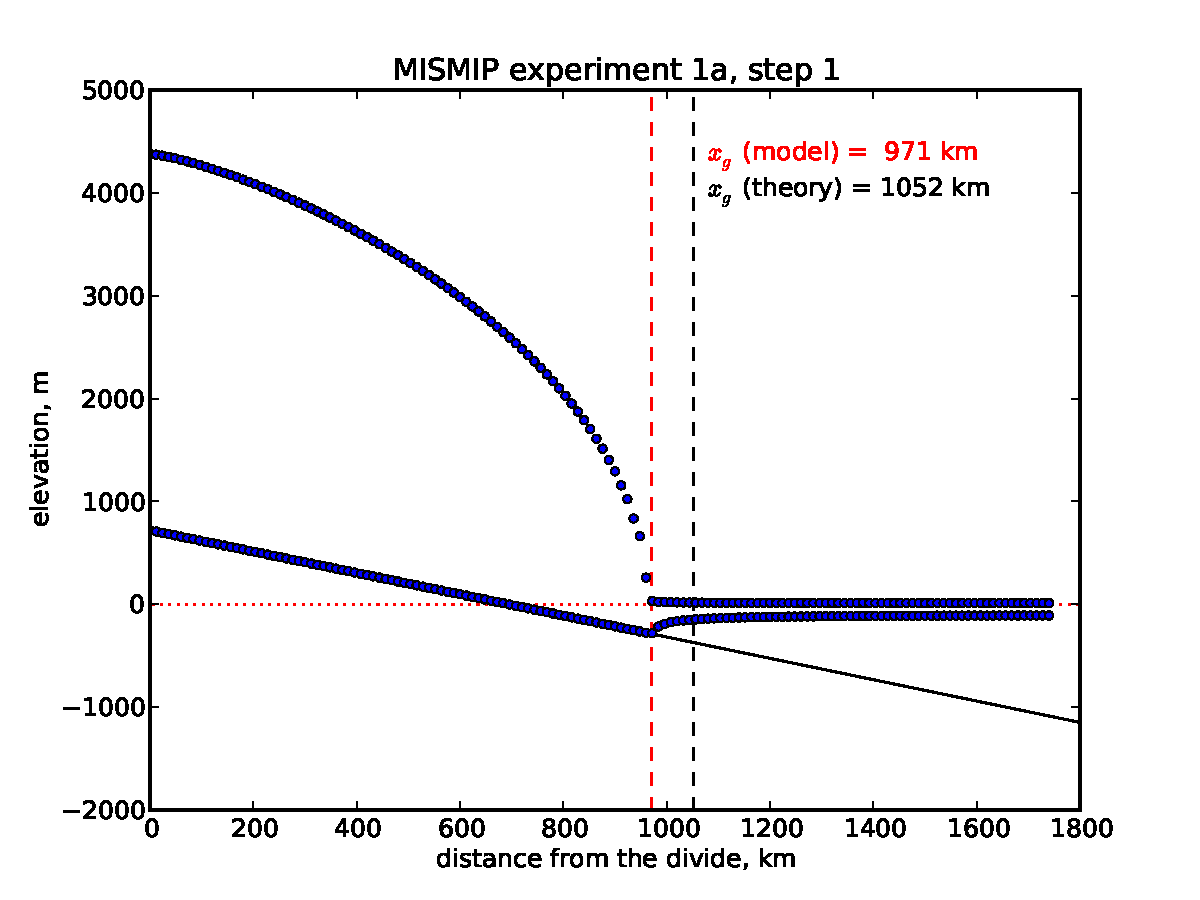
\includegraphics[width=4.0in,keepaspectratio=true]{CKH1-1a-M1-A1-profile}
\caption{A marine ice sheet profile in the MISMIP intercomparison; PISM model 1, experiment 1a, grid mode 1, step 1. Starting from a uniform $10$ m ice thickness.}
\label{fig:MISMIPmodel1exper1aM1A1}
\end{figure}

The implementation of MISMIP in PISM conforms fairly closely to the intercomparison description.  However, that document specifies
\begin{quotation}
\dots we require that the rate of change of grounding line position be $0.1$ m/a or less, while the rate of change of ice thickness at each grid point at which ice thickness is defined must be less than $10^{-4}$ m/a \dots
\end{quotation}
as a standard for ``steady state''. PISM does not include a stopping criterion such as ones described here. However, we report enough information, in PISM output files with scalar and spatially-variable time-series, to compute a grounding line rate or the time at which the thickness rate of change drops below $10^{-4}$ m/a.

One of the physical parameters regarding PISM's ice shelf model needs comment: we make the base of the ice shelves have very small resistance, using $10^{-4}$ times the linear drag typical of a Siple coast ice stream \cite{HulbeMacAyeal}, because this seems to have the effect of stabilizing the ice shelf.

\begin{figure}[ht]
\centering
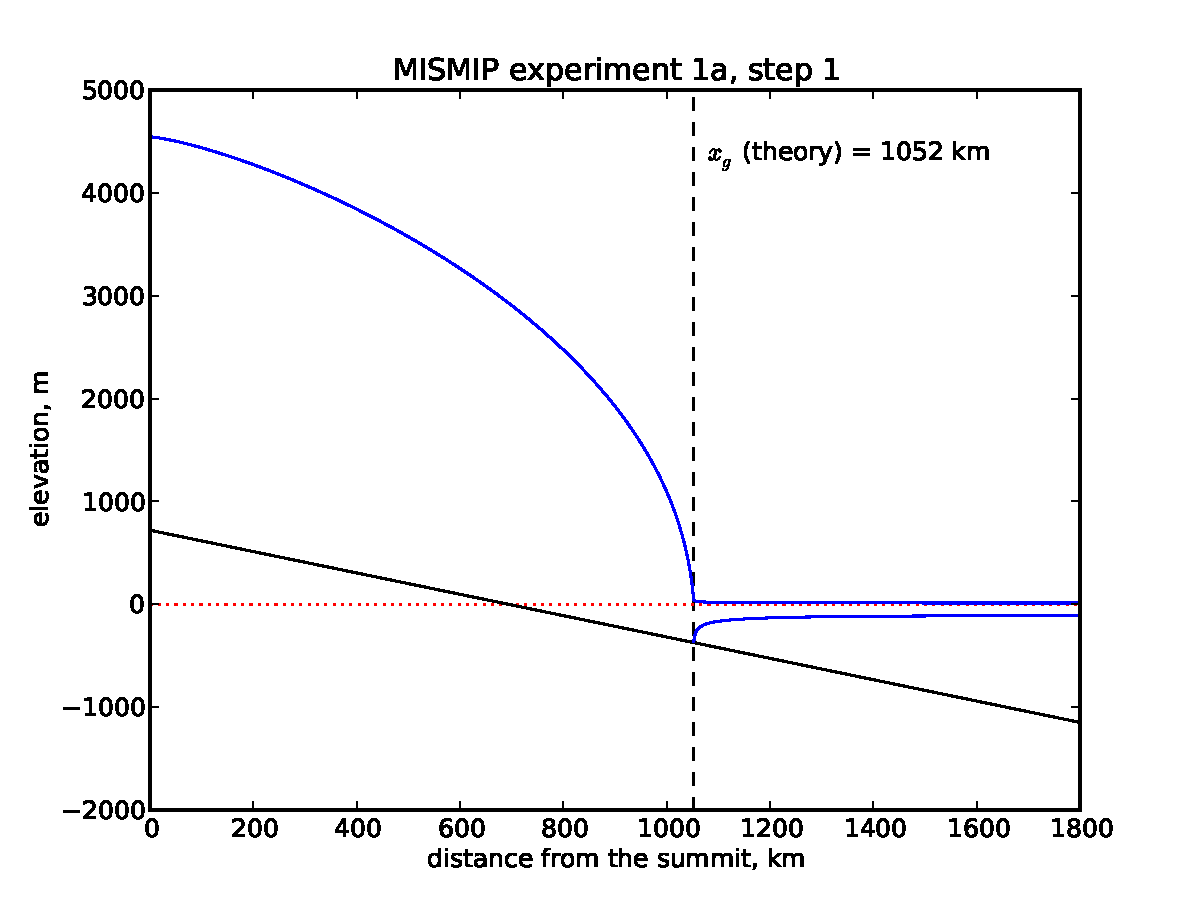
\includegraphics[width=4.0in,keepaspectratio=true]{SM-1a-A1}
\caption{Analytical profile for steady state of experiment 1a, grid mode 1, step 1, from theory in \cite{SchoofMarine1}.  This is a boundary layer asymptotic matching result, but not the exact solution to the equations solved numerically by PISM. Compare Figures \ref{fig:MISMIPmodel1exper1aM1A1} and \ref{fig:MISMIPmodel1exper1aM3A1FROMSM} generated by PISM.}
\label{fig:SMexper1aM1A1}
\end{figure}

The script \texttt{MISMIP.py} in \texttt{examples/mismip/mismip2d} has the ability to compute the profile from the Schoof's \cite{SchoofMarine1} asymptotic-matching boundary layer theory.  This script is a Python translation, using \texttt{scipy} and \texttt{pylab}, of the \Matlab codes in \url{http://homepages.ulb.ac.be/~fpattyn/mismip/MISMIP_distribution.tar}.  For example,

\begin{verbatim}
$ python MISMIP.py
\end{verbatim}

\noindent produces Figure \ref{fig:SMexper1aM1A1}.

We see immediately that the PISM result does not put the grounding line in the same location as Schoof's boundary layer theory.  We believe the problem is with PISM's numerical solution, not with that theory.  More evidence that the problem is numerical can be found by looking at the ice flux.  Using \texttt{ncview} to examine the diagnostic variable \texttt{cflx} (magnitude) in \texttt{ABC1_1a_M1_A1.nc} we see Figure \ref{fig:cflx1aM1A1}.  \emph{This is a problem with PISM}.  The flux should be a linear function.  Indeed, at steady state the flux $\bq$ solves $a=\Div\bq$ where $a$ is the accumulation rate.  In MISMIP, $a$ is the constant $0.3$ m/a, so at steady state $|\bq| = a x$, a line.

\begin{figure}[ht]
\centering
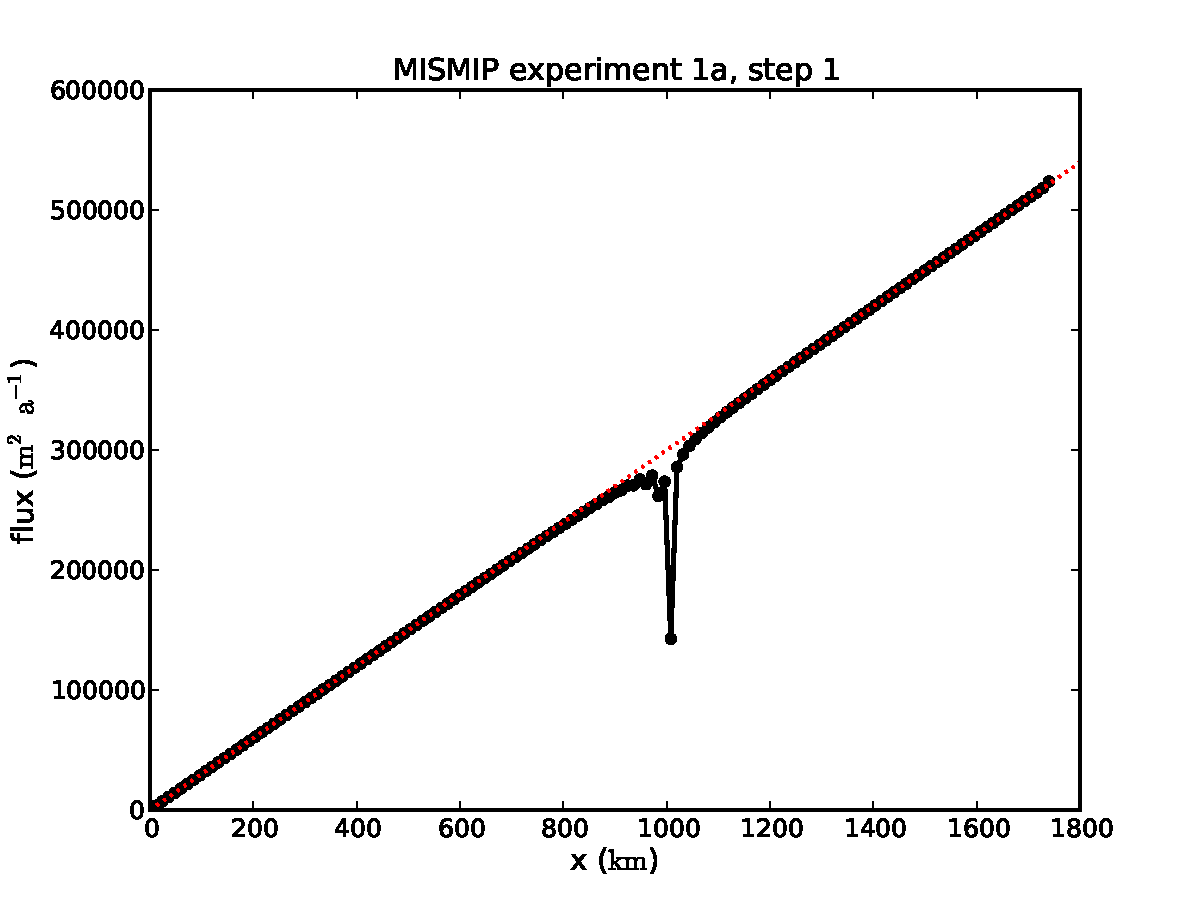
\includegraphics[width=4.0in,keepaspectratio=true]{CKH1-1a-M1-A1-flux}
\caption{Numerically computed flux $\bq = \bar\bU\, H$, where $\bar\bU$ is the vertically-averaged horizontal velocity and $H$ the thickness, for steady state of experiment 1a, grid mode 1, step 1.  Illustrates a significant numerical problem; it should be the dotted line, which has slope $a = 0.3$ m/a.}
\label{fig:cflx1aM1A1}
\end{figure}

We can learn more about the problem.  It turns out that the numerical flaw in the flux also keeps the grounding line from moving properly, we think.  The problem is that the numerical result doesn't move the grounding line to its correct location if the ice sheet and shelf are initially $10$ m as specified in MISMIP.  On the other hand, the correct location for the grounding line is also approximately a steady state for PISM numerics; the grounding line stays where you put it (compare \cite{SchoofMarine2} and \cite{VieliPayne}).

In fact, by default \texttt{run.py} uses the asymptotic-matching thickness result from the \cite{SchoofMarine1} theory to initialize the initial ice thickness, as allowed by the MISMIP specification.

The effect when we do this at higher resolution (grid mode 3 with 6km spacing, instead of 24 km), is a step forward.
The result, Figure \ref{fig:MISMIPmodel1exper1aM3A1FROMSM}, is more satisfactory.  On the other hand, inspection of the flux for this new run shows a smaller, but similarly worrying, jump in flux.

\begin{figure}[ht]
\centering
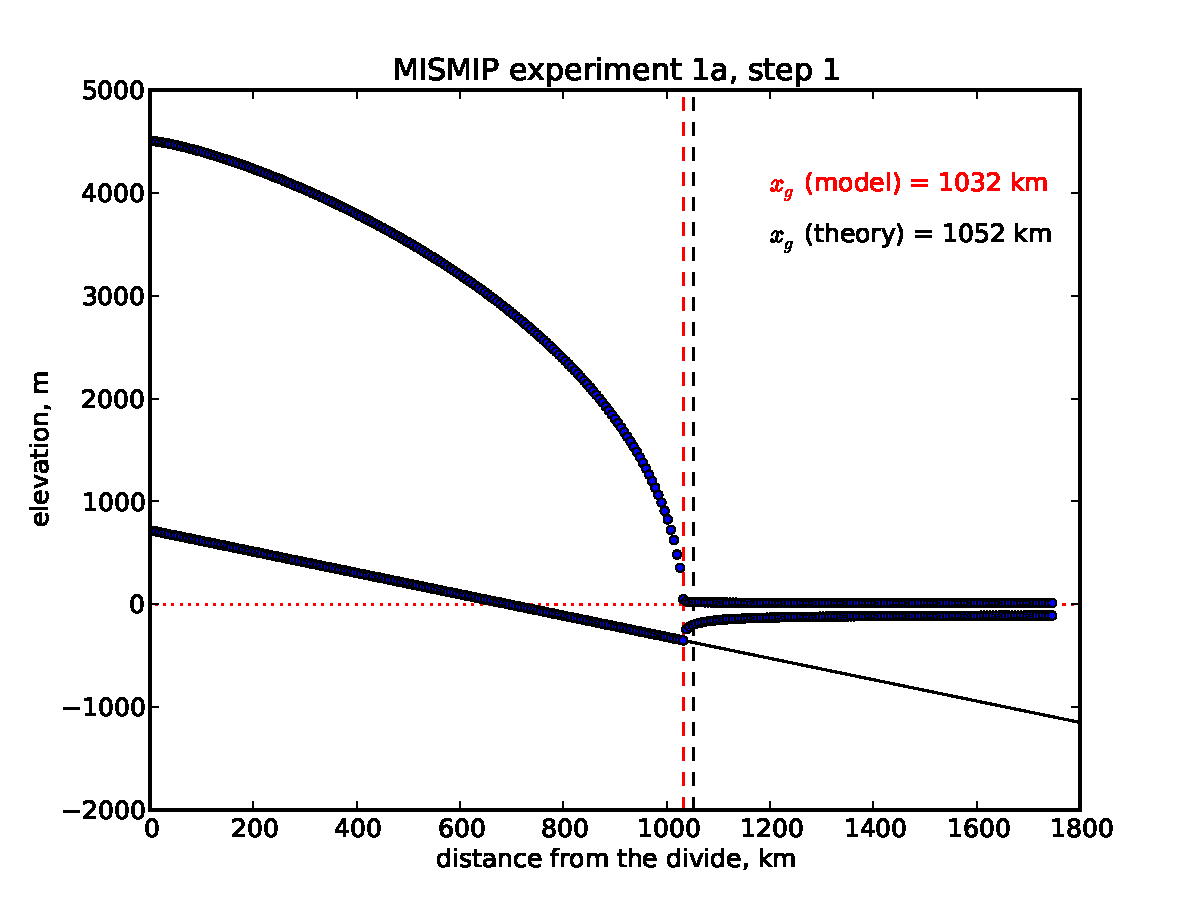
\includegraphics[width=4.0in,keepaspectratio=true]{CKH1-1a-M3-A1-profile}
\caption{A marine ice sheet profile in the MISMIP intercomparison; PISM model 1, experiment 1a, grid mode 3, step 1, but on a run started from the corresponding asymptotic-matching result.  At least the location of the grounding line agrees more closely with that in Figure \ref{fig:SMexper1aM1A1}.}
\label{fig:MISMIPmodel1exper1aM3A1FROMSM}
\end{figure}



\subsection{MISMIP3D}\label{subsect:MISMIP3D}
\optsection{MISMIP3D}

 The ice2sea MISMIP3D Marine Ice Sheet Model Intercomparison Project is a two-dimensional expansion of the MISMIP experiments for the flowline case as described above. The initial MISMIP3D setup is very close to MISMIP and considers ice flow in one direction. As in MISMIP, the grounding line position and its reversibility under changes of physical parameters is analyzed. However, in MISMIP3D not the ice softness $A$ is varied but the basal friction $\tau_C$ and the applied perturbation of the basal friction is punctual so that a curved grounding line is obtained. In contrast to the MISMIP experiments, no (semi-)analytical solutions are available to compare the numerical results against. A full description of the intent of the MISMIP3D experiments analogous to MISMIP can be found at

\centerline{\url{http://homepages.ulb.ac.be/~fpattyn/mismip3d/}}

 A complete set of MISMIP3D experiments consists of three runs: Firstly, an one-dimensional ice shield on a linearly sloped bed, similar to the MISMIP experiments, is run into a steady state (``standard experiment''). For this symmetrical stream-shelf geometry then a punctual sliding perturbation is applied, leading to a curved grounding line (``perturbation experiment'') after a fixed experiment-runtime of $100$ years. As a third step, beginning from the final state of the perturbation experiment, the sliding perturbation is removed and the system is run again into a steady state (``reversibility experiment''). Corresponding to the results of \cite{SchoofMarine1}, stating that a particular ice geometry only depends of its stationary physical parameters and boundary conditions and not of how it is dynamically reached, the resulting geometry of the reversibility experiment, in particular the grounding line position, should be identical to the result of the standard experiment.

For the execution of MISMIP3D experiments with PISM a Python script for generating a shell script template with all commands and options for running a complete set of MISMIP3D experiments is stored in the examples folder in \texttt{examples/mismip/mismip3d}. Also, a \texttt{README.md} file with all information of how to generate the shell script can be found in that folder.

For the flowline-case standard experiment, as in the MISMIP case, a computational domain with three grid points in the direction orthogonal to the ice flow (arbitrarily chosen as y-direction) is chosen in the template. For the perturbation and reversibility experiments a domain is defined which is symmetric along the ice-divide (mirror symmetry) and along the center line of the ice flow, while the side boundaries are periodic, which corresponds to a free-slip condition for the flow in x-direction. Though this choice of the symmetric computational domain increases computational cost, it allows to use standard PISM without fixing certain boundary conditions in the code.

PISM participated in the MISMIP3D intercomparison project with version Stable 0.5. The results are published in \cite{MISMIP3D2012} and can be reproduced by exactly using the mentioned shell script (with code version Stable 0.5). For PISM, $8=2^3$ different sets of results had been submitted for that publication: with and without SIA-computation, with and without subgrid linear grounding line interpolation (LI in \cite{Gladstoneetal2012}) and for two different resolutions (16.6 km and 1 km). For the standard experiment, we chose a computation time of $30000$ years (compare the comments to PISM's missing stopping criterion in the previous chapter). Because of the large computing time, for the reversibility experiment, we accepted a thickness rate of change smaller than $10^{−2}$ m/a as a criterion for having reached a steady state. This rate was reached after a fixed computation time of $500$ years in all cases. Furthermore, as demanded in the MISMIP3D experiment instructions, the grounding line reached a static position after that time.

We observed a considerable improvement of the results with respect to the absolute grounding line positions compared to other models (e.g. the FE reference model Elmer/Ice) and to the reversibility when applying the subgrid grounding line interpolation method\footnote{The subgrid groundling line interpolation method is available from PISM version v0.5-5-g7f98e2b (commit db132adf671e6cc769f90af8b5577edd6bb04ade on 5/30/12).} (See Figs.~\ref{fig:Subgl}). Furthermore, we observed that only using SSA yields almost the same results as the full hybrid SIA+SSA computation for the MISMIP3D (and also the MISMIP) experiments, but -- by not applying the SIA computation -- after a considerably shorter computation time (about 10 times shorter). We explain the small and almost negligible SIA velocities for the MISMIP(3D) experiments with the comparably small ice surface gradients in the MISMIP(3D) ice geometries. See Fig.~\ref{fig:compSIASSA} for a comparison of SSA and SIA velocities in the MISMIP3D geometry.

\begin{figure}[ht]
\centering
%\subfigure{
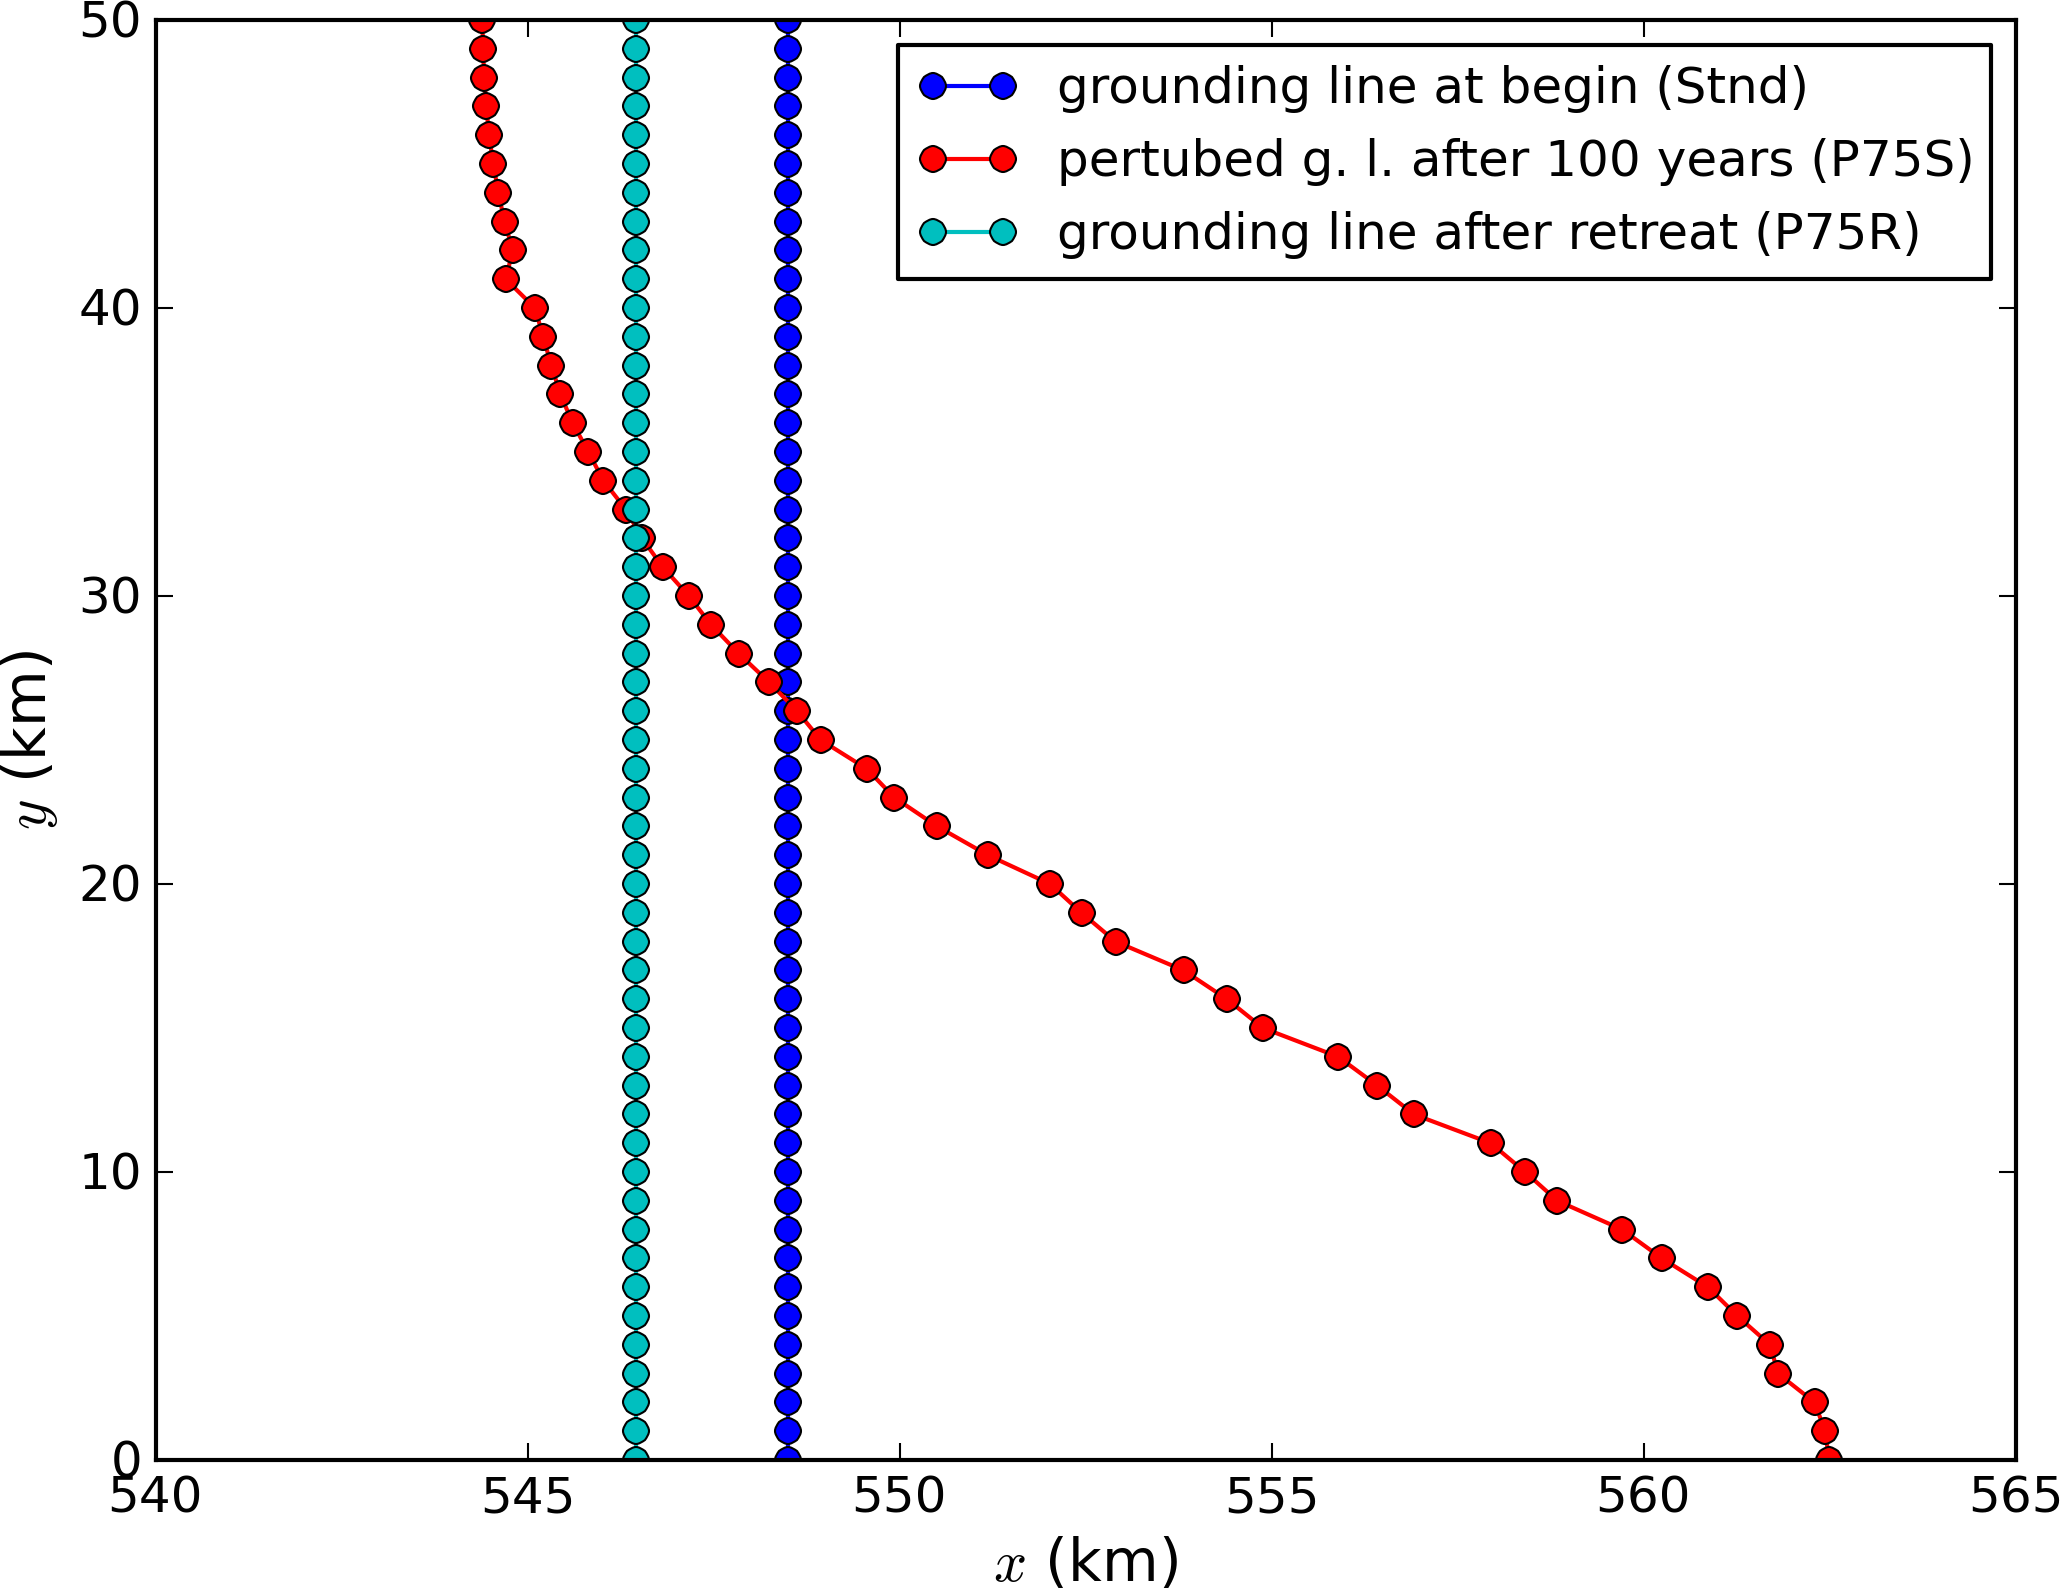
\includegraphics[width=3.0in,keepaspectratio=true]{Subgl}
%}
%\subfigure{
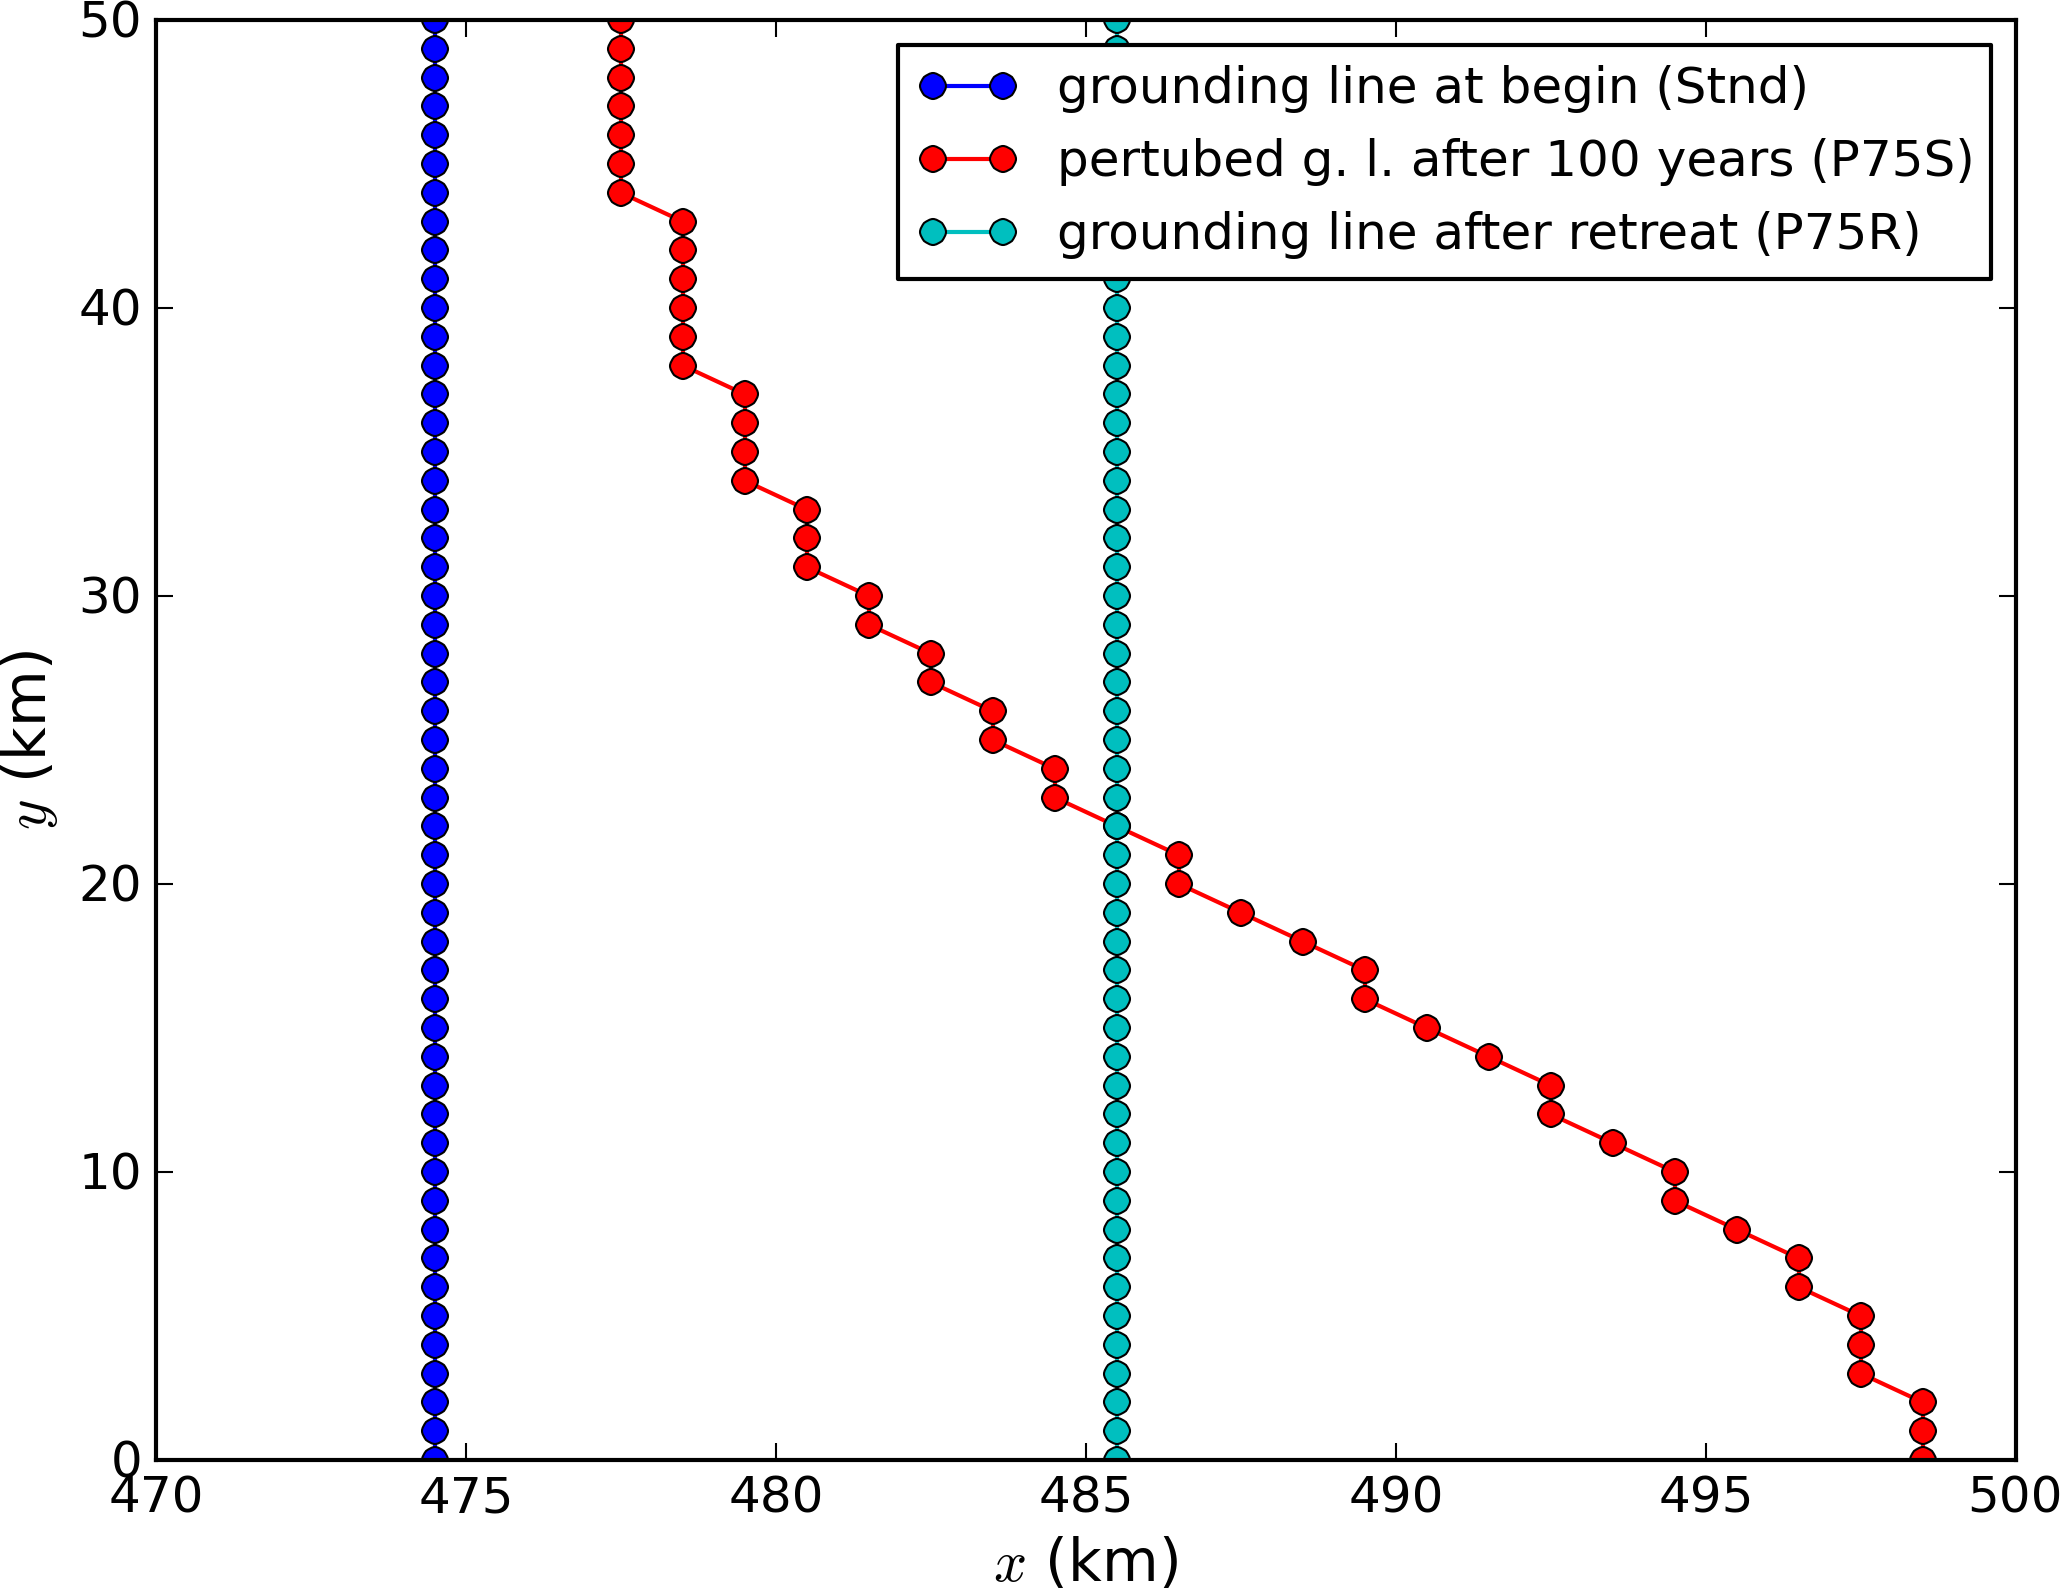
\includegraphics[width=3.0in,keepaspectratio=true]{NoSubgl}
%}
\caption{Comparision between the resulting grounding lines of the MISMIP3D experiments performed with PISM when using the subgrid grounding line interpolation method (a) and without (b). In both cases the SIA+SSA hybrid is used for a resolution of $\Delta x = \Delta y = 1\;$km (accumulation rate $0.5\;$m/a).}
\label{fig:Subgl}
\end{figure}

\begin{figure}[ht]
\centering
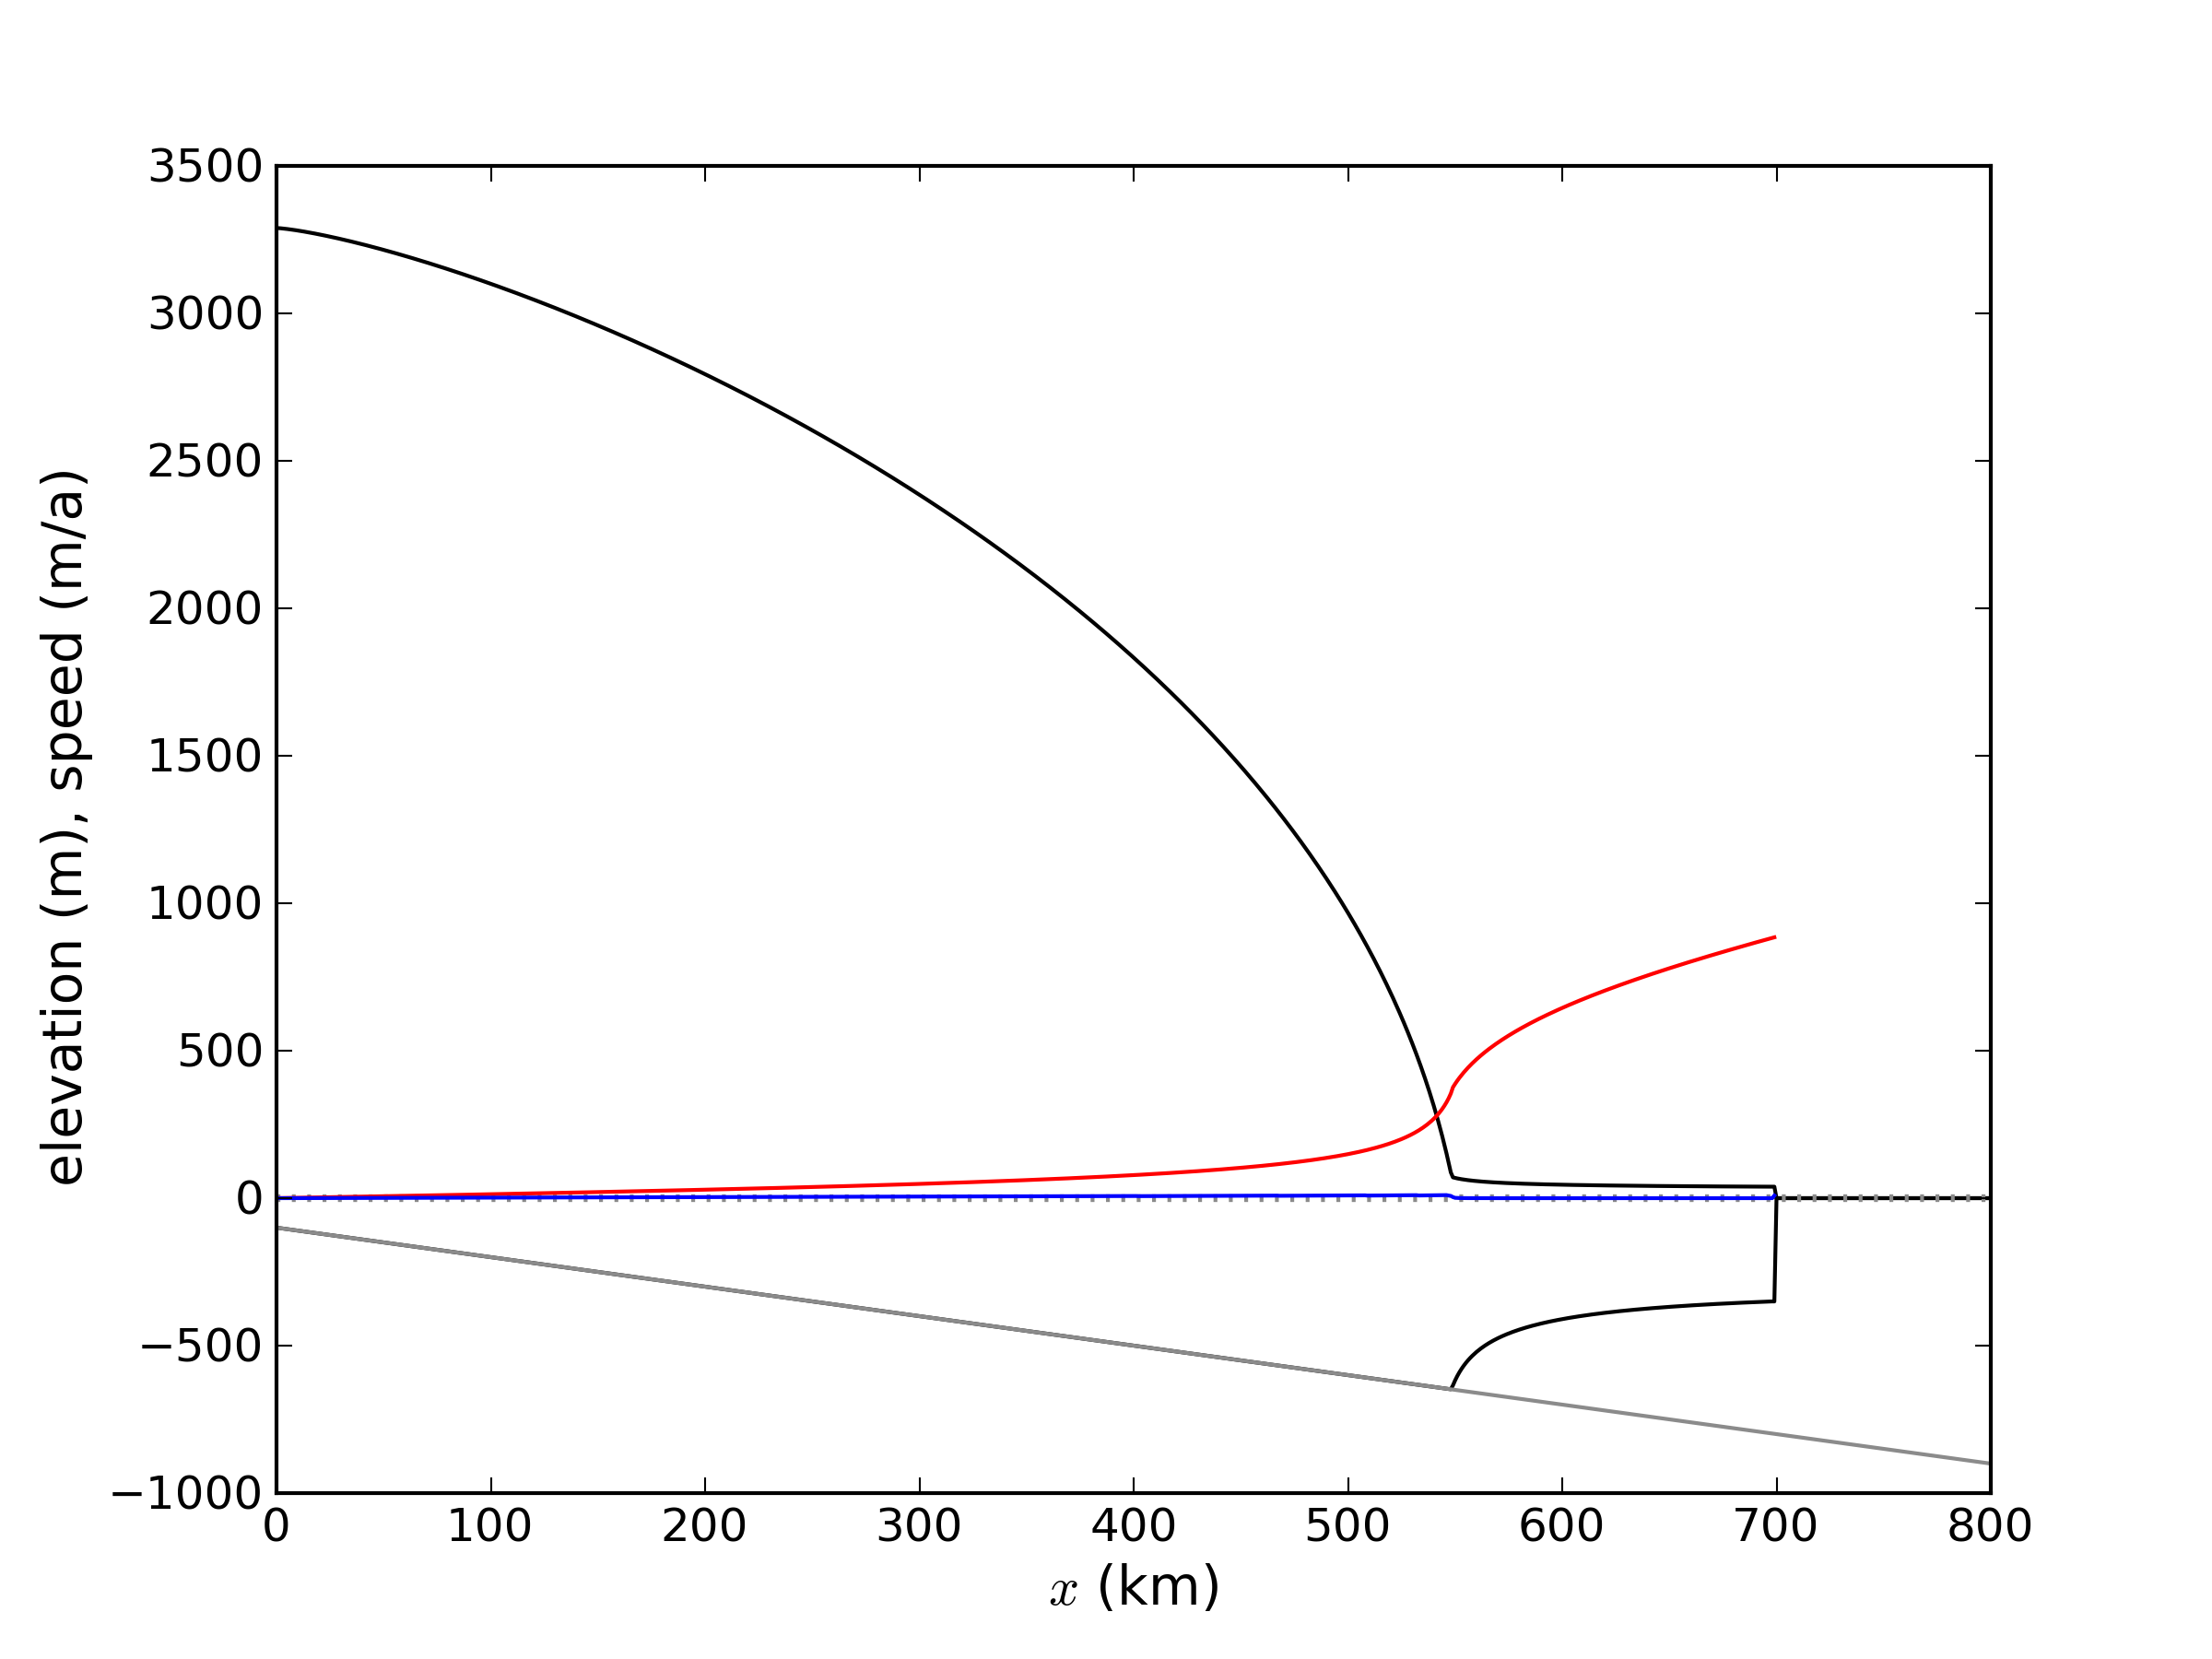
\includegraphics[width=5.0in,keepaspectratio=true]{comp-SIA-SSA}
\caption{Illustration of the negligible SIA velocities for the MISMIP3D standard experiment. The steady state ice geometry (accumulation rate $0.5\;$m/a, numerical resolution $\Delta x = 1\,$km) is plotted (black) together with the computed SSA velocity (red) and SIA velocity (blue). The SIA velocity is very smalland reaches its maximum value at the grounding line with about $10\,$m/a.}
\label{fig:compSIASSA}
\end{figure}

%%% Local Variables: 
%%% mode: latex
%%% TeX-master: "manual"
%%% End: 


\clearpage\newpage

\section{Example: Modeling the Greenland ice sheet (EISMINT-Greenland)}\label{sec:eismint-greenland} \index{PISM!running the EISMINT-Greenland intercomparison}\index{Ice Sheets!Greenland ice sheet}\index{EISMINT!intercomparison of Greenland models} 
\optsection{EISMINT-Greenland}

In this section we give an extended example of how to use PISM to model the Greenland ice sheet.  We use older data from the 1990s ice sheet modelling intercomparison EISMINT-Greenland \cite{HuybrechtsEISMINT,RitzEISMINT}, but it is an excellent tutorial example.

The data are freely available at

\begin{center}
  \url{http://homepages.vub.ac.be/~phuybrec/eismint/greenland.html}
\end{center}

\noindent The snow-fall accumulation map, ablation parameterization, surface temperature formula, surface elevation, and bedrock elevation maps are essentially as in the 1991 papers \cite{Letreguillyetal1991,OhmuraReeh}.  In the ``forced climate'' CCL3 run, described below, the modeled ice sheet is sees changes in surface temperature from the GRIP core \cite{Dansgaardetal1993} and sea level changes from SPECMAP \cite{Imbrieetal1984}.

Substantial developments have occurred in modeling the Greenland ice sheet since the EISMINT-Greenland intercomparison.  For example, the relation between a Greenland ice sheet flow model, Earth deformation under ice sheet loads, and the reconstruction of global ice loading is analyzed in \cite{TarasovPeltier}.  A parameter-sensitivity study of a EISMINT-Greenland-type ice sheet model is described in \cite{RitzFabreLetreguilly}.  The response of Greenland ice sheet models to climate warming is addressed in \cite{HuybrechtsdeWolde,Huybrechts02, Greve00}, among other references.

The rest of this section is a step-by-step PISM tutorial.  The details can be typed in by hand, or the user can invoke the bash scripts \texttt{preprocess.sh}, \texttt{bootstrap.sh}, \texttt{ssl2.sh}, and \texttt{ccl3.sh} in the directory \texttt{examples/eisgreen}.  These scripts execute the commands in the next four subsections, respectively.

\subsubsection*{Obtaining and pre-processing the EISMINT-Greenland data}  We use two Python scripts to convert the EISMINT-Greenland data.  The data is in the form of several ASCII text files, so we convert them into NetCDF files usable by PISM.  The Python libraries \href{http://numpy.scipy.org/}{\texttt{numpy}} and \href{http://code.google.com/p/netcdf4-python/}{\texttt{netcdf4-python}} must be present for the scripts to work.

First, \texttt{cd examples/eisgreen/} from the PISM directory, and download these text (ASCII) files from the EISMINT-Greenland web site above: 

\begin{verbatim}
grid20-EISMINT,  suaq20-EISMINT,  specmap.017,  sum89-92-ss09-50yr.stp
\end{verbatim}

\noindent (This is done by \texttt{preprocess.sh} using \texttt{wget}.) Once all four files have been downloaded, run

\begin{verbatim}
$ ./eisgreen.py
\end{verbatim}%$

\noindent The NetCDF file \texttt{eis_green20.nc} will be created from the data in \texttt{grid20-EISMINT} and \texttt{suaq20-EISMINT}.  It contains variables for the gridded latitude (\texttt{lat}), longitude (\texttt{lon}), surface altitude (``\texttt{usurf}'' for \textbf{u}pper \textbf{surf}ace elevation), ice thickness (\texttt{thk}), bedrock altitude (\texttt{topg}), and snow precipitation rate (\texttt{snowprecip}; in ice-equivalent thickness units).  These values can be viewed graphically with \texttt{ncview}.  The metadata for these variables (the NetCDF ``header'') can be viewed by

\begin{verbatim}
ncdump -h eis_green20.nc
\end{verbatim}

The bed elevation \texttt{topg} in the original data (\texttt{suaq20-EISMINT}) effectively contains missing values.  These are locations where \texttt{topg} is \emph{exactly} $0.0$, presumably because in these locations the observed bed elevation was not measured or the measured value was not trusted.  We think these are deep fjords locations, mostly.  Also the topography of Ellesmere island is replaced by out of range negative values.  When viewing \texttt{eis_green20.nc} with \texttt{ncview}, these values show as white spots.  

If these missing values were to be left in the NetCDF handed to PISM then the resulting (very) rough bed elevation map would make reasonable ice flow results difficult.  We therefore smoothly fill the holes in the bed elevations.  This is done with another script named \texttt{fill_missing.py}\index{executables!python scripts!\texttt{fill_missing.py}}:\footnote{\texttt{fill_missing.py} is a general tool for smoothly filling patches of missing values in variables in NetCDF files.  It looks for attributes defining missing values and then fills in specified variables essentially by averaging the neighboring non-missing values.  It is found in directory \texttt{pism/util/}, it requires \href{http://code.google.com/p/netcdf4-python/}{\texttt{netcdf4-python}}, and it is documented in subsection \ref{subsect:scripts}.}:

\begin{verbatim}
$ fill_missing.py -f eis_green20.nc -v topg -o eis_green_smoothed.nc
\end{verbatim}%$

\begin{figure}[ht]
\centering
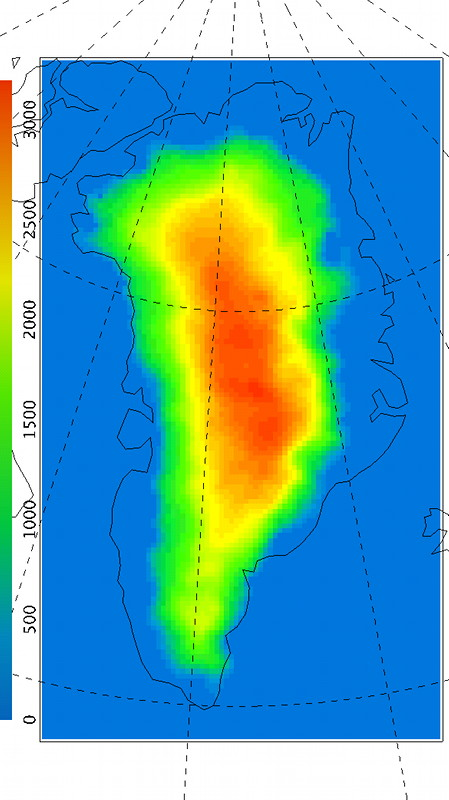
\includegraphics[width=2.4in,keepaspectratio=true]{EISgreen-thick}\quad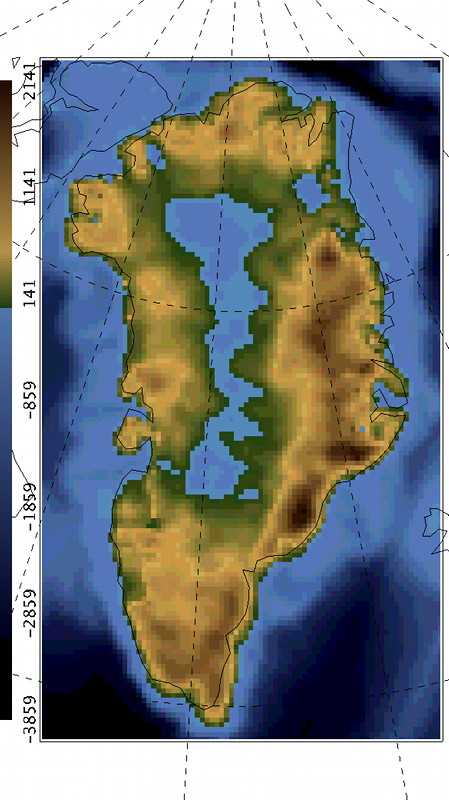
\includegraphics[width=2.4in,keepaspectratio=true]{EISgreen-bed}
\caption{Views of the thickness (left) and smoothed bed elevation (right) for EISMINT-Greenland.  The coastal topography around several fjords has been smoothed.}
\label{fig:greendata}
\end{figure}

Next we use a script which converts the time-series data files \texttt{specmap.017} and \texttt{sum89-92-ss09-50yr.stp} to PISM-readable NetCDF form:

\begin{verbatim}
$ ./eiscore.py
\end{verbatim}%$

\noindent Two NetCDF files with one-dimensional time series data are created, namely \texttt{grip_dT.nc} and \texttt{specmap_dSL.nc}.  In the paleoclimate run ``CCL3'' below, the executable \texttt{pgrn} will be called with options \texttt{-dTforcing} and \texttt{-dSLforcing} on these two \texttt{.nc} files, respectively.  Thus PISM will read the GRIP data \cite{Dansgaardetal1993} for the surface temperature forcing and the SPECMAP data \cite{Imbrieetal1984} for sea level forcing.  Figure \ref{fig:gripDeltaT} shows the GRIP temperature offsets.

\begin{figure}[ht]
\centering
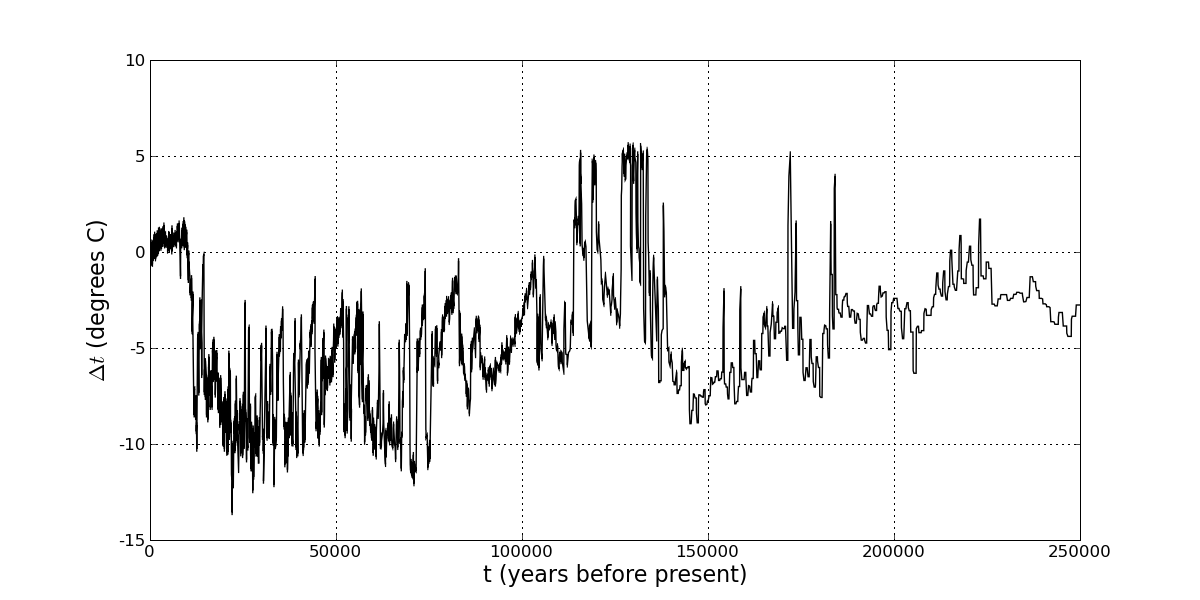
\includegraphics[width=5.6in,keepaspectratio=true]{gripDeltaT}
\caption{Change in temperature from present, from the GRIP core \cite{JohnsenetalGRIP}.}
\label{fig:gripDeltaT}
\end{figure}


\subsubsection*{Bootstrapping}  \label{sect:green-bootstrapping}  Once the EISMINT Greenland data is obtained and converted to NetCDF, as above, ``bootstrapping'' can begin.  By ``bootstrapping'' we mean the creation, by heuristics and simplified models, of the full initial conditions needed for the continuum model.  \footnote{The continuum model is the differential equations describing ice flow inside PISM.  See section \ref{sect:boot} for more on ``bootstrapping''.}

We do a one model year run using option \texttt{-boot_from} to ``bootstrap'' from file \texttt{eis_green_smoothed.nc}.  The executable ``\texttt{pgrn}'' is special to EISMINT-Greenland\footnote{It sets EISMINT-Greenland parameters and implements the elevation- and latitude-dependent near-surface air temperature parameterization but shares all the ice-dynamics code with \texttt{pismr}.}: \index{executables!\texttt{pgrn}}
% pgrn -boot_from eis_green_smoothed.nc -Mx 83 -My 141 -Lz 4000 -Mz 51 -Lbz 2000 -Mbz 21 -skip 1 -y 1 -o green20km_y1.nc
\begin{verbatim}
$ pgrn -boot_from eis_green_smoothed.nc -Mx 83 -My 141 -Lz 4000 -Mz 51 -Lbz 2000 -Mbz 21\
       -skip 1 -y 1 -o green20km_y1.nc
\end{verbatim}%$
\noindent The run takes only a few seconds of real time on any machine.  Tables \ref{bootstrapEISgreen} and \ref{bootCONTINUED} show the entire PISM output at the terminal.

\begin{table}
\centering
\scriptsize
\begin{quote}
\begin{verbatim}
PGRN revision 998:1212M trunk (PISM EISMINT-Greenland mode)
  setting flags equivalent to '-e 3 -ocean_kill'; user options may override ...
Setting PDD parameters to EISMINT-Greenland values...
  pdd_factor_ice  = 0.00879 m (ice equivalent) K-1 day-1
  pdd_factor_snow = 0.00330 m (ice equivalent) K-1 day-1
  pdd_refreeze    = 0.60000 1
  pdd_std_dev     = 5.00000 K
  time dimension was not found; setting current year to 0.0 years
  setting flow law to polythermal type ...
* Initializing Greenland atmosphere model based on the EISMINT Greenland (C. Ritz, 1997)
  air temperature parameterization and using stored time-independent precipitation...
    reading mean annual ice-equivalent snow precipitation rate 'snowprecip'
      from eis_green_smoothed.nc ... 
  FOUND  snowprecip/ mean annual ice-equivalent snow precipitation rate          
                   \ min,max =     0.030,    2.820 (m year-1)
* Initializing the PDD-based surface (snow) processes model...
  Using a PDD implementation based on an expectation integral.
* Initializing the constant ocean model...
bootstrapping by PISM default method from file eis_green_smoothed.nc
  rescaling computational box for ice from -boot_from file and
    user options to dimensions:
    [-820.00 km, 820.00 km] x [-1400.00 km, 1400.00 km] x [0 m, 4000.00 m]
  WARNING: surface elevation 'usurf' found; IGNORING IT!
  reading 2D model state variables by regridding ...
  FOUND  lon       / standard_name=longitude                                                   
                   \ min,max =   -94.194,   12.889 (degree_east)
  FOUND  lat       / standard_name=latitude                                                    
                   \ min,max =    58.275,   84.458 (degree_north)
  FOUND  thk       / standard_name=land_ice_thickness                                          
                   \ min,max =     0.000, 3200.000 (m)
  FOUND  topg      / standard_name=bedrock_altitude                                            
                   \ min,max = -3859.000, 2151.000 (m)
  absent bwat      / effective thickness of subglacial melt water                
                   \ not found; using default constant    0.00 (m)
  absent bmelt     / ice basal melt rate in ice thickness per time               
                   \ not found; using default constant    0.00 (m year-1)
  absent tillphi   / friction angle for till under grounded ice sheet            
                   \ not found; using default constant   15.00 (degrees)
  absent bheatflx  / upward geothermal flux at bedrock surface                   
                   \ not found; using default constant   50.00 (mW m-2)
  absent dbdt      / bedrock uplift rate                                         
                   \ not found; using default constant    0.00 (m year-1)
  determining surface elevation by  usurf = topg + thk           (grounded ice)
        and by flotation criterion  usurf = (1-rho_i/rho_w) thk  (floating ice)
  preliminary determination of mask for grounded/floating and sheet/dragging
    option -ocean_kill seen: floating ice mask=3; ice free ocean mask=7
  filling in ice and bedrock temperatures using surface temps and quartic guess
  ice enthalpy set from temperature, as cold ice (zero liquid fraction)
done reading eis_green_smoothed.nc; bootstrapping done
\end{verbatim}
\end{quote}
\normalsize
\bigskip
\caption{Output of bootstrapping command.  Continues in Table \ref{bootCONTINUED}.}
\label{bootstrapEISgreen}
\end{table}

\begin{table}
\centering
\scriptsize
\begin{quote}
\begin{verbatim}
computational domain and grid:
           spatial domain   1640.00 km x 2800.00 km x (4000.00 m + 2000.00 m bedrock)
            time interval   [ 0.00 a, 1.00 a ]; run length = 1.0000 a
     horizontal grid cell   20.00 km x 20.00 km
  vertical spacing in ice   uneven, 51 levels, 21.200 m < dz < 138.800 m
  vert spacing in bedrock   uneven, 21 levels, 16.875 m < dz < 183.125 m
  initializing bed smoother object with chosen lambda = 5000.000 km half-width
    for intended square smoothing domain ...
    (bed smoother object reports effective lambdax = 20000.000 km, lambday = 20000.000 km)
* Computing corrected cell areas using WGS84 datum...
doing preliminary step to fill diagnostic quantities ...
running forward ...
P         YEAR:     ivol   iarea     thick0     temp0
U        years 10^6_km^3 10^6_km^2        m         K
S      0.00000:  2.82500  1.6708   3042.000  271.0047
 $ SIA v$th d (dt=0.15390)
S      0.15390:  2.82512  2.1980   3041.914  271.0047
 $ SIA v$th d (dt=0.21156)
S      0.36546:  2.82486  1.6728   3041.758  271.0047
 $ SIA v$th d (dt=0.24794)
S      0.61340:  2.82493  1.7320   3041.554  271.0050
 $ SIA v$th d (dt=0.27587)
S      0.88927:  2.82516  2.2300   3041.304  271.0050
 $ SIA v$th e (dt=0.11073)
S      1.00000:  2.82525  2.2300   3041.205  271.0052
done with run ... 
Writing model state to file `green20km_y1.nc'
\end{verbatim}
\end{quote}
\normalsize
\bigskip

\caption{Continuation of Table \ref{bootstrapEISgreen}.}
\label{bootCONTINUED}
\end{table}

What has happened?  As noted, \emph{all} real ice sheet data fails to contain certain variables necessary to initialize an ice sheet model, in the sense of complete initial values for time-dependent partial differential equations.  For instance, the data and the observation-based parameterizations do not include the temperature of the ice anywhere but at the surface.  The data do not include the amount of water stored at the ice/bedrock interface.  And so on.  These are not omissions from the data sets but rather inevitable facts; one cannot observe ice sheets as fluids very well.  Necessarily, therefore, PISM fills in the unknown initial conditions based on some default guesses, as indicated by the messages in Table \ref{bootstrapEISgreen}.

Note that EISMINT-Greenland specifies an 83 by 141 point grid, but you may use other numbers for \texttt{-Mx} and \texttt{-My} if desired.  In such cases the data will be linearly interpolated onto your grid.  Larger values will produce slower runs.

The option \texttt{-boot_from} stands for ``bootstrap from''.  A different option \texttt{-i}, for ``input file'', is used for a file which has full initial conditions.  In practice, \texttt{-i} is only used with a NetCDF file which was previously saved by PISM.  That is, \texttt{-i} is used to continue a run from a saved state.

Note the choice of the height of the computational box (``\texttt{-Lz 4000}''), of the number of vertical levels (``\texttt{-Mz 51}'' for levels in ice and ``\texttt{-Mbz 51}'' for levels in bedrock). The messages to standard out show that the vertical spacing is about 20 m near the base and more than 130 m at the top of the computational box (where it matters less).

We see the report that bootstrapping has applied an interpolation scheme to the surface temperatures and geothermal fluxes to estimate preliminary temperatures within the ice.  It is based on a heuristic for the amount of downward flow in a column.  Thus bootstrapping quickly creates a temperature field at depth, but it is not a field in equilibrium with the flow.  (That's coming \dots)

The bootstrapping mode also fills in several default values.  For instance, the variables \texttt{bwat} (effective thickness of basal water), \texttt{tillphi} (till friction angle), \texttt{bheatflx} (geothermal flux), and \texttt{dbdt} (bed uplift rate) were not found in the input file.   (They would be present in a saved PISM model state and they are part of the ``full initial conditions'' referred to earlier.)  Also, note that the data had redundant surface elevation values in the sense that PISM bootstrapping includes the computation ``\texttt{usurf = topg + thk}'' of the surface elevation from the ice thickness and the bed elevation.

In addition to the default bootstrapping actions there are additional settings special to EISMINT-Greenland.  For instance, because there is no EISMINT-Greenland gridded data set for surface temperature \cite{RitzEISMINT}.  Instead there is a formula (parameterization) which determines the temperature as a function of latitude and surface elevation.  The code behind \texttt{pgrn} knows this formula and uses it.  Also the prescribed constant value for geothermal flux is set.  Finally, by default the option \texttt{-ocean_kill} is set internally in \texttt{pgrn}.  This forces all floating ice to immediately calve off (i.e.~to have thickness zero).

As suggested a few paragraphs back, it is helpful to do a better job of filling in the temperatures within the ice.  One way to do this is to have the temperature field and velocity field co-evolve according to the thermomechanical flow model while holding the upper ice surface stationary.  This is a continuation of ``bootstrapping''.  The effect is to create a temperature field which is approximately stationary with respect to advection and conduction.\footnote{The resulting temperature field is not a fully physical temperature field, however, because it comes from a steadiness assumption about the geometry of the ice sheet.  Said another way, it is a temperature field in equilibrium with a velocity field for which the surface kinematical equation \cite{Fowler} is \emph{not} satisfied.}  We create this temperature field by running for 25000 years\footnote{In fact a longer run is reasonable.  The exponential time constant for decay of the thermomechanically-coupled system toward equilibrium is on the order of 100k years.  But the goal is merely to get to a state which is reasonable for starting a complete steady-state run.} with non-evolving surface.  The option \texttt{-no_mass} turns off the map-plane mass continuity scheme, and thus any evolution of the surface.

\begin{verbatim}
$ mpiexec -n 2 pgrn -i green20km_y1.nc -no_mass -y 25000 -o green20km_Tsteady.nc
\end{verbatim}%$
\noindent This last run takes less than half of a processor-hour.  Parallel processing is effective here, up to perhaps a peak real time speed with 40 processors for this coarse 83$\times$141 grid.  (Finer grid computations, for instance on a 5km grid for a Greenland-sized ice sheet, are \emph{easier} to parallelize in the sense that greater a maximum speedup over one processor is attainable \cite{BBssasliding}.)

The EISMINT-Greenland experiments \cite{RitzEISMINT} specify a positive degree day (PDD) model which is automatically turned on when using the \texttt{pgrn} executable.  (The base executable \texttt{pismr} requires option \texttt{-surface pdd} to turn on the PDD model.)  The PDD model is, by default, implemented by the deterministic scheme described in \cite{CalovGreve05}, but the user can add option \texttt{-pdd_rand} to use a stochastic PDD implementation.  The temperature parameterization and positive degree day factors are from \cite{RitzEISMINT} instead of the default for \texttt{pismr}, which uses \cite{Faustoetal2009}.


\subsubsection*{Running the EISMINT-Greenland steady state experiments}  Now that we have initial conditions including a vaguely-credible temperature field, our first experiment is the steady state run ``SSL2'' (turned on using the option \intextoption{ssl2}).  This experiment uses the parameters specified in the EISMINT-Greenland description \cite{RitzEISMINT}.  If 8 processors are used, a ten thousand model year run might look like this:

\begin{verbatim}
$ mpiexec -n 8 pgrn -ssl2 -i green20km_Tsteady.nc -y 10000 -ys 0 \
          -o green_SSL2_10k.nc
\end{verbatim}%$
\noindent We could continue for another ten thousand years by starting from the saved file and continuing for 10000 more model years:
\begin{verbatim}
$ mpiexec -n 8 pgrn -ssl2 -i green_SSL2_10k.nc -y 10000 \
          -o green_SSL2_20k.nc
\end{verbatim}%$
\noindent And so on.

The script \texttt{ssh2.sh} uses options \texttt{ts_file} and \texttt{save_file} to do the run with ``snapshots'' saved every 10000 model years, and the volume saved every 100 model years.  So out discussion will now assume that the user \emph{actually} did this to completion:

\begin{verbatim}
./ssh2.sh 2 >> out.ssl2 &
\end{verbatim}

\noindent This puts the run in the background and generates a text file logging the whole run.  The whole SSL2 run should take something like ?? processor hours.  Three files appear, \texttt{vol_ssl2.nc}, \texttt{snaps_ssl2.nc}, and, at the end of the run, \texttt{green_ssl2_110ka.nc}.

The SSL2 simulation is intended to go until the model reaches a ``steady state'', a phrase which \cite{RitzEISMINT} defines as a small volume change rate, namely less than a .01\% change in volume in 10,000 years.  One can look at the standard output text file by a minimal method like ``\texttt{less out.ssl2}''.  The user can more clearly see the behavior over time of the volume, area, basal melt fraction, and a couple of other default quantities, by viewing the NetCDF file \texttt{vol_ssl2.nc}.  We leave it as an exercise to find the first 10000 model year period in which the volume changes by less that 0.01\%.

In any case, one sees that the volume shows a consistent growing-but-leveling-out trend, with a final volume a bit more than $4 \times 10^{6}\,\text{km}^3$.  The time series for volume and melt fraction (the fraction of the base where the temperature is at pressure-melting) are shown in Figures \ref{fig:eisgrnvolseries} and \ref{fig:eisgrnmeltfseries}.  The volume time series is boring, but the melt fraction indicates something interesting: measured by basal melt fraction, the temperature field resulting from bootstrapping and relaxing the temperature field (above) gave a pretty good estimate of the basal melt fraction for the fully coupled steady state.

\begin{figure}[ht]
\centering
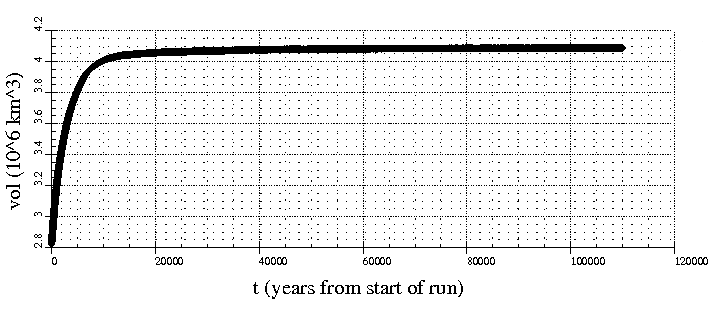
\includegraphics[width=6.0in,keepaspectratio=true]{eisgrn-volseries}
\caption{Volume time series for a 110k model year EISMINT-Greenland SSL2 run; units of $10^{6}\,\text{km}^3$.}
\label{fig:eisgrnvolseries}
\end{figure}

\begin{figure}[ht]
\centering
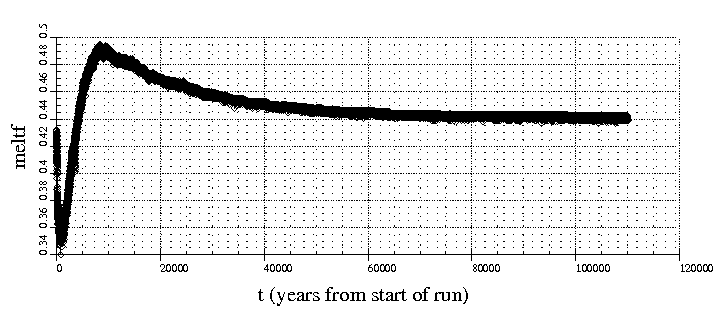
\includegraphics[width=6.0in,keepaspectratio=true]{eisgrn-meltfseries}
\caption{Time series for the fraction of the base which is at the pressure-melting temperature from a 110k model year EISMINT-Greenland run.  See the right hand part of Figure \ref{fig:ssl2thickTpa} for a map of the basal temperature.}
\label{fig:eisgrnmeltfseries}
\end{figure}

We will use the final NetCDF file \texttt{green_ssl2_110ka.nc} to continue the EISMINT-Greenland experiments below.  The saved ice thickness, basal temperature, and vertically-averaged horizontal velocity maps are shown in Figure \ref{fig:ssl2thickTpa}.

\begin{figure}[ht]
\centering
\mbox{\phantom{|}\hspace{-1.0in}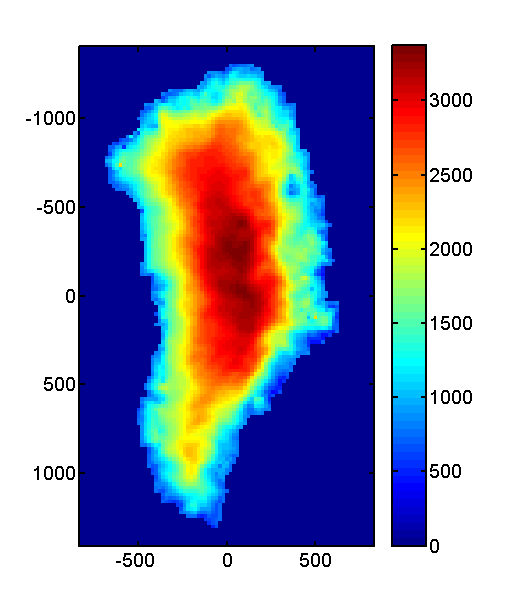
\includegraphics[height=3.0in,keepaspectratio=true]{greenH-SSL2}\,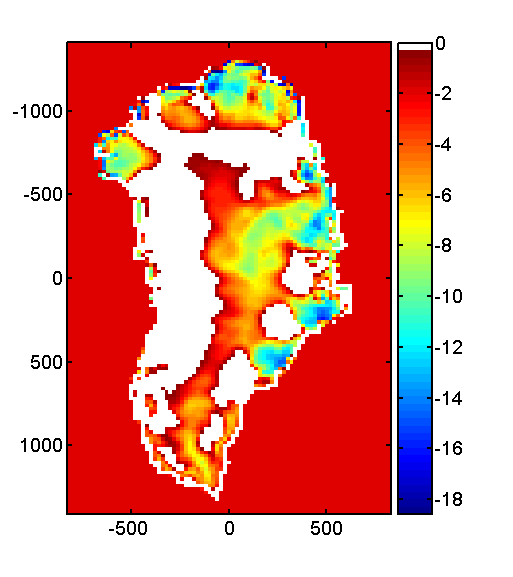
\includegraphics[height=3.0in,width=2.3in]{greenTpa-SSL2}\,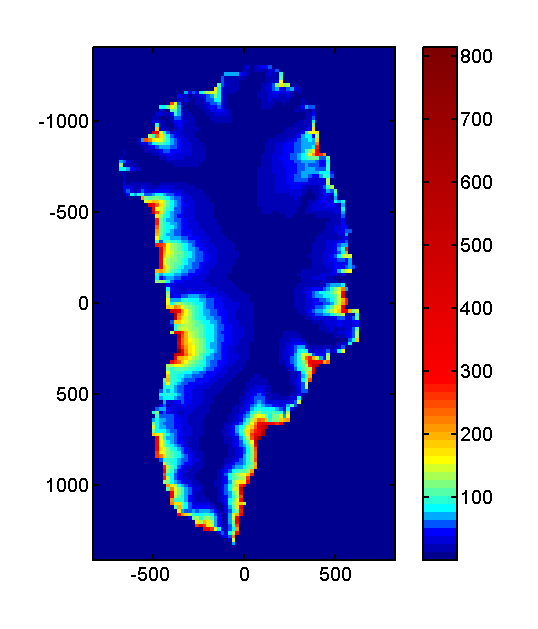
\includegraphics[height=3.0in,keepaspectratio=true]{greencbar-SSL2}}
%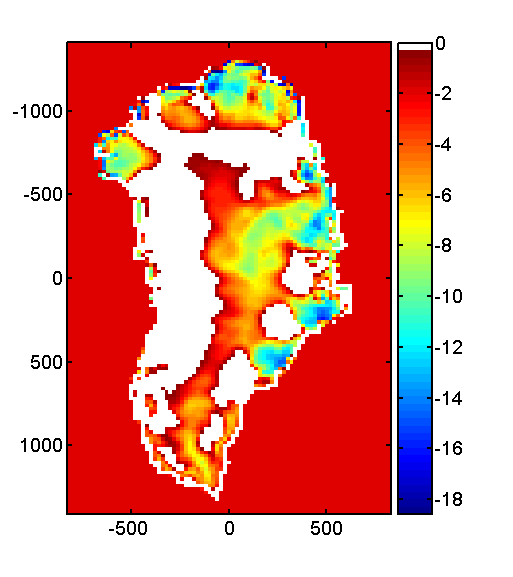
\includegraphics[height=3.7in,width=2.9in]{greenTpa-SSL2}
\caption{Ice thickness (meters; left), basal temperature (degrees C below 0; middle), and vertically-averaged horizontal velocity (m/a; right) at the end (110k model years) of a EISMINT-Greenland SSL2 run.  Note that in the temperature graph the pressure-melting temperature areas are white.}
\label{fig:ssl2thickTpa}
\end{figure}

In addition to the more standardized EISMINT-Greenland intercomparison called ``SSL2'', a ``SSL3'' was proposed to allow each participant to choose additional parameters and adjust other aspects of the model.  (Sliding, for instance, is an outstanding omission here.)  We omit this run for tutorial purposes, however, and proceed to use climate forcing in runs ``CCL3'' and ``GWL3''.


\subsubsection*{Climate forcing from GRIP and SPECMAP} 
\label{sec:climate-forcing}
The next experiment starts from the end of the steady state SSL2 run above.  Recall that the NetCDF files \texttt{grip_dT.nc} and \texttt{specmap_dSL.nc} contain time series data for change in surface temperature and sea level.  The options \texttt{-dTforcing} and \texttt{-dSLforcing} include these data for a ``CCL3'' climate forced run \cite{RitzEISMINT,HuybrechtsEISMINT}.  Before every time step, \texttt{pgrn} reads the change to the surface temperature and sea level for that time.  The data in \texttt{grip_dT.nc} extends 250,000 years into the past, while the data in \texttt{specmap_dSL.nc} goes back about 780,000 years, so EISMINT-Greenland specifies that the run will start at the beginning of the GRIP data.  

The script \texttt{ccl3.sh} runs the CCL3 experiment for the full 250ka period, with this single command
\begin{verbatim}
mpiexec -n 8 pgrn -ccl3 -skip 10 -i green_ssl2_110ka.nc -ys -249900 -ye 0 \
        -atmosphere eismint_greenland,forcing -ocean constant,forcing \
        -dTforcing grip_dT.nc -dSLforcing specmap_dSL.nc \
        -save_file snaps_ccl3.nc -save_times -240000:10000:-10000 \
        -ts_file vol_ccl3.nc -ts_vars ivol -ts_times -249900:100:0 \
        -o green_ccl3_year0.nc
\end{verbatim}
\noindent Option \intextoption{ccl3} also turns on the Lingle and Clark \cite{BLKfastearth,LingleClark} two layer, flat earth bed deformation model with an assumption of zero uplift rate at the start of the run.

The resulting thickness difference, relative to the end of the SSL2 run, and the pressure-adjusted basal temperature, are shown in Figure \ref{fig:cclthickTpa}.

\begin{figure}[ht]
\centering
\includegraphics[width=2.8in]{Hdiff-CCLSSL}\quad\includegraphics[width=2.8in]{Tpa-CCL}
\caption{Left:  Ice thickness difference between end (year zero) of a CCL3 run and the end of an SSL2 run (meters).  Right:  Ice pressure-adjusted basal temperature (degrees C below 0; right) at the end of a EISMINT-Greenland CCL3 run.  Compare Figure \ref{fig:ssl2thickTpa}.}
\label{fig:cclthickTpa}
\end{figure}

EISMINT-Greenland also calls for a baseline run for another 500 years which starts from the end of the CCL3 run and has steady current climate forcing (noting no GRIP or SPECMAP data are known from the future!):

\begin{verbatim}
mpiexec -n 8 pgrn -ccl3 -i green_ccl3_year0.nc -y 500 -o green_ccl3_year500.nc
\end{verbatim}

A final ``greenhouse warming'' experiment ``GWL3'' (options \intextoption{gwl3} and \intextoption{gwl3_start_year}) is described in the EISMINT-Greenland \cite{RitzEISMINT}.  It runs for 500 years with the temperature increasing by $0.035^\circ C/$year for the first 80 years, then at a rate of $0.0017^\circ C/$year for the last 420 years:

\begin{verbatim}
mpiexec -n 8 pgrn -gwl3 -i green_ccl3_year0.nc -y 500 -o green_gwl3_year500.nc
\end{verbatim}

\subsubsection*{Visualizing the climate inputs in the Greenland case}
\label{sec:pdd-series-with-pclimate}

Assuming that \texttt{green20km_y1.nc} was produced by the run above (see section
\ref{sect:green-bootstrapping}), one can run the following to check if the PDD
model in PISM (see section \ref{sec:boundary-models}) is ``reasonable'':
% pclimate -i green20km_y1.nc -atmosphere eismint_greenland -surface pdd -ys 0.0 -ye 2.5 -dt 0.1 -o pddmovie.nc 
\begin{verbatim}
$ pclimate -i green20km_y1.nc -atmosphere eismint_greenland -surface pdd \
           -ys 0.0 -ye 2.5 -dt 0.1 -o pddmovie.nc 
\end{verbatim}%$
This produces the file \texttt{pddmovie.nc} with several variables: \texttt{acab}
(instantaneous net ice equivalent accumulation (ablation) rate), \texttt{artm}
(mean annual temperature at ice surface but below firn), \texttt{snowtemp}
(instantaneous snow temperature), \texttt{snowprecip} (mean annual
ice-equivalent snow accumulation rate) and some others.

Variables \texttt{artm} and \texttt{snowprecip} do not evolve over time because the 
former is generated from ice sheet geometry and latitude by the EISMINT-Greenland
formulas \cite{RitzEISMINT}, while the latter is part of the EISMINT-Greenland data
itself.

The other two variables were used to create figure \ref{fig:pddseries}, which
shows the time-series of the accumulation rate (top graph) and the snow
temperature (bottom graph) with the map view of the snow temperature at time 0
over it. The cross on the latter shows (approximately) the location of the
point used for the time-series.

Here are two things to notice:
\begin{enumerate}
\item The summer peak day is in the right place.  The default for this value is
  August 1 (day $243$, at approximately $243/365 \simeq 0.66$ year).  (If it is
  important, the peak day can be changed using the \texttt{-pdd_summer_peak_day}
  option; subsection \ref{sec:boundary-models}).

\item Lows of the surface mass balance rate \texttt{acab} correspond to 
  positive degree-days in the given period, because of highs of the snow 
  temperature.  Recall the snow temperature graph does
  not show random daily variations.  Even though it has the maximum of about $266$
  Kelvin, the parameterized instantaneous snow temperature can be above freezing.
  A positive value for positive degree-days is expected \cite{CalovGreve05}.
\end{enumerate}

\begin{figure}[ht]
  \centering
  \includegraphics[width=5in]{pdd-timeseries}
  \caption{Time series of the surface mass balance rate and snow temperature. Map view 
           on the right shows the location chosen.}
  \label{fig:pddseries}
\end{figure}

\bigskip
We can also test the surface temperature forcing code with the following command.
% pclimate -i green20km_y1.nc -o dT_movie.nc -atmosphere eismint_greenland,forcing -dTforcing grip_dT.nc -ys -2.5e5 -ye 0 -dt 2000
\begin{verbatim}
$ pclimate -i green20km_y1.nc -o dT_movie.nc \
           -atmosphere eismint_greenland,forcing -dTforcing grip_dT.nc \
           -ys -2.5e5 -ye 0 -dt 2000
\end{verbatim}%$
The output \texttt{dT_movie.nc} and \texttt{grip_dT.nc} mentioned in section above were used to create figure \ref{fig:artm-timeseries}.

This figure shows the GRIP temperature offsets (top graph; compare to figure \ref{fig:gripDeltaT}) and the time-series of the temperature at the ice surface at a point in southern Greenland (bottom graph), confirming that the temperature offsets are used correctly.

\begin{figure}[ht]
  \centering
  \includegraphics[width=5in]{artm-timeseries}
  \caption{Time series of the surface temperature compared to GRIP temperature offsets}
  \label{fig:artm-timeseries}
\end{figure}

\begin{comment}
  FIXME: Variable acab in following is worth looking at. It looks right and it
  may be possible to compare to other paleo-limate studies:
% pclimate -i green20km_y1.nc -o bar.nc -ys -125000.0 -ye -0.0 -dt 1000.0  -dTforcing grip_dT.nc -dSLforcing specmap_dSL.nc -atmosphere eismint_greenland,forcing -surface pdd -ocean constant,forcing
\begin{verbatim}
$ pclimate -i green20km_y1.nc -o bar.nc -ys -125000.0 -ye -0.0 -dt 1000.0 \
           -dTforcing grip_dT.nc -dSLforcing specmap_dSL.nc \
           -atmosphere eismint_greenland,forcing -surface pdd -ocean constant,forcing
\end{verbatim}%$
\end{comment}

%%% Local Variables: 
%%% mode: latex
%%% TeX-master: "manual"
%%% End: 

% LocalWords:  parameterized


\clearpage\newpage

\section{Example: Validating PISM as a flow model for the Ross ice shelf (EISMINT-Ross)}\label{sect:ross} \index{PISM!running the EISMINT-Ross ice shelf intercomparison in}\index{Ice Sheets!Antarctic ice sheet!Ross ice shelf} \index{EISMINT!intercomparison of Ross ice shelf models} \index{PISM!validation of ice shelf model} \index{Ross ice shelf}
\optsection{EISMINT-Ross}

The term ``validation'' describes the comparison of model output with physical observations in cases where those physical observations are believed to be sufficiently complete and of sufficient quality so that the performance of the numerical model can be assessed \cite{Roache,Wesseling}.  Roughly speaking, validation can happen when the observations or data are better than the model, so the comparison measures the quality of the numerical model and not merely errors in, incompleteness of, or lack of confidence in, the data.

As part of the first EISMINT series of intercomparisons, MacAyeal and others \cite{MacAyealetal} validated several ice shelf numerical models using the Ross ice shelf as an example.  We refer to this intercomparison and its associate write-up \cite{MacAyealetal} as ``EISMINT-Ross''.  The models were compared to data from RIGGS (the Ross Ice shelf Geophysical and Glaciological Survey \cite{RIGGS2,RIGGS1}), acquired in the period 1973--1978.   The RIGGS data include the (horizontal) velocity of the ice shelf measured at a few hundred locations in a reasonably regular grid across the shelf; see figure \ref{fig:rosspython} below for an indication of these positions.

Substantial developments have occurred in the modeling of the Ross ice shelf since the EISMINT-Ross intercomparison.  For example, inverse modeling techniques were used to recover depth-averaged viscosity of the Ross ice shelf from the RIGGS data in \cite{RommelaereMacAyeal}. A parameter-sensitivity study was performed for a particular Ross ice shelf numerical model in \cite{HumbertGreveHutter}.

The scripts in this section are found in the directory \texttt{examples/eisross/}.  The script \texttt{quickstart.sh} in that directory will download the data, build a NetCDF input file, and run \texttt{pross} as described in the next three subsections.

\subsubsection*{Grabbing the data}  Download data files from the website:

\centerline{\url{http://homepages.vub.ac.be/~phuybrec/eismint/iceshelf.html}}
\small

\begin{verbatim}
$ cd examples/eisross/
$ wget http://homepages.vub.ac.be/~phuybrec/eismint/111by147Grid.dat
$ wget http://homepages.vub.ac.be/~phuybrec/eismint/kbc.dat
$ wget http://homepages.vub.ac.be/~phuybrec/eismint/inlets.dat
\end{verbatim}
\normalsize The reader might want to look at these files in a text editor.  Their idiosyncratic format must be handled by a python script, namely \texttt{eisross.py} below.  In fact, a significant part of setting up EISMINT-Ross in PISM was the step of converting these text files into a machine-readable and metadata-containing NetCDF file.  The next script\footnote{Requires \href{http://numpy.scipy.org/}{\texttt{numpy}} and \href{http://code.google.com/p/netcdf4-python/}{\texttt{netcdf4-python}}.} reads the above three \texttt{.dat} files and it creates a NetCDF file:

\begin{verbatim}
$ ./eisross.py -o ross.nc
\end{verbatim}
Note that the NetCDF file \texttt{ross.nc} can be reconverted to text (CDL) using \texttt{ncdump} or it can be viewed graphically with \texttt{ncview}.  For example, \texttt{ncdump -h ross.nc} shows the ``header'' (the metadata) for \texttt{ross.nc}.  The script \texttt{eisross.py} has added this metadata, much of which can only be found by carefully reading references \cite{RIGGS2,RIGGS1,MacAyealetal}.

\begin{figure}[ht]
\centering
\includegraphics[height=2.3in,keepaspectratio=true]{rossmask} \qquad \includegraphics[height=2.3in,keepaspectratio=true]{rossubar}
\caption{Two views from \protect{\texttt{ncview}} of the EISMINT-Ross data in the NetCDF file \protect{\texttt{ross.nc}}.  The floating-versus-grounded mask (left; red areas are floating ice shelf) and the $x$-component of the non-zero kinematic (Dirichlet) boundary condition for velocity (right).}
\label{fig:rossmaskubar}
\end{figure}

The NetCDF file \texttt{ross.nc} contains ice thickness, bed elevations, surface temperature, and accumulation.  Values for latitude and longitude from the RIGGS survey grid \cite{RIGGS1} are given.  All of these are typical of ice sheet modeling data, both in evolution and diagnostic runs.  The file also has variables \texttt{ubar} and \texttt{vbar}.  These give the boundary values which are needed for the diagnostic computation of velocity, and they are only valid at grounding line locations.  They are the measured velocities of the ice flow inputs to the ice shelf.  Also present are integer variables \texttt{mask}, which shows the domain where the ice shelf is modeled, and \texttt{bcflag}, which shows the locations where the boundary conditions are to be applied.  Finally, \texttt{ross.nc} contains variables which allow us to partly validate our computation.  There is an interger variable \texttt{accur} which flags the region where the interpolated measured velocities are believed to be accurate enough for validation.\footnote{\texttt{111by147.dat} has a ``Reliable Velocity Obs'' flag.}  The variables \texttt{azi_obs} and \texttt{mag_obs} are believed to be accurate in this region \cite{MacAyealetal}.

The original EISMINT-Ross data are on a 111 by 147 grid but \texttt{eisross.py} extends this grid to a more convenient 147 by 147 grid with the same $6.822$ km spacing.  This grid has ice-free ocean beyond the calving front, which is straightened as described in \cite{MacAyealetal}.  The gridded data have a particular resolution, but the PISM computational grid can be finer or coarser according to runtime options (as illustrated below).

\subsubsection*{Diagnostic computation of ice shelf velocity}  A basic Ross ice shelf velocity computation from these data is:

\begin{verbatim}
$pross -boot_file ross.nc -ssaBC ross.nc -Mx 147 -My 147 -Mz 3 -Lz 1e3
\end{verbatim}
Here we bootstrap (\texttt{-boot_file}; see section \ref{sect:boot}) from \texttt{ross.nc}.  We also use a special option \texttt{-ssaBC} to specify \texttt{ross.nc} as the source of the boundary value data for the ice shelf equations, as mentioned in the last paragraph.  The computational grid specified here is the $6.822$ km data grid in EISMINT-Ross with 147 grid points in each direction.  The maximum thickness of the ice is 874 m so we choose a height for the computational box (\texttt{-Lz}) large enough to contain the ice.  Note that using a small number of vertical levels (\texttt{-Mz 11}) is reasonable because the EISMINT-Ross intercomparison specifies that the temperature at each depth is just the surface temperature \cite{MacAyealetal}.  In fact there is no thermocoupling issue because the ice hardness used here is constant.

At the end of this run the computed velocity field is compared to the interpolated observed velocities stored in \texttt{ross.nc}.  The value called ``average relative error in vector vel'' is most relevant.  A value of 0.07 here means that the averaged absolute difference between the computed and the observed velocity, in the ``accurate'' region, is 7\%.

The output file \texttt{unnamed_diag.nc} contains vertically-averaged horizontal speed in the variable \texttt{cbar}.  Figure \ref{fig:rosspython} shows that computed speed as the color background; the comparison of modeled and observed vector velocities in that figure is discussed below.

There are many variations on this basic ``\texttt{pross}'' run above.  First of all one can get more information during the run by adding diagnostic viewers and a more complete (verbose) report to standard out:
% pross -boot_file ross.nc -ssaBC ross.nc -Mx 147 -My 147 -Mz 3 -Lz 1e3 -view_map cbar,mask,log_nuH,uvbar -verbose -pause 10
\begin{verbatim}
$ pross -boot_file ross.nc -ssaBC ross.nc -Mx 147 -My 147 -Mz 3 -Lz 1e3 \
        -view_map cbar,mask,log_nuH,ubar -verbose -pause 10
\end{verbatim}
Secondly one might want to do the run in parallel and do it on a finer grid.  For example,

\begin{verbatim}
$ mpiexec -n 4 pross -boot_file ross.nc -ssaBC ross.nc \
          -Mx 201 -My 201 -Mz 3 -Lz 1e3
\end{verbatim}
The result is very similar, as it should be.  On the other hand, since the data is only on a 6.8 km grid we expect no added accuracy on this new 5km grid.

Alternately one might want to experiment with different values of the hardness parameter.  Its default value is $\bar B = 1.9 \times 10^8 \, \text{Pa}\, \text{s}^{1/3}$ as in \cite{MacAyealetal}.   We can also use smaller (more severe) tolerances for the nonlinear iteration (\intextoption{ssa_rtol}) and the linear iteration (\intextoption{ksp_rtol}) to get more confidence in the numerical scheme:

\begin{verbatim}
$ pross -boot_file ross.nc -ssaBC ross.nc -Mx 147 -My 147 -Lz 1000 \
        -Mz 11 -ssa -ice_type custom -ice_custom_hardness 1.8e8 \
        -o ross_out_1p8.nc -ssa_rtol 1e-6 -ksp_rtol 1e-10
\end{verbatim}


\subsubsection*{Comparison to RIGGS data}  The file \texttt{riggs_clean.dat} is a cleaned-up version of the original RIGGS\index{RIGGS} data \cite{RIGGS1, RIGGS2}.  (See \texttt{README} for more explanation on this RIGGS data.)  To convert this data to a NetCDF file, as needed next, do

\begin{verbatim}
./riggs.py -o riggs.nc
\end{verbatim}
A file \texttt{riggs.nc} will be created.  This data is one-dimensional; it is just a lists of values which have an index dimension \texttt{count} in the NetCDF file \texttt{riggs.nc}.

Now, \texttt{pross} can read this data and compute a $\chi^2$ statistic comparing computed PISM output to the data:

\small
\begin{verbatim}
$ pross -boot_file ross.nc -Mx 147 -My 147 -Lz 1e3 -Mz 3 \
        -ssaBC ross.nc -riggs riggs.nc
PROSS revision 1073M trunk (EISMINT-Ross diagnostic velocity computation mode)
. . .
initializing EISMINT-Ross ice shelf velocity computation ... 
. . .
maximum computed speed in ice shelf is   1365.053 (m/a)
. . .
comparing to RIGGS data in riggs.nc ...
. . .
Chi^2 statistic for computed results compared to RIGGS is   3638.850
Writing model state to file `rossComputed.nc'
\end{verbatim}
\normalsize

Naturally, the question is ``does this $\chi^2$ value of $3639$ represent a good fit of model result to observations''?  Also naturally, there is no objective answer.  For comparison, Table 1 in \cite{MacAyealetal} is reproduced here as Table \ref{tab:chisqr}.  As noted, all these results are with a constant hardness parameter $\bar B = 1.9 \times 10^8 \, \text{Pa}\, \text{s}^{1/3}$ \cite{MacAyealetal}. The maximum computed horizontal ice speed above of $1365$ m/a is slightly lower than the maximum velocities reported by the other models but, on the other hand, the maximum measured speed in the RIGGS data set is $1007$ m/a (occurring near the calving front, naturally).  The $\chi^2$ result is essentially as good as the best in the Table, noting smaller $\chi^2$ is better.

\small
\begin{table}[ht]
\centering
\caption{Model performance index, $\chi^2$ (non-dimensional).  \protect{\textsl{(Reproduction of Table 1 in \cite{MacAyealetal}.)}}}\label{tab:chisqr}
\begin{tabular}{p{0.2\linewidth}p{0.1\linewidth}p{0.3\linewidth}}\toprule
\textsl{Model} & $\chi^2$ & \textsl{Maximum velocity, m/year} \\\midrule
Bremerhaven1 & 3605 & 1379 \\
Bremerhaven2 & 12\,518 & 1663 \\
Chicago1 & 5114 & 1497 \\
Chicago2 & 5125 & 1497 \\
Grenoble & 5237 & 1508 \\
\bottomrule
\end{tabular}
\end{table}
\normalsize

\subsubsection*{Tuning the ice hardness for a better fit to RIGGS}  Because there is a relatively rich data set from RIGGS on ice velocity, it is reasonable to ask whether the PISM computed velocities can fit the data better if the spatially-constant hardness parameter $\bar B$ is adjusted.  In directory \texttt{examples/eisross/} there is a Python script \texttt{tune.py} which (by default) runs \texttt{pross} with seven values of $\bar B$ ranging from $\bar B = 1.6  \times 10^8$ to $\bar B = 2.2 \times 10^8 \, \text{Pa}\, \text{s}^{1/3}$.  It uses smaller values for the convergence tolerances (by default), yielding slightly different $\chi^2$ values.  It can be run in parallel: ``\texttt{\$ ./tune.py -n 4}.''

One sees that hardnesses $\bar B = 1.9,2.0 \times 10^8 \, \text{Pa}\, \text{s}^{1/3}$ give the best fits, by the standard of $\chi^2$ relative to RIGGS data.  This fitting exercise is a first small step towards inverse modelling of the spatially-distributed effective viscosity.  Another major tunable parameter, not demonstrated with \texttt{tune.py}, is the calving front force boundary condition.  More steps in the inverse modeling direction, for modeled velocity in Antarctic ice shelves, are found in \cite{HumbertGreveHutter,RommelaereMacAyeal}.


\subsubsection*{Additional visualization}  The visualization abilities of PISM's runtime viewers, and of \texttt{ncview} for NetCDF files, are limited.  On the other hand, we can produce pretty pictures using Python.  The script \texttt{rossplot.py} uses Python packages \texttt{netcdf4-python}, \texttt{matplotlib}, and \t{scikits.delaunay} to do this.  Assuming that files \texttt{ross.nc} and \texttt{rossComputed.nc} were produced as described previously, and are in the current directory, and that file \texttt{riggs_clean.dat} is present in the current directory too, then we can do:

\begin{verbatim}
$ ./rossplot.py
\end{verbatim}

\noindent We get Figure \ref{fig:rosspython}.  We have succeeded in modeling the flow in a real ice shelf.

\begin{figure}[ht]
\centering
\mbox{\includegraphics[width=3.3in,keepaspectratio=true]{rossquiver}\quad \includegraphics[width=2.7in,keepaspectratio=true]{rossscatter}}
\caption{\protect{\emph{Left}}: Color is speed in m/a.  Arrows are observed (black) and computed (red) velocities at RIGGS points.  \protect{\emph{Right}}: Comparison between modeled and observed speeds at RIGGS points; compare Figure 2 in \cite{MacAyealetal}.}
\label{fig:rosspython}
\end{figure}


%%% Local Variables: 
%%% mode: latex
%%% TeX-master: "manual"
%%% End: 



%         References
\clearpage\newpage
\bibliography{ice-bib}
\bibliographystyle{siam}

\appendix

\newcommand{\subsect}[1]{\bigskip\subsection{#1}\rule{0mm}{2mm}\par\medskip}
%\newcommand{\subsectstar}[1]{\bigskip\subsection*{#1}\rule{0mm}{2mm}\par\medskip}
\newcommand{\subsectstar}[1]{\bigskip\noindent\textbf{#1.}\rule{0mm}{2mm}\par\medskip}
\newcommand{\subsubsect}[1]{\subsubsection{#1}\rule{0mm}{2mm}\par\smallskip}

\clearpage\newpage
\section{PISM command line options}\label{sect:options}

As PISM is a PETSc program \cite{petsc-user-ref}, all PETSc options are available as well.  The last subsection \ref{subsect:petscoptions} recalls some of these PETSc options.

The Index on page \pageref{sect:index} contains an alphabetical list of options.

\optsection{Old option index}
\subsect{List of PISM options}

\subsectstar{Options turning on and off major physical models}

\opt{float_kill}  If ice is (or becomes) floating then it is set to thickness zero.  This is calving at the grounding line.

\opt{hold_tauc}    Keep the current values of the till yield stress $\tau_c$.  That is, do not update them by the default model using the stored basal melt water.  Only effective if \texttt{-ssa} and \texttt{-plastic} are also set.  See documentation of option \texttt{-plastic} for a description of the till yield stress model.

\opt{no_mass}  Forces PISM to not change the ice thickness.  No time steps of the mass conservation equation are computed.

\opt{no_temp}  Force PISM to not change temperature or age values within the ice.  No time steps of the energy conservation and age equations are computed.

\opt{ocean_kill}  If used with input from a NetCDF initialization file which has ice-free ocean mask (value \texttt{MASK_FLOATING_OCEAN0}$=7$), will zero out ice thicknesses in areas that were ice-free ocean at time zero.  This is calving at the location of the original calving front.  Has no effect when used in conjunction with \texttt{-no_mass}.

\opt{ssa}  Use the equations of the shallow shelf approximation \cite{MacAyeal,Morland,SchoofStream,WeisGreveHutter} for ice shelves and dragging ice shelves (i.e.~ice streams) where so-indicated by the mask.  To view the mask use \texttt{-view_map mask}.  See also \texttt{-plastic} and \texttt{-super}. See also \texttt{-dontreadSSAvels}.

\opt{super}  Combine the velocity fields from the SIA and SSA models as in \cite{BBssasliding}.  Only effective if used with \texttt{-ssa}.

\subsectstar{Options controlling numerical methods}

\subsubsect{General methods}

\opt{eta}  The surface gradient is usually computed in the obvious way by finite differences applied to the surface elevation $h$.  Specifically, we use the Mahaffy \cite{Mahaffy} scheme.  Alternatively, if this option is set we first transform the thickness $H$ by $\eta = H^{(2n+2)/n}$ and then differentiating the sum of the thickness and the bed:
	$$\grad h = \grad H + \grad b = \frac{n}{(2n+2)} \eta^{(-n-2)/(2n+2)} \nabla \eta + \nabla b.$$
Here $b$ is the bed elevation and $h$ is the surface elevation.  The transformation sometimes has the benefits that the surface values of the horizontal velocity and vertical velocity, and the driving stress, are better behaved near the margin.  See \cite{CDDSV} for the technical explanation of this transformation and compare \cite{SaitoMargin}.

\optdef{low_temp}{200.0}  Set the temperature which PISM will regard as ``too low''.  Units in Kelvin.  Note that one kind of numerical error associated to the advection part of the conservation of energy scheme is for the maximum principle to be violated.  In that case temperatures appear at the next step which are outside the range of current temperatures.  PISM attempts to count such violations, and if the number is too great then the run is stopped.  See option \texttt{-max_low_temps}.

\optdef{max_low_temps}{10}  Specify the number (a nonnegative integer) of allowed low temp violations per time step.  Note these are reported in detail (i.e.~with location) if \texttt{-verbose} is set.  Note that one kind of numerical error associated to the advection part of the conservation of energy scheme is for the maximum principle to be violated.  In that case temperatures appear at the next step which are outside the range of current temperatures.  PISM attempts to count such violations, and if the number is too great then the run is stopped.  See option \texttt{-low_temp} for the cutoff low temperature.

% FIXME: describe the pross driver.
% \optrestrict{ross}{pismd}    Run the EISMINT Ross ice shelf validation \cite{MacAyealetal}.  Requires data from \url{http://homepages.vub.ac.be/~phuybrec/eismint/iceshelf.html}.


\subsect{PETSC options for PISM users}\label{subsect:petscoptions}

All PETSc programs accept command line options which control how PETSc distributes jobs among parallel processors, how it solves linear systems, what additional information it provides, and so on.  The PETSc manual \cite{petsc-user-ref} is the complete reference on these options.  We list some here that are useful to PISM users.  They can be mixed in any order with PISM options.

Both for PISM and PETSc options, there are ways of avoiding the inconvenience of long commands with many runtime options.  Obviously, and as illustrated by examples in the previous sections, shell scripts can be set up to run PISM.  But PETSc also provides two mechanisms to give runtime options without retyping at each run command.

First, the environment variable \texttt{PETSC_OPTIONS} can be set.  For example, a sequence of runs might need the same refined grid, and you might want to know if other options are read, ignored, or misspelled.  Set (in bash):

\texttt{export PETSC_OPTIONS="-Mx 101 -My 101 -Mz 51 -options_left"}

\noindent The runs 
\begin{verbatim}
$ pismv -test F -y 100
$ pismv -test G -y 100
\end{verbatim}
\noindent then have the same refined grid in each run, and the runs report on which options were read.

Second, the file \texttt{.petscrc} is always read, if present, from the directory where PISM (i.e.~the PETSc program) is started.  It can have a list of options, one per line.  For example, to get the same options as above, \texttt{.petscrc} would contain these lines:
\begin{verbatim}
-Mx 101
-My 101
-Mz 51
-options_left
\end{verbatim}
\noindent Note that the first four lines give PISM options while the last has a generic PETSc option.

These two PETSc mechanisms can be used together.  (The effect of duplicate or conflicting options is not clear, however, and should be avoided.)
\bigskip

% "-da_processors_x M -da_processors_y N" should not be documented in this sub-appendix
% because they do not work.  the reason is that IceModelVec2 and IceModelVec3 put 
% the Mx, My dimensions in different arguments to the DACreate commands


\optdef{ksp_rtol}{1e-5}  For solving the SSA equations with high resolution on multiple processors, it is recommended that this be tightened (set lower than the default).  For example, 

\verb|$  mpiexec -n 8 pismv -test I -Mx 5 -My 769|

\noindent works poorly on a certain machine, but

\verb|$  mpiexec -n 8 pismv -test I -Mx 5 -My 769 -ksp_rtol 1e-10|

\noindent works fine.

\optdef{ksp_type}{gmres}  Based on one processor evidence from \texttt{pismv -test I}, the following are possible choices in the sense that they work and allow convergence at some reasonable rate: \t{cg}, \t{bicg}, \t{gmres}, \t{bcgs}, \t{cgs}, \t{tfqmr}, \t{tcqmr}, and \t{cr}.  It appears \t{bicg}, \t{gmres}, \t{bcgs}, and \t{tfqmr}, at least, are all among the best.



\optdef{pc_type}{ilu}   Several options are possible, but for solving the ice stream and shelf equations we recommend only \t{bjacobi}, \t{ilu}, and \t{asm}.  Of these it is not currently clear which is fastest; they are all about the same for \texttt{pismv -test I} with high tolerances (e.g.~\texttt{-ssa_rtol 1e-7} \texttt{-ksp_rtol 1e-12}).




\phantomsection
\addcontentsline{toc}{section}{General Index}
\label{sect:index}
\printindex

\phantomsection
\addcontentsline{toc}{section}{PISM Command-line options}
\printindex[options]


\end{document}
